% Sample Dissertation, Thesis, or Document %
%            for use with the              %
%  University of Arizona Thesis Class,     %
%               uathesis.cls               %
%------------------------------------------%

% We'll use the uathesis document class (duh).  The uncommented line
% below will produce a Dissertation, the others would produce a Thesis
% or a Document.  There are other options available to you like turning
% on the copyright statement and replacing the year on the title page
% with a "generated on" stamp (handy for early drafts).  To find out
% what the available options are, take a look into the uathesis.cls
% file and look for the \DeclareOption commands near the top of that
% file.
% There are five copyright options.  Copyright, no copyright, and three
% different Creative Commons licences.  Use the one you want (If you go
% Creative Commons, I (DM) think the CC-BY-ND makes the most sense)  See
% uathesis.cls for the reason why the non-commercial licenses are not
% included.
\documentclass[dissertation]{uathesis}
%\documentclass[dissertation,copyright]{uathesis}
%\documentclass[dissertation,CC-BY]{uathesis}
%\documentclass[dissertation,CC-BY-SA]{uathesis}
%\documentclass[dissertation,CC-BY-ND]{uathesis}
%\documentclass[thesis]{uathesis}
%\documentclass[document]{uathesis}

% These are the packages that we need

% My packages
\usepackage[colorlinks=true,linkcolor=blue,citecolor=magenta]{hyperref}
\usepackage{natbib}
\usepackage{pdfpages}
\usepackage{authblk}
\usepackage{caption}
\usepackage{lscape}
\usepackage[tableposition=t]{caption} 
\usepackage{mathtools}
\usepackage{bm}
\usepackage{bbm}
\usepackage{enumitem}
\usepackage{units}
\usepackage{graphicx}
\usepackage{amsmath}
\usepackage{amssymb}
\usepackage{epstopdf}
\usepackage{geometry}
\usepackage{comment}
\usepackage{xcolor}
\usepackage{float}
\usepackage{doi}
\usepackage{mathrsfs}
\usepackage{multirow}
\usepackage[utf8]{inputenc}
\usepackage{booktabs}
\usepackage{fancyhdr}
\usepackage{csquotes}
\usepackage{setspace}
\usepackage[normalem]{ulem}

% Make Orcid icon
\newcommand{\orcidicon}{\includegraphics[width=0.32cm]{orcid.pdf}}
\newcommand{\orc}[1]{\href{https://orcid.org/#1}{\orcidicon}}

% Author Orcid ID: Define per author
\newcommand{\orcA}{0000-0001-8217-1484}
\newcommand{\orcB}{0000-0001-5038-8427}
\newcommand{\orcC}{0000-0001-5474-2649}
\newcommand{\orcD}{0000-0003-2704-6474}
\newcommand{\orcE}{0000-0002-2289-4856}
\newcommand{\orcF}{0000-0001-5884-5047}

% Useful macros for equations and units in HEP
\newcommand*{\TeV}{\text{ TeV}}
\newcommand*{\GeV}{\text{ GeV}}
\newcommand*{\MeV}{\text{ MeV}}
\newcommand*{\keV}{\text{ keV}}
\newcommand*{\eV}{\text{ eV}}
\newcommand*{\meV}{\text{ meV}}
\newcommand*{\Msun}{\mathrm{M}_{\odot}}
\newcommand*{\bb}{\boldsymbol}
\newcommand*{\beqn}{\begin{equation}}
\newcommand*{\eeqn}{\end{equation}}
\newcommand{\req}[1]{Eq.~(\ref{#1})}
\newcommand{\rf}[1]{Figure~{\ref{#1}}}
\newcommand{\rt}[1]{Table~{\ref{#1}}}
\newcommand{\rsec}[1]{Section~{\ref{#1}}}
\newcommand{\rchap}[1]{Chapter~{\ref{#1}}}
\newcommand{\rapp}[1]{Appendix~{\ref{#1}}}
\newcommand*{\ar}{{\color{red}\textdagger\ }}

% Useful macros for annotation
\newcommand*{\xred}{\color{red}}
\newcommand*{\xblue}{\color{black}}
\newcommand*{\xgreen}{\color{green}}

% Struts for tables 
\newcommand\Tstrut{\rule{0pt}{2.6ex}}
\newcommand\Bstrut{\rule[-0.9ex]{0pt}{0pt}}
\newcommand{\TBstrut}{\Tstrut\Bstrut}


%%% The following allows dagger footnote on chapter titles
%%% with no number. Useful for designating previously 
%%% published work.
\newcounter{daggerfootnote}
\newcommand*{\daggerfootnote}[1]{%
    \setcounter{daggerfootnote}{\value{footnote}}%
    \renewcommand*{\thefootnote}{\fnsymbol{footnote}}%
    \footnote[2]{#1}%
    \setcounter{footnote}{\value{daggerfootnote}}%
    \renewcommand*{\thefootnote}{\arabic{footnote}}%
    }

% Title and author setup.
\completetitle{Modern topics in relativistic spin dynamics and magnetism}
\fullname{Andrew James Steinmetz}
\degreename{Doctor of Philosophy}
\degreemajor{Physics} 
\begin{document}
\maketitlepage
{DEPARTMENT OF PHYSICS}
{2023}							

\includepdf[]{thesis_ajsteinmetz_committee_signed.pdf}

% Insert the approval form.  Note that for electronic submission
% of your Ph. D. dissertation, you must bring *two* copies of the
% approval page to your final defense.  These must be signed by
% the committee.  Make two photocopies: one for Pam and the other
% for your records.  Then, bring the two signed originals to the
% graduate college when you submit the final version of the
% dissertation to the University of Arizona.
%\approval
%{October 27th, 2023}		% Defense Date	
%{Johann Rafelski}	% Dissertation Director
%{Johann Rafelski}	% 1st committee member
%{John Rutherfoord}		% 2nd committee member
%{Shufang Su}		% 3rd committee member
%{Sean Fleming}		% 4th committee member
%{Stefan Meinel}		% 5th committee member
%{}		% 6th committee member

% Include the ``Statement by Author'' for Dissertations
\statementbyauthor%[Johann Rafelski\\Professor of Physics]
% If this is a Thesis, use the following form, with your thesis director's
% name and title in the square brackets like so (you should also omit the 
% approval form insertion above):
%\statementbyauthor[Jane M. Doe\\Professor of Chemistry]

% Include the Preamble documents
\incacknowledgements{subtex/acknowledgements}
\incdedication{subtex/dedication}
\tableofcontents
\listoffigures
\listoftables
%%%%%%%%%%%%%%%%%%%%%%%%%%%%%%%%%%%%%%%
\newgeometry{left=1.25in,right=1.25in,top=1.5in,bottom=1.0in}
%%%%%%%%%%%%%%%%%%%%%%%%%%%%%%%%%%%%%%%
\incabstract{subtex/abstract}

% Include chapters or main body of text
% Chapter 1 - Introduction and overview
%%%%%%%%%%%%%%%%%%%%%%%%%%%%%%%%%%%%%%%
\chapter*{Publications and author contributions}
\label{sec:pubs}
\addcontentsline{toc}{chapter}{PUBLICATIONS AND AUTHOR CONTRIBUTIONS}
%%%%%%%%%%%%%%%%%%%%%%%%%%%%%%%%%%%%%%%
In the course of satisfying the University of Arizona Department of Physics's requirements for a Ph.D. doctoral dissertation, I prepared the following publications which are reprinted in full in the appendices. These articles are not ordered chronologically, but in the contextual order of presentation in this document. My contribution to each work is described under each item.
\begin{itemize}
    \item \rapp{appendixA} - ``Magnetic dipole moment in relativistic quantum mechanics'' by~\citet*{Steinmetz:2018ryf} is a study and comparison of DP and KGP wave equations for homogeneous magnetic fields and hydrogen-like atoms. I performed all computation, writing, and figure making in preparation of the first draft and approved the final draft before submission. I acknowledge the help and consultation of Martin Formanek (MF) and Johann Rafelski (JR) in research, writing and editing.
    \item \rapp{appendixB} - ``Strong fields and neutral particle magnetic moment dynamics'' by~\citet*{Formanek:2017mbv} is an overview of our research group's efforts in studying neutral particle dynamics in electromagnetic fields. I wrote Section 2.1 in collaboration with MF. I consulted and helped lead author MF and co-authors Stefan Evans (SE) and Cheng Tao Yang (CTY) in editing and revising the overall manuscript.
    \item \rapp{appendixC} - ``Relativistic dynamics of point magnetic moment'' by~\citet*{Rafelski:2017hce} introduces a new covariant formulation of classical spin dynamics and unifies Gilbertian and Amp{\`e}rian dipoles. I wrote Section 3 in collaboration with JR and MF and aided in the computation in Section 5.1. I otherwise consulted in the research, writing, and editing process of this publication. 
    \item \rapp{appendixD} - ``A Short Survey of Matter-Antimatter Evolution in the Primordial Universe'' by~\citet*{Rafelski:2023emw} is a 50 page long review with many novel results describing the role of antimatter in the early universe. I supervised (in collaboration with CTY) the document creation, combining the writing contributions of all authors (including myself, Jeremiah Birrell (JB), CTY, and JR) into one coherent presentation. I also coordinated with all authors in formatting and editing the technical figures in this review by JB, CTY, and JR.
    \item \rapp{appendixE} - ``Matter-antimatter origin of cosmic magnetism'' by~\citet*{Steinmetz:2023nsc} proposes a model of para-magnetization driven by the large matter-antimatter (electron-positron) content of the early universe. I carried out all writing in preparation of the first draft and approved the final draft before submission. Computation and figure making was done in collaboration with CTY who contributed key results and five technical figures. I acknowledge the help and consultation of CTY and JR in research, writing and editing.
\end{itemize}

This is not a total list of all my research efforts, but forms the basis for \rchap{chap:moment} and \rchap{chap:cosmo} of this dissertation. \rchap{chap:neutrino} contains complete but still yet unpublished work. The content in \rchap{chap:neutrino} is intended to be published shortly after the finalization of this dissertation.

I was also co-author on the following publications which are not used extensively in this dissertation and are not reprinted as appendices. They are listed in chronological order below. In these three works I consulted with MF and JR in research and editing making content clarifying contributions to these manuscripts:
\begin{itemize}
    \item ``Classical neutral point particle in linearly polarized EM plane wave field'' by~\citet*{Formanek:2019cga} explores the dynamical equations presented in \rapp{appendixC} for neutral particles with magnetic moment.
    \item ``Radiation reaction friction: Resistive material medium'' by~\citet*{Formanek:2020zwc} introduces a novel model of relativistic covariant friction within a medium.
    \item ``Motion of classical charged particles with magnetic moment in external plane-wave electromagnetic fields'' by~\citet*{Formanek:2021mcp} is a followup to the above 2019 work and \rapp{appendixC} for charged particles with magnetic moment.
\end{itemize}

%%%%%%%%%%%%%%%%%%%%%%%%%%%%%%%%%%%%%%%
\chapter{The importance of spin}
\label{chap:intro}
%%%%%%%%%%%%%%%%%%%%%%%%%%%%%%%%%%%%%%%
\noindent All fundamental particles known in physics have a non-zero quantized spin angular momentum with the exception of the Higgs boson which is a scalar with spin-0. All other confirmed elementary particles (such as electrons, quarks, photons, etc...) have values of either spin-1/2 or spin-1. Particles with even values of spin are known as bosons while half-integer particles with spin are called fermions. Composite particles (such as atomic nuclei) can exhibit more exotic spin values and fundamental particles with higher spins such as spin-3/2 or spin-2 graviton are commonly predicted in beyond-standard-model (BSM) physics.

In the realm of the Poincar{\'e} group of spacetime symmetry (rotations, boosts and translations) transformations, each particle can be uniquely labeled by two distinct Casimir invariants: mass and spin. These two operators commute with all generators of the Poincar{\'e} group and act as labels which represent a particle. Therefore in a relativistic context, particle mass and spin are of fundamental importance on equal footing.

If a particle is electrically charged, then by virtue of its spin it will have a magnetic dipole moment. Most neutral particles with spin, though not all, will also have magnetic dipoles though for more complex reasons. Therefore the magnetic behavior of particle is an important window into probing one of the most fundamental properties in physics. As quantum mechanics is not well described in terms of forces or accelerations (except in the context of Ehrenfest-style equations), there is no simple operator description of torque and spin-forces despite having played a key role in the development of quantum mechanics. For a short historical overview of spin see~\cite{ohanian1986spin}.

This introduction serves to motivate the fundamental concepts of spin, magnetic moment and electromagnetism which have played a crucial role in the history physics and will be explored in the subsequent research chapters. Magnetic (and electric) dipoles, anomalous magnetic moments (AMM), and the wave equations which describe spin-1/2 fermions are covered in \rsec{sec:mom}. Lastly, \rsec{sec:flrw} covers topics in $\Lambda\mathrm{CDM}$ cosmology which are particular relevance to \rchap{chap:cosmo}. This chapter will also serve to establish notation and mathematical conventions. SI units will be used unless otherwise stated.

%The classical connection between quantum operators, force and torque will be discussed in \rsec{sec:ehrenfest}.

%; see \rsec{sec:ehrenfest}

%%%%%%%%%%%%%%%%%%%%%%%%%%%%%%%%%%%%%%%
\section{Quantum magnetic dipoles and wave equations}
\label{sec:mom}
%%%%%%%%%%%%%%%%%%%%%%%%%%%%%%%%%%%%%%%
In classical theory, when charges rotate or circulate in some manner, a magnetic field is produced characterized by the magnetic dipole moment of the system. An Amp{\`e}rian loop of wire with a current is the quintessential example. This concept can be transplanted into quantum theory for spinning particles where the natural size of the magnetic moment of a particle (in this context a charged lepton) is given by the magneton value
\begin{gather}
    \label{mag:1}
    \mu_{\ell}\equiv\frac{e\hbar}{2m_{\ell}}
\end{gather}
where the lepton (denoted by $\ell$) has charge $e$ and mass $m_{\ell}$. 

A quick word on notation: Euclidean three-vectors and matrices will be denoted by boldface font. If indices are specifically printed, they will be done so using Latin indices such as $s_{i}$. Inner products of three-vectors will be noted via $\bb{a}\cdot\bb{b}=a_{i}b_{i}$ using Einstein summation notation where repeated indices are summed over. For electrons, \req{mag:1} is referred to as the Bohr magneton $\mu_{B}$. The non-relativistic spin operator $\bb{S}$ for a spin-1/2 particle is defined as
\begin{gather}
    \label{qspin:1}
    \bb{S}=\frac{\hbar}{2}\bb{\sigma}=\frac{\hbar}{2}\left(\sigma_{1},\,\sigma_{2},\,\sigma_{3}\right)^\mathrm{T}\,,
\end{gather}
where $\bb{\sigma}$ is the three-vector comprised of the familiar $2\times2$ Pauli matrices which act upon two-component spinors $\chi=(\chi_{1},\chi_{2})^\mathrm{T}$. Spinor indices will be suppressed or noted with Latin indices. The algebra defined by the commutators of the Pauli matrices serves as a representation of $SU(2)$ group structure
\begin{gather}
    \label{pauli:1}
    \{\sigma_{i},\sigma_{j}\}=2\delta_{ij}\,,\qquad
    [\sigma_{i},\sigma_{j}] = 2i\varepsilon_{ijk}\sigma_{k}\,,
\end{gather}
where $\varepsilon_{ijk}$ is the totally antisymmetric Levi-Civita symbol and $\delta_{ij}$ is the Kronecker delta.

The relativistic theory of spin-1/2 fermions however necessitates a four-component spinor $\psi=(\psi_{1},\psi_{2},\psi_{3},\psi_{4})^\mathrm{T}$ which as Dirac famously noted accommodates the required degrees of freedom for particles and antiparticles as well as both spin up $(\uparrow)$ and spin down $(\downarrow)$ eigenstates. The Hamiltonian density (in the Dirac representation) for the magnetic dipole moment interaction is given by
\begin{gather}
	\label{pauli:2}
    \mathcal{H}_\mathrm{int} = \frac{e\hbar}{2m_{\ell}}\psi^{\dag}
    \begin{pmatrix}
        -\bb{\sigma}\cdot\bb{B} & i\bb{\sigma}\cdot\bb{E}/c\\
        -i\bb{\sigma}\cdot\bb{E}/c & \bb{\sigma}\cdot\bb{B}
    \end{pmatrix}
    \psi\,,
\end{gather}
where $\psi^{\dag}$ is the complex conjugate transpose of the $\psi$ spinor. The electric $\bb{E}$ and magnetic $\bb{B}$ fields are defined in terms of the scalar potential $V$ and vector potential $\bb{A}$ in the usual way.
\begin{align}
    \label{eb:1}
    \bb{E}=-\bb{\nabla}V-\frac{\partial\bb{A}}{\partial t}\,,\qquad
    \bb{B}=\bb{\nabla}\times\bb{A}\,.
\end{align}

In the non-relativistic limit for particle states, the lower (antiparticle) components of $\psi$ suppressed by $|\bb{p}|/mc$ which we can approximate to first order as
\begin{align}
    \label{approx:1}
    \psi\approx\left(\chi,\ \frac{\bb{\sigma}\cdot\bb{\pi}}{2m_{\ell}c}\chi\right)^\mathrm{T}\,,\qquad \bb{\pi}=\bb{p}-e\bb{A}\,.
\end{align}
The operator $\bb{\pi}$ is the kinetic momentum operator written in terms of canonical momentum $\bb{p}$ and vector potential $\bb{A}$. Making use of the identity
\begin{align}
    \sigma_{i}\sigma_{j} = \delta_{ij} + i\varepsilon_{ijk}\sigma_{k}\,,
\end{align}
we insert \req{approx:1} into \req{pauli:2} yielding to order $\mathcal{O}(1/m^{3})$
\begin{gather}
    \label{ham:1}
    \mathcal{H}_\mathrm{int} \approx -\chi^{\dag}\left(\frac{e\hbar}{2m_{\ell}}\bb{\sigma}\cdot\bb{B}
    +\frac{ie\hbar}{4m_{\ell}^{2}c^{2}}\Big[(\bb{\sigma}\cdot\bb{E}),(\bb{\sigma}\cdot\bb{\pi})\Big]\right)\chi\\
    \label{ham:2}
    \mathcal{H}_\mathrm{int} \approx -\chi^{\dag}\left(\frac{e\hbar}{2m_{\ell}}\bb{\sigma}\cdot\bb{B}
    +\frac{e\hbar^{2}}{4m_{\ell}^{2}c^{2}}\bb{\nabla}\cdot\bb{E}
    +\frac{e\hbar}{4m_{\ell}^{2}c^{2}}\bb{\sigma}\cdot\left(\bb{E}\times\bb{\pi}-\bb{\pi}\times\bb{E}\right)\right)\chi\,.
\end{gather}
Keeping only up to first order, the dipole interaction \req{pauli:2} reduces to 
\begin{gather}
	\label{pauli:3}
    \mathcal{H}_\mathrm{int} \approx -\frac{e\hbar}{2m_{\ell}}\chi^{\dag}\bb{\sigma}\cdot\bb{B}\chi\,,
\end{gather}
which is the expected non-relativistic quantum dipole term. The second and third terms in \req{ham:2} can be interpreted as a Darwin term $\sim\bb{\nabla}\cdot\bb{E}$ sensitive to charge density and spin orbit coupling $\sim\bb{\sigma}\cdot(\bb{E}\times\bb{p})$. We will return to relativistic notation and concepts in \rsec{sec:dp}.

The magnetic moment operator $\bb{\mu}$, as suggested by \req{pauli:3} is defined in terms of the Pauli matrices as
\begin{gather}
    \label{mag:3}
    \bb{\mu}=g\left(\frac{e\hbar}{2m_{\ell}}\right)\frac{\bb{\sigma}}{2}=g\mu_{\ell}\frac{\bb{\sigma}}{2}\,,\qquad\mu\equiv\frac{g}{2}\mu_{\ell}\,,
\end{gather}
where $\mu$ is the `total magneton' value representing the full magnetic moment. The parameter $g$ in \req{mag:3} is the gyromagnetic ratio (or $g$-factor) of the particle. The `natural' value is $g\!=\!2$. While this prediction is normally attributed to the Dirac equation, it justified from the construction of the kinetic energy operator in the Schr{\"o}dinger-Pauli equation; see \rsec{sec:unique} and~\cite{sakurai1967advanced}.

In non-relativistic quantum mechanics, the time-dependant Schr{\"o}dinger-Pauli (SP) equation (with Hamiltonian $H_\mathrm{SP}$) for a charged particle is given by
\begin{gather}
	\label{sp:1}
    {H}_{\mathrm{SP}}\chi=\left(\frac{1}{2m_{\ell}}\bb{\pi}^{2}-\bb{\mu}\cdot\bb{B}+e{ V}\right)\chi=i\hbar\frac{\partial}{\partial t}\chi\,,\qquad
    \bb{\pi}=\bb{ p}-e{\bb{A}}\,,
\end{gather}
where $\chi$ is again a two-component spinor. It is well known that \req{sp:1} is obtainable from the Dirac equation (see \rsec{sec:dp}) in the non-relativistic limit.

Before moving on, we will verify that the SP \req{sp:1} contains within it an expression of the Stern-Gerlach force which was used to first provide evidence of the quantization of angular momentum~\citep{Gerlach:1922zz}. To accomplish this, we will work in the Heisenberg representation where operators obey the following equation of motion
\begin{align}
    \label{h:1}
    i\hbar\frac{d\bb{O}}{dt}=[\bb{O},H]+
    i\hbar\frac{\partial\bb{O}}{\partial t}\,,
\end{align}
To obtain a `force' in quantum mechanics we need to find the time derivative of the kinematic momentum operator $\bb{\pi}$ which is given by
\begin{gather}
    \label{h:2}
    \frac{d\bb{\pi}}{dt}=-\frac{i}{\hbar}[\bb{\pi},H_\mathrm{SP}]+\frac{\partial\bb{\pi}}{\partial t}=-\frac{i}{\hbar}\left[\bb{\pi},\frac{(\bb{\sigma}\cdot\bb{\pi})^{2}}{2m}+eV\right]+\frac{\partial\bb{\pi}}{\partial t}\,,\\
    \label{h:3}
    \frac{\partial\bb{\pi}}{\partial t} = -\frac{\partial e\bb{A}}{\partial t}\,,\qquad
    [\pi_{i},\pi_{j}]=ie\hbar\varepsilon_{ijk}B_{k}\,,\qquad
    [\pi_{i},B_{j}]=-i\hbar\nabla_{i}B_{j}\,.
\end{gather}
After some derivation and making use of the identities in \req{h:3}, we arrive at the quantum analog of the Lorentz force for particles with spin
\begin{gather}
    \label{ehren:1}
    \boxed{\frac{d\bb{\pi}}{dt}=e\bb{E}+\frac{e}{2m}(\bb{\pi}\times\bb{B}-\bb{B}\times\bb{\pi})+\frac{e\hbar}{2m}\sigma_{i}\bb{\nabla}B_{i}}\,.
\end{gather}
The last term in the expression is the Stern-Gerlach force which is sensitive to inhomogeneous magnetic fields. We also note this equation is suggestion of the `Amp{\'e}rian' dipole force which is in the direction of the gradient $\bb{\nabla}$ rather than the `Gilbertian' type which is in the direction of the field $\bb{B}$; see \rsec{sec:cspin}. \req{ehren:1} can be connected to our classical understanding by taking the expectation value and casting it as an Ehrenfest-style theorem~\citep{Ehrenfest:1927swx}.

\subsection{Anomalous magnetic moment}
In nature there is no particle with exactly $g\!=\!2$. As seen in \rt{tab:gfactor}, composite particles often deviate from $g\!=\!2$ greatly as the $g$-factor of a composite particle is related to its internal composition. In the case of the neutron and proton, the internal quarks themselves are responsible. The comparison between three listed isotopes of hydrogen also displays how magnetic moments can `cancel out' or add together. While deuterium's value of $g$ is suppressed by the extra neutron, the two neutrons in tritium balance one another returning the ratio into one manifestly similar to the proton.

When $g\neq2$ (which is true for all physical particles with magnetic moment; composite of otherwise) the anomalous magnetic moment (AMM) can be defined via 
\begin{gather}
    \label{amm:1}
    a\equiv\frac{g}{2}-1\,,\qquad
    a\frac{e\hbar}{2m_{\ell}}\rightarrow\delta\mu\equiv\mu-\mu_{\ell}\,,
\end{gather}
where $a$ is the anomaly parameter. We also introduce $\delta\mu$ as the anomalous magneton which will be helpful in our proposal to connect mass and magnetic moment in \rsec{sec:ikgp} and \rsec{sec:numoment}.

\begin{table}
	\centering
\begin{tabular}{r|c|l}
    particle & category & $g$-factor\\
    \hline
	electron & elementary & -2.002\ 319\ 304\ 362\ 56(35)\\
	muon & elementary & -2.002\ 331\ 8418(13)\\
	tau & elementary & -2.036(34)\\
	neutron & composite & -3.826\ 085\ 45(90)\\
	proton & composite & \ 5.585\ 694\ 6893(16)\\
	deuterium & composite & \ 0.857\ 438\ 2338(22)\\
	tritium & composite & \ 5.957\ 924\ 931(12)\\
\end{tabular}
	\caption{The $g$-factor of various particles found in~\cite{ParticleDataGroup:2022pth}.}
	\label{tab:gfactor}
\end{table}

The anomalous magnetic moment of a particle can arise from a variety of physical sources with the most famous being the one-loop vacuum polarization contribution to the electron first computed by~\cite{Schwinger:1951nm}. In that work, the first correction to $g$ is given by
\begin{gather}
    a_{e} = \frac{\alpha}{2\pi}\,,\qquad
    \alpha\equiv\frac{1}{4\pi\varepsilon_{0}}\frac{e^{2}}{\hbar c}\,,
\end{gather}
where $\alpha$ is the fine structure constant with an approximate value of $1/137$. The measurement of the electron's $g$-factor is among the most precise measurements in all of physics~\citep{Tiesinga:2021myr} and rapid advancements in the measurement of the muon's anomalous magnetic moment have been announced even just prior to this dissertation being finalized~\citep{Muong-2:2023cdq}. This makes the study of magnetic moment, and spin, an exciting area of physical research as new developments continue today.

%%%%%%%%%%%%%%%%%%%%%%%%%%%%%%%%%%%%%%%
\subsection{Dirac and Dirac-Pauli equations}
\label{sec:dp}
%%%%%%%%%%%%%%%%%%%%%%%%%%%%%%%%%%%%%%%
\noindent While it is always beneficial to be well-appraised of non-relativistic mechanics, nature is intrinsically relativistic and therefore this dissertation must be as well. The relativistic generalization of \req{sp:1} is the Dirac equation given by
\begin{gather}
    \label{dirac:1a}
    \left(\gamma_{\alpha}\left(i\hbar\partial^{\alpha} - eA^{\alpha}\right)-m_{\ell}c\right)\psi=0\,,\\
    \label{dirac:1b}
    \pi^{\alpha}=i\hbar{\widetilde\nabla}^{\alpha}=i\hbar\partial^{\alpha}-eA^{\alpha}\,.
\end{gather}
The wave function $\psi$ in \req{dirac:1a} is understood to be a four-component spinor and $\widetilde\nabla^{\alpha}$ in \req{dirac:1b} is the covariant derivative. $\pi^{\alpha}$ is the four-vector version of the kinetic momentum versus the four-momentum $p^{\alpha}=i\hbar\partial^{\alpha}$. Four-vectors and tensors in this work will be denoted by Greek indices. Inner products of four-vectors will be noted by $a\cdot b=a^{\alpha}\eta_{\alpha\beta}b^{\beta}=a^{\alpha}b_{\alpha}$ again following Einstein notation. The four-derivative $\partial^{\alpha}$ and four-potential $A^{\alpha}$ are defined as
\begin{gather}
    \label{dirac:2}
    \partial^{\alpha}=\left(\frac{1}{c}\frac{\partial}{\partial t},\,-\bb{\nabla}\right)\,,\qquad A^{\alpha}=\left(\frac{V}{c},\,\bb{A}\right)\,.
\end{gather}
We have written the Dirac equation here in the covariant form where $\gamma^{\alpha}$ are the gamma matrices which obey the anticommuting Clifford algebra
\begin{gather}
    \label{gamma:1}
    \{\gamma_{\alpha},\gamma_{\beta}\}=\gamma_{\alpha}\gamma_{\beta} + \gamma_{\beta}\gamma_{\alpha} = 2\eta_{\alpha\beta}\,,\\
    \eta_{\alpha\beta}=\mathrm{diag}(+1,-1,-1,-1)\,,
\end{gather}
where $\eta_{\alpha\beta}$ is the flat spacetime Minkowski metric tensor defined with a positive time metric signature. The metric tensor is also responsible for raising and lowering covariant and contravariant indices e.g. $a_{\alpha}=\eta_{\alpha\beta}a^{\beta}$. As $\gamma^{\alpha}$ are also spinor matrices, the commutator in \req{gamma:1} carries implicit spinor indices which here computes to the $4\times4$ identity matrix $\mathbbm{1}_{4}$ (which is suppressed). We also introduce the `fifth' gamma matrix $\gamma^{5}$ which anticommutes with $\gamma^{\alpha}$ and the following standard conventions following~\cite{Itzykson:1980rh}
\begin{alignat}{1}
	\label{conventions:1} \bb{\alpha}=\gamma^{0}\bb{\gamma}\,,\indent \bb{\Sigma}=\gamma^{5}\bb{\alpha}\,,\indent \gamma^{5}=i\gamma^{0}\gamma^{1}\gamma^{2}\gamma^{3}\,,\indent \gamma^{2}_{5}=1\,.
\end{alignat}

As mentioned before, \req{dirac:1a} predicts $g\!=\!2$ which is a standard calculation in many textbooks. The most straight-forward manner to generalize the Dirac equation allowing for an anomalous magnetic moment is to add a Pauli term proportional to the anomalous parameter $a$. While in most texts, the anomaly is given in terms of $g-2$ or $a$, we wish to keep our equations generalized to fermions of any given charge $e$ and magnetic moment $\mu$. 

Therefore we make use of the substitution in \req{amm:1} and write the Dirac-Pauli~(DP) equation as
\begin{gather}
	\label{dp:1}
    \left(\gamma_{\alpha}\left(i\hbar\partial^{\alpha} - eA^{\alpha}\right) - m_{\ell}c - \delta\mu\frac{1}{2c}\sigma_{\alpha\beta}F^{\alpha\beta}\right)\psi=0\,,
\end{gather}
where the antisymmetric spin tensor $\sigma_{\alpha\beta}$ is defined in terms of the commutator of the gamma matrices
\begin{alignat}{1}
	\label{sigma:1} \sigma_{\alpha\beta}=\frac{i}{2}\left[\gamma_{\alpha},\gamma_{\beta}\right]=\frac{i}{2}\left(\gamma_{\alpha}\gamma_{\beta}-\gamma_{\beta}\gamma_{\alpha}\right)\,.
\end{alignat}
Exact solutions to the DP equation are relatively scarce due to the complicating nature of the anomalous term. The most extensively studied solutions are those with high symmetries or constant external fields \citep{Thaller:1992ji}. When the anomalous part $\delta\mu$ is zero, the Dirac equation is recovered. $F^{\alpha\beta}$ is the standard antisymmetric electromagnetic field tensor defined by
\begin{gather}
    \label{em:1}
    F^{\alpha\beta} = \partial^{\alpha}A^{\beta} - \partial^{\beta}A^{\alpha} = 
    \begin{pmatrix}
        0        & -E_{1}/c  & -E_{2}/c  & -E_{3}/c\\
        E_{1}/c  & 0         & -B_{3}    & B_{2}\\
        E_{2}/c  & B_{3}     & 0         & -B_{1}\\
        E_{3}/c  & -B_{2}    & B_{1}     & 0
    \end{pmatrix}\,.
\end{gather}
The electromagnetic field tensor can also be defined in terms of the commutators of the covariant derivative \req{dirac:1b} as
\begin{align}
    \label{curve:1}
    \left[\widetilde\nabla^{\alpha},\widetilde\nabla^{\beta}\right]=
    \frac{ie}{\hbar}F^{\alpha\beta}\,.
\end{align}
It is also useful to define the Hodge dual of the electromagnetic field tensor
\begin{gather}
    \label{em:2}
    F_{\alpha\beta}^{*} = \frac{1}{2}\varepsilon_{\alpha\beta\mu\nu}F^{\mu\nu} = 
    \begin{pmatrix}
        0        & -B_{1}  & -B_{2}  & -B_{3}\\
        B_{1}  & 0         & -E_{3}/c    & E_{2}/c\\
        B_{2}  & E_{3}/c     & 0         & -E_{1}/c\\
        B_{3}  & -E_{2}/c    & E_{1}/c     & 0
    \end{pmatrix}\,,
\end{gather}
where we use the four-dimensional fully antisymmetric Levi-Civita pseudo-tensor $\varepsilon_{\alpha\beta\mu\nu}$ with the $\varepsilon_{0123}=+1$ convention. The contracted portion $\sigma_{\alpha\beta}F^{\alpha\beta}$ in the Pauli term in \req{dp:1} can be further expressed as
\begin{alignat}{1}
	\label{dp:2} \frac{1}{2}\sigma_{\alpha\beta}F^{\alpha\beta} = i\bb{\alpha}\cdot\bb{E}/c-\bb{\Sigma}\cdot\bb{B} = i\gamma^{0}\bb{\gamma}\cdot\bb{E}/c-\gamma^{5}\gamma^{0}\bb{\gamma}\cdot\bb{B}\,,
\end{alignat}
which captures that relativistic magnetic moments should be sensitive to electric as well as magnetic fields as required by Lorentz transformations of the $\bb{E}$ and $\bb{B}$ fields. We note that \req{dp:2} is the matrix which appears in \req{pauli:2} specifically in the Dirac representation of $\bb{\alpha}$ and $\bb{\Sigma}$. This should be unsurprising if one considers how the non-relativistic dipole form must generalize under Lorentz boosts which mix electric and magnetic fields.

The DP equation can be obtained from perturbative QED as an effective field theory for leptons due to vacuum polarization; see standard texts \cite{Itzykson:1980rh,Schwartz:2014sze}. However, if a particle's anomalous magnetic moment is not sourced by perturbative QFT, then the Pauli term introduced in \req{dp:1} must be added by hand \emph{ad hoc} or obtained via non-perturbative means such as Lattice calculations~\citep{Aoyama:2020ynm}. This is the case for the hadronic contribution to anomalous magnetic moment of leptons as well as any composite particle such as the proton or neutron whose moment is determined by internal structure~\citep{Proceedings:2012ulb}.

Therefore we can describe the AMM as an added Lagrangian interaction term
\begin{gather}
    \label{lamm:1}
    \mathcal{L}_\mathrm{DP,AMM} = -{\bar\psi}\left(\delta\mu\frac{1}{2}\sigma_{\alpha\beta}F^{\alpha\beta}\right)\psi\,,
\end{gather}
where ${\bar\psi}=\psi^{\dagger}\gamma^{0}$ is the Dirac adjoint. While the focus of this dissertation is not on quantum field theory (QFT), it is valuable to note that the Pauli Lagrangian term in \req{lamm:1} is considered 5-dimensional as the $\psi$ fields have natural units of $[\mathrm{length}]^{-3/2}$ as determined from the Dirac Lagrangian
\begin{gather}
    \label{ld:1}
    \mathcal{L}_\mathrm{D}/c=\bar\psi\left(i\hbar\gamma_{\alpha}\widetilde\nabla^{\alpha}-m_{\ell}c\right)\psi\,,\qquad \mathcal{L}_\mathrm{DP} = \mathcal{L}_\mathrm{D} + \mathcal{L}_\mathrm{DP,AMM}\,.
\end{gather}

To demonstrate, we note that the electromagnetic field tensor has natural units of $F^{\alpha\beta}\sim[\mathrm{length}]^{-2}$. Therefore the product $\psi\sigma_{\alpha\beta}F^{\alpha\beta}\psi$ has natural units of $[\mathrm{length}]^{-5}$ and the coefficient of \req{lamm:1} (given by $\delta\mu$) has to compensate with $\delta\mu\sim[\mathrm{length}]^{1}$. This makes the DP Lagrangian unsuitable for renormalization which is an essential feature required for well-behaved QFTs. While this does not stop us using DP as an effective QFT with some natural cutoff scale responsible for the anomalous moment, it does reduce the usefulness of the equation as a general description of quantum dipole moments.

As such, there is no reason to expect non-perturbative sources of magnetic moment to strictly adhere to the DP form. Additionally, the DP equation has the physically inelegant consequence of splitting the spin dynamics of fermions into (a) natural $g\!=\!2$ behavior (see \rsec{sec:unique}) encompassed by the spinor structure of the Dirac equation and (b) the anomalous behavior contained in the Pauli term.

%%%%%%%%%%%%%%%%%%%%%%%%%%%%%%%%%%%%%%%
\subsection{Electric dipole moments and CP symmetry}
\label{sec:edm}
%%%%%%%%%%%%%%%%%%%%%%%%%%%%%%%%%%%%%%%
\noindent While this dissertation is primarily concerned with the dynamics of magnetic dipoles, we note that the techniques and methods discussed here may also find application in other important topics such as electric dipoles. I stress that the following section should be treated as an interesting avenue for future, not present, work.

The structure of the Pauli term in \req{lamm:1} informs us how to construct the relativistic electric dipole moment (EDM); see~\cite{Knecht:2003kc,Jegerlehner:2017gek}. The generalization to include the electric dipole is
\begin{alignat}{1}
	\label{edm:1} \delta\mu\rightarrow\delta\tilde{\mu}\equiv\delta\mu+i\epsilon\gamma^{5}\,,
\end{alignat}
where $\epsilon$ is the EDM of the particle. As the natural electric dipole within the Dirac equation is zero, the presence of $\epsilon$ is always considered anomalous. The EDM Pauli Lagrangian term is
\begin{gather}
    \label{ledm:1}
    \mathcal{L}_\mathrm{EDM} = -{\bar\psi}\left(i\epsilon\gamma^{5}\frac{1}{2}\sigma_{\alpha\beta}F^{\alpha\beta}\right)\psi\,,
\end{gather}
which is of interest because of the inclusion of $\gamma^{5}$. Taking advantage of the properties of $\gamma^{5}$, we can write the EDM in \req{ledm:1} as
\begin{gather}
    \label{ledm:3}
    \gamma^{5}\sigma_{\mu\nu}=\frac{i}{2}\varepsilon_{\mu\nu\alpha\beta}\sigma^{\alpha\beta}\,\rightarrow
    \mathcal{L}_\mathrm{EDM} = +{\bar\psi}\left(\epsilon\frac{1}{2}\sigma^{\alpha\beta}F_{\alpha\beta}^{*}\right)\psi\,.
\end{gather}
which is more closely analogous to the structure of the AMM in \req{lamm:1} making use of the dual form of the electromagnetic field tensor shown in \req{em:2}.

Following a procedure similar to the one found in \rsec{sec:mom}, \req{ledm:3} reduces in the non-relativistic limit to the Hamiltonian density EDM interaction
\begin{gather}
    \label{ledm:4}
    \mathcal{H}_\mathrm{EDM} \approx \epsilon\chi^{\dag}\bb{\sigma}\cdot\bb{E}\chi\,.
\end{gather}
The electric dipole is important because the presence of one would signify charge-parity (CP) violation in the theory which provides a method to distinguish between matter and antimatter. We discuss this in brief using the parity (P) and time (T) symmetries of the relevant spin $\bb{s}$ and field vectors $(\bb{E},\bb{B})$ and their inner products. The even and odd symmetries of each are printed in \rt{fig:cp}.

%%%%%%%%%%%%%%%%%%%%%%%%%%%%%%%%%%%%%%%
\begin{table}[h]
 \centering
 \begin{tabular}{ r|c|c|c|c|c| }
 \multicolumn{1}{r}{}
 & \multicolumn{1}{c}{$\bb{E}$}
 & \multicolumn{1}{c}{$\bb{B}$}
 & \multicolumn{1}{c}{$\bb{s}$}
 & \multicolumn{1}{c}{$\bb{s}\!\cdot\!\bb{E}$}
 & \multicolumn{1}{c}{$\bb{s}\!\cdot\!\bb{B}$} \\
 \cline{2-6}
 \begin{tabular}[x]{@{}c@{}}T symmetry\\ $(t\rightarrow-t)$\end{tabular} & \textbf{even} & odd & odd & odd & \textbf{even} \TBstrut\\
 \cline{2-6}
 \begin{tabular}[x]{@{}c@{}}P symmetry\\ $(\bb{x}\rightarrow-\bb{x})$\end{tabular} & odd & \textbf{even} & \textbf{even} & odd & \textbf{even} \TBstrut\\
 \cline{2-6}
 \begin{tabular}[x]{@{}c@{}}PT symmetry\\ $(x^{\alpha}\rightarrow-x^{\alpha})$\end{tabular} & odd & odd & odd & \textbf{even} & \textbf{even} \TBstrut\\
 \cline{2-6}
 \end{tabular}\\ \,\Bstrut\\
 \caption{Time (T), parity (P) and PT symmetries of electric $\bb{E}$, magnetic $\bb{B}$, spin $\bb{s}$ three-vectors and the inner products which describe the dipole Hamiltonian terms.}
 \label{fig:cp}
\end{table}
%%%%%%%%%%%%%%%%%%%%%%%%%%%%%%%%%%%%%%%

The EDM term \req{ledm:4} is overall T-odd and P-odd while the magnetic dipole is T-even and P-even. While EDM dipoles are common in molecular systems, no electric dipole has ever been measured for an elementary particle nor composite particles like the proton or neutron despite extensive searching. As a point of comparison, the EDM of the electron is excluded~\citep{ACME:2018yjb,Roussy:2022cmp} by a bound of $|\epsilon_{e}/c|<4.1\times10^{-30}\, e\,\mathrm{cm}$.

For CPT symmetry to hold, \rt{fig:cp} implies that both the electric and magnetic dipoles must be C-even. C-symmetry is a more complicated concept to discuss as it is only well-defined relativistically where particle and antiparticle states are simultaneously described by the theory. The Dirac spinor charge conjugates as
\begin{align}
    \label{c:1}
    C:\psi\rightarrow\psi_{c}=\eta_{c}C(\bar\psi)^\mathrm{T}= \eta_{c}C\gamma_{0}^\mathrm{T}\psi^{*}\,,
\end{align}
where $C$ is the charge conjugation matrix satisfying the conjugation relation
\begin{align}
    \label{c:2}
    -C\gamma_{\alpha}^\mathrm{T}C^{-1}=\gamma_{\alpha}\,,
\end{align}
and $\eta_{c}$ is an arbitrary complex phase. The exact matrix expression of $C$ depends on the representational basis used (Dirac, Weyl, Majorana, etc...). We're specifically interesting in the following conjugations
\begin{align}
    \label{c:3}
    C:\bar\psi\gamma_{\alpha}\psi\rightarrow-\bar\psi\gamma_{\alpha}\psi\,,\qquad
    C:\bar\psi\sigma_{\alpha\beta}\psi\rightarrow-\bar\psi\sigma_{\alpha\beta}\psi\,,\qquad
    C:A^{\alpha}\rightarrow-A^{\alpha}\,.
\end{align}
As the spin density $\bar\psi\sigma_{\alpha\beta}\psi$ and vector potential $A^{\alpha}$ (and thus $F^{\alpha\beta}$) are both odd under charge conjugation, the combination present in the AMM Lagrangian \req{lamm:1} is C-even under charge conjugation. The same is true of the EDM Lagrangian \req{ledm:3} which is more easily seen when cast in terms of the dual tensor.

%%%%%%%%%%%%%%%%%%%%%%%%%%%%%%%%%%%%%%%
\section{Klein-Gordon-Pauli equation}
\label{sec:kgp}
%%%%%%%%%%%%%%%%%%%%%%%%%%%%%%%%%%%%%%%
\noindent While the DP equation is more commonly used, there exists an alternative wave equation which describes the magnetic behavior of fermions called the Klein-Gordon-Pauli (KGP) equation. This equation was first introduced by~\cite{Fock:1937dy} and found usefulness in the quantum electrodynamics~\citep{Feynman:1951gn} and in studying weak interactions~\citep{Feynman:1958ty} due to the ease of describing chiral states.

The KGP equation is generally considered to be the `square' of the Dirac equation as unlike the Dirac or DP equations, it is a second order equation wave equation for the four-component spinor $\Psi$
\begin{alignat}{1}
	\label{kgp:1} \left((i\hbar\partial^{\alpha}-eA^{\alpha})^{2}-m_{\ell}^{2}c^{2}-\left(g\mu_{\ell}+i\epsilon\gamma^{5}\right)m_{\ell}\frac{1}{2}\sigma_{\alpha\beta}F^{\alpha\beta}\right)\Psi=0\,.
\end{alignat}
In the above we printed both the AMM and EDM for theoretical interest, but will drop the EDM term for the remainder of this dissertation. The initial benefit of the KGP formulation is that the wave equation fully commutes with $\gamma^{5}$ making eigen-functions explicitly good chiral states. This equation is physically distinct from the DP and Dirac equations and only share solutions when $g\!=\!2$ which is seen if one tries to na{\"i}vely square the DP \req{dp:1}.

\req{kgp:1} is mathematically similar to the Klein-Gordon equation which describes charged scalar particles. In the same manner as scalar-QED, the squared covariant derivative contains a $e^{2}A^{2}$ term which in QFT results in the presence of a 4-vertex seagull interaction~\citep{Schwartz:2014sze} at tree-level.

It is important to emphasize that the KGP \req{kgp:1} and DP \req{dp:1} are distinct wave equations which do not share solutions except when $g\!=\!2$ whereas both reduce to the Dirac \req{dirac:1a}; a detail that has occasionally gone missed in the literature. We will clarify on the relationship between the KGP and Dirac equations here by rewriting the Dirac equation in \req{dirac:1a} as
\begin{alignat}{1}
	\label{do:1} \mathcal{D}_{\pm}=i\hbar\gamma_{\alpha}\widetilde\nabla^{\alpha}\pm m_{\ell}c\,,\qquad
    \mathcal{D}_{-}\psi=0\,,
\end{alignat}
with a `Dirac operator' $\mathcal{D}_{\pm}$ defined in terms of positive and negative mass. This operator has the following properties
\begin{gather}
    \label{do:2}
    \mathcal{D}_{-}=-\gamma^{5}\mathcal{D}_{+}\gamma^{5}\,,\qquad
    [\mathcal{D}_{+},\mathcal{D}_{-}]=0\,.
\end{gather}
Ignoring the proportionality factor of $\sqrt{\hbar/m_{\ell}c}$ which accommodate the units of $\psi$ versus $\Psi$, we can complete the square of the Dirac equation via the substitution $\psi\rightarrow\mathcal{D}_{+}\Psi$
\begin{alignat}{1}
	\label{do:3} \mathcal{D}_{-}\psi\rightarrow\mathcal{D}_{-}\mathcal{D}_{+}\Psi\,,\indent\mathcal{D}_{+}\mathcal{D}_{-}\Psi=\left(-\hbar^{2}\widetilde\nabla^{2}-m_{\ell}^{2}c^{2}-e\hbar\frac{1}{2}\sigma_{\alpha\beta}F^{\alpha\beta}\right)\Psi=0\,.
\end{alignat}
This procedure yields the KGP equation for $g\!=\!2$. This algebraic `square root' will be elaborated on further in \rsec{sec:unique}.

For $g\!\neq\!2$ the relationship between the DP and KGP equation becomes more complicated. Instead of a clean algebraic separation, the substitution between $\psi$ and $\Psi$ requires an infinite series expansion resulting from the non-local inverse substitution 
\begin{alignat}{1}
	\label{nonlocal:1} \Psi\rightarrow\frac{1}{\mathcal{D}_{+}}\psi = \frac{1}{m_{\ell}c}\left(1 - \frac{\hbar}{m_{\ell}c}i\gamma_{\alpha}\widetilde\nabla^{\alpha} - \frac{\hbar^{2}}{m_{\ell}^{2}c^{2}}\left(\gamma_{\alpha}\widetilde\nabla^{\alpha}\right)^{2} + \ldots\right)\psi\,.
\end{alignat}
The expansion in \req{nonlocal:1} is considered non-local because it requires an infinite number of initial conditions to determine.

While this procedure `square roots' the KGP equation $(\mathrm{\sqrt{KGP}})$, the resulting AMM Pauli Lagrangian \req{lamm:1} picks up an infinite number of derivative and field terms which makes the theory rather unpalatable.
\begin{gather}
    \label{lamm:2}
    \mathcal{L}_{\sqrt{\mathrm{KGP}}} = \mathcal{L}_\mathrm{D}+\mathcal{L}_\mathrm{\sqrt{KGP},AMM}\,,\\
    \label{lamm:3}
    \mathcal{L}_\mathrm{\sqrt{KGP},AMM} = -{\bar\psi}\left(\delta\mu\frac{1}{2}\sigma_{\alpha\beta}F^{\alpha\beta}\left(1 - \frac{\hbar}{m_{\ell}c}i\gamma_{\alpha}\widetilde\nabla^{\alpha} - \frac{\hbar^{2}}{m_{\ell}^{2}c^{2}}\left(\gamma_{\alpha}\widetilde\nabla^{\alpha}\right)^{2} + \ldots\right)\right)\psi\,.
\end{gather}
We note each term in \req{lamm:3} is preceded by powers of the reduced Compton wavelength $\lambda_\mathrm{C}\!\equiv\!\hbar/m_{\ell}c$ therefore the $\sqrt{\mathrm{KGP}}$ model still might be of interest to study assuming the physical system that admits a reasonable cutoff.

While the first term present in \req{lamm:3} is indeed the correct $\mathcal{L}_\mathrm{DP,AMM}$ term, the resulting non-local behavior ultimately breaks the unitarity of the theory making it unsuitable as a fundamental particle theory~\citep{Veltman:1997am}. While the above is suggestive that there exists no unitary transform between the KGP and DP wave equations, we do not claim it as an absolute proof. If a generalized description of $g\!=\!2$ magnetic moment theories exists and makes a good fundamental quantum field theory, then likely non-minimal electromagnetic terms are required to maintain both renormalization and unitarity.

%%%%%%%%%%%%%%%%%%%%%%%%%%%%%%%%%%%%%%%
\subsection{Features of the KGP Lagrangian}
\label{sec:lagrangian}
%%%%%%%%%%%%%%%%%%%%%%%%%%%%%%%%%%%%%%%
\noindent Before continuing to specific physical problems, we consider how current conversation functions in the KGP formulation of fermions and how it might differ from the Dirac current $\mathcal{J}_\mathrm{D}^{\mu}\propto-i\bar\psi\gamma^{\mu}\psi$. The KGP equation can be obtained from a Lagrangian not dissimilar to the Klein-Gordon Lagrangian~\citep{Delgado-Acosta:2010ita} and has the expression
\begin{gather}
\label{lagrangian:1} \mathcal{L}_\mathrm{KGP}/c^{2}=\left(i\hbar{\widetilde\nabla}^{\mu}\right)^{\dag}\bar{\Psi}h_{\mu\nu}\left(i\hbar{\widetilde\nabla}^{\mu}\right)\Psi-m^{2}c^{2}\bar{\Psi}\Psi\,,\qquad h_{\mu\nu}=\eta_{\mu\nu}-i\frac{g}{2}\sigma_{\mu\nu}\,.
\end{gather}
The matrix $h_{\mu\nu}$ acts an `effective' metric which has been modified to account for the presence of an AMM. We note that the field $\Psi$ must have units $[\mathrm{length}]^{-1}$ such that the Lagrangian density itself has natural units of $[\mathrm{length}]^{-4}$.

In comparison to the DP AMM Lagrangian \req{lamm:1}, the KGP magnetic moment Lagrangian obtained from \req{lagrangian:1} is
\begin{align}
    \label{lagrangian:2}
    \mathcal{L}_\mathrm{KGP,MM}/c^{2} = -{\bar\Psi}\left(\frac{g}{2}\mu_{\ell} m_{\ell}\sigma_{\alpha\beta}F^{\alpha\beta}\right)\Psi\,.
\end{align}
While they are mathematically similar both being `Pauli terms', there are some important differences. Here the combination of fields $\Psi$ and $F^{\alpha\beta}$ have natural units $[\mathrm{length}]^{-4}$ and the coupling coefficient $\mu m_{\ell}\!\propto\!g$ is manifestly dimensionless. This means the KGP Lagrangian is at first inspection renormalizable which is an improvement over the DP Lagrangian~\citep{Rafelski:2022bsv}. Literature however suggests that the KGP Lagrangian requires additional fermion self-interactions $\mathcal{L}_\mathrm{int}\sim\mathcal{O}(\bar\Psi\Psi)^{2}$ to be fully renormalizable (unless $g\!=\!0,\pm2$) which are not forbidden at tree-level~\citep{Angeles-Martinez:2011wpn,Vaquera-Araujo:2012jlk}.

The conserved current obtained from \req{lagrangian:1} can be expressed as
\begin{gather}
\label{norm:2}
\mathcal{J}^{\mu}=-\frac{1}{c^{2}}\frac{\partial\mathcal{L}}{\partial eA_{\mu}}\equiv 
 \mathcal{J}^\mu_{\mathrm{Conv}}+\mathcal{J}^\mu_{\mathrm{Mag}}\,, \\
\mathcal{J}^{\mu}=\bar{\Psi}\left(i\hbar{\widetilde\nabla}^{\mu}\right)\Psi + \left(i\hbar{\widetilde\nabla}^{\mu}\right)^{\dag}\bar{\Psi}\Psi + i\frac{g}{2}\bar{\Psi}\sigma^{\mu\nu}\left(i\hbar{\widetilde\nabla}_{\nu}\right)\Psi + i\frac{g}{2}\left(i\hbar{\widetilde\nabla}_{\nu}\right)^{\dag}\bar{\Psi}\sigma^{\nu\mu}\Psi\,.
\end{gather}
The conserved current \req{norm:2} can be interpreted as the sum of a convection current $\mathcal{J}_{\mathrm{Conv}}$ and magnetization current $\mathcal{J}_{\mathrm{Mag}}$.
\begin{align}
\label{norm:3a}\mathcal{J}^{\mu}_{\mathrm{Conv}}&=\bar{\Psi}\left(i\hbar{\widetilde\nabla}^{\mu}\right)\Psi + \left(i\hbar{\widetilde\nabla}^{\mu}\right)^{\dag}\bar{\Psi}\Psi\,,\\
\label{norm:3b} 
\mathcal{J}^{\mu}_{\mathrm{Mag}}&=\frac{g}{2}\hbar{\partial}_{\nu}\left(\bar{\Psi}\sigma^{\nu\mu}\Psi\right)\;.
\end{align}
 This is nearly identical to the Gordon Decomposition of the Dirac current $\mathcal{J}_\mathrm{D}^{\mu}$, with the exception that the magnetization current is proportional to the $g$-factor of the particle.
 
The covariant derivative happens to simplify as $\widetilde\nabla\rightarrow\partial$ in \req{norm:3b} such that the current is a divergence of the spin density $\bar\Psi\sigma_{\mu\nu}\Psi$. Because of the antisymmetry of $\sigma_{\mu\nu}$ the spin tensor, the magnetization current is conserved independently of the the charge current. That both are independently conserved indicates conservation in both charge $(e)$ and magnetic moment $(\mu)$.

%{\color{red} Thought: What about ``strong field case'' where $A^{\alpha}$ is very large, even compared to the momentum states, would the expansion yield a nicer result? In otherwords, can strong fields restore unitarity?}

%%%%%%%%%%%%%%%%%%%%%%%%%%%%%%%%%%%%%%%
\subsection{The special case of g = 2}
\label{sec:unique}
%%%%%%%%%%%%%%%%%%%%%%%%%%%%%%%%%%%%%%%
There is a strong predilection in nature towards $g\!=\!2$ which can be explained by the requirements of kinetic operator in quantum mechanics. Rather than taking the non-relativistic limit of the Dirac equation, $g\!=\!2$ can also be derived as a consequence of replacing the definition of the inner product for vectors which accounts for spinor structure via an argument attributed to R. P. Feynman; see footnote in Chap. 3.2 of~\cite{sakurai1967advanced}.

The Schr{\"o}dinger equation can be extended into the Schr{\"o}dinger-Pauli \req{sp:1} via the replacement
\begin{alignat}{1}
	\label{nat:0}
    \bb{\pi}^{2}\rightarrow(\bb{\sigma}\cdot\bb{\pi})^{2}=\pi_{i}\sigma_{i}\sigma_{j}\pi_{j}\,.
\end{alignat}
We note that because the $2\times2$ Pauli matrices $\sigma_{i}$ all anticommute, we can write down the relation
\begin{alignat}{1}
	\label{nat:1}
    (\bb{\sigma}\cdot\bb{a})(\bb{\sigma}\cdot\bb{b})=\bb{a}\cdot\bb{b}+i\bb{\sigma}\cdot(\bb{a}\times\bb{b})\,.
\end{alignat}
The non-relativistic kinetic energy (KE) Hamiltonian from \req{sp:1} then reads as
\begin{align}
	\label{nat:2}
    {H}_{\mathrm{SP,KE}}=\frac{1}{2m}\left(\bb{\sigma}\cdot\bb{\pi}\right)^{2}=\frac{1}{2m}\bb{\pi}^{2}+i\bb{\sigma}\cdot(\bb{\pi}\times\bb{\pi})=\frac{1}{2m}\bb{\pi}^{2}-\frac{e\hbar}{2m}\bb{\sigma}\cdot\bb{B}\,.
\end{align}
As the kinetic momentum operator $\bb{\pi}$ does not self-commute, its cross product is non-zero resulting in a magnetic moment term with magneton size $\mu_{\ell}=e\hbar/2m_{\ell}$ and $g\!=\!2$. Therefore, we see there is conceptual value in replacing the inner dot product with a more intricate algebraic structure; in this case: $\delta_{ij}\rightarrow\sigma_{i}\sigma_{j}$.

The natural gyromagnetic ratio then appears to arise from the $SU(2)$ Lie algebra representation that the Pauli matrices describe and electromagnetic minimal coupling. The natural scale of the magnetic moment can be interpreted as originating from group symmetry requirements on charged particles.

An almost identical argument that $g$-factor arises from spin-structure and electromagnetic coupling can be made for the relativistic case as well. First we consider the quantum analog to the energy-momentum relation
\begin{alignat}{1}
	\label{analog:1} \eta_{\alpha\beta}p^{\alpha}p^{\beta}\Phi=m^{2}c^{2}\Phi\,.
\end{alignat}
\req{analog:1} as written evaluates to the Klein-Gordon equation on scalar field $\Phi$ when the four-momentum is written in the position basis $p^{\alpha}\rightarrow i\hbar\partial^{\alpha}$. Much like the non-relativistic example, we can introduce spin by replacing the momentum inner product with one sensitive to a Clifford algebra~\citep{Weinberg:1995mt}. Rather than the Pauli matrices, the relativistic replacement utilizes the gamma matrices yielding
\begin{alignat}{1}
	\label{eq:spin:03}
    \eta_{\alpha\beta}\rightarrow\gamma_{\alpha}\gamma_{\beta}\,,\qquad
    \gamma_{\alpha}\gamma_{\beta}p^{\alpha}p^{\beta}\Psi&=m^{2}c^{2}\Psi\,.
\end{alignat}
Here $\Psi$ is understood to be a four-component spinor unlike in \req{analog:1}. The corresponding $4\times4$ matrix contraction identity analog to \req{nat:1} is then
\begin{alignat}{1}
	\label{eq:spin:04} \gamma_{\alpha}\gamma_{\beta}a^{\alpha}b^{\beta}=\eta_{\alpha\beta}a^{\alpha}b^{\beta}-i\sigma_{\alpha\beta}a^{\alpha}b^{\beta}\,.
\end{alignat}

In both the relativistic and non-relativistic cases, the distinction between spin-1/2 and spinless particles is only made apparent in the kinematics in the presence of electromagnetic fields. For minimal coupling $\pi^{\alpha}=p^{\alpha}-eA^{\alpha}$ we take advantage of the fact that any tensor product of vectors can be decomposed as a sum of commuting (symmetric) and anticommuting (antisymmetric) parts
\begin{align}
	\label{eq:spin:06} \pi^{\alpha}\pi^{\beta}=\frac{1}{2}\left\{\pi^{\alpha},\pi^{\beta}\right\}+
    \frac{1}{2}\left[\pi^{\alpha},\pi^{\beta}\right]\,,\qquad
    \gamma^{\alpha}\gamma^{\beta}=\frac{1}{2}\left\{\gamma^{\alpha},\gamma^{\beta}\right\}+
    \frac{1}{2}\left[\gamma^{\alpha},\gamma^{\beta}\right]\,.
\end{align}
From the above and \req{eq:spin:03} and \req{curve:1} we obtain
\begin{align}
	\label{eq:spin:07b} \gamma_{\alpha}\gamma_{\beta}\pi^{\alpha}\pi^{\beta}\Psi=
    \left(\eta_{\alpha\beta}\pi^{\alpha}\pi^{\beta}-\frac{e\hbar}{2}\sigma_{\alpha\beta}F^{\alpha\beta}\right)\Psi=m^{2}c^{2}\Psi\,.
\end{align}
\req{eq:spin:07b} is the square of the Dirac equation with precisely $g\!=\!2$ but in a different sense than the argument established in \req{do:3}. Rather than squaring the Dirac equation, from this perspective, we're enlarging the structure of the energy-momentum relation. The spin-1 Proca equations and spin-3/2 Rarita-Schwinger equations can also be justified via this line of reasoning with different replacements for the field and inner-product definition.

How $g\!\neq\!2$ AMM `breaks' the inner product substitution is seen more explicitly when we write the effective metric tensor $h_{\mu\nu}$ from \req{lagrangian:1} as
\begin{gather}
    \label{spinstruc}
    h_{\mu\nu}=\frac{1}{2}\{\gamma_{\mu},\gamma_{\nu}\}+\frac{1}{2}(1+a)[\gamma_{\mu},\gamma_{\nu}]=\gamma_{\mu}\gamma_{\nu}+\frac{a}{2}[\gamma_{\mu},\gamma_{\nu}]\,.
\end{gather}
The anomalous part in \req{spinstruc} is inconveniently unable to be packaged as the elementary tensor product of two four-vectors like in \req{eq:spin:03}. The same issue occurs with any anomalous EDM introduction as well. We suggest that more elaborate algebraic structures might accommodate such terms more naturally though we leave that to future work.

Furthermore, compelling arguments can be made that all elementary particles of any spin must have a natural gyromagnetic factor of $g\!=\!2$, though a competing idea is Belinfante's conjecture of $g\!=\!1/s$. To paraphrase the arguments by~\citet*{Ferrara:1992yc}, $g\!=\!2$ is likely the natural scale for particles of any spin because:
\begin{enumerate}[nosep]
	\item The W boson, as the only known higher spin charged elementary particle, has at tree level $g\!=\!2$ via a Proca-like equation.
	\item The relativistic TBMT torque equation is the same for any classical spin value and is most simple when the anomalous moment is zero.
	\item For arbitrary spin, $g\!=\!2$ facilitates finite Compton scattering cross sections without additional physical requirements.
	\item For charged interacting particles with arbitrary spin, open bosonic and super-symmetric string theory predicts $g\!=\!2$.
\end{enumerate}
We would like to add the additional argument that rotating charged black holes described by the Kerr-Newman metric also have a magnetic dipole moment with fixed $g\!=\!2$ character~\citep{Carter:1968rr}. This illustrates that in some sense the spin of a black hole is `particle-like' and dissimilar to the orbital Amp{\`e}rian motion of matter which has an orbital $g$-factor of $g_\mathrm{L}\!=\!1$; see \rsec{sec:homogeneous}.

While the above provide a nice justification for why particles should tend to this specific $g$-factor, the reality is no particle has exactly $g\!=\!2$ with all of them displaying some form of anomaly. The charged leptons come the closest to the natural value, but famously have vacuum polarization contributions~\citep{Schwinger:1951nm} from QED, non-perturbative hadronic contributions~\citep{Jegerlehner:2017gek}, and potentially BSM interactions~\citep{Knecht:2003kc} contributing to their anomalous magnetic dipole moment.

While the perturbative approach has proven to be exceedingly successful for the charged leptons, it is not appropriate for particles whose moments are dramatically different from $g\!=\!2$ or if the origin of the anomaly comes from internal structure such as the hadrons whose moments are determined by non-perturbative QCD~\citep{Pacetti:2014jai} and not weakly coupled $\alpha\sim1/137\ll1$ electromagnetic vacuum structure.

%%%%%%%%%%%%%%%%%%%%%%%%%%%%%%%%%%%%%%%
\section{A few words on cosmology}
\label{sec:flrw}
%%%%%%%%%%%%%%%%%%%%%%%%%%%%%%%%%%%%%%%
\noindent This section introduces some necessary concepts which will be useful in describing the magnetization of the electron-positron primordial plasma in \rchap{chap:cosmo}. We operate under the $\Lambda$ Cold Dark Matter $(\Lambda\mathrm{CDM})$ model of cosmology where the contemporary universe is approximately 69\% dark energy, 26\% dark matter, 5\% baryons, and $<1$\% photons and neutrinos in energy density~\citep{Davis:2003ad,Planck:2018vyg}. The standard picture of the universe's evolution is outlined in \rf{fig:cosmo}.

The Friedmann-Lema{\^i}tre-Robertson-Walker (FLRW) line element and metric~\citep{weinberg1972gravitation} in spherical coordinates is
\begin{gather}
    \label{FLRW} ds^2=dt^2-a^2(t)\left[\frac{dr^2}{1-kr^{2}}+r^{2}d\theta^2+r^{2}\sin\theta^{2}d\phi^2\right]\,,\\
    g_{\alpha\beta}=
    \begin{pmatrix}
        1&0&0&0\\
        0&-\frac{a^{2}(t)}{1-kr^{2}}&0&0\\
        0&0&-a^{2}(t)r^{2}&0\\
        0&0&0&-a^{2}(t)r^{2}\sin\theta^{2}
    \end{pmatrix}\,.
\end{gather}
The Gaussian curvature $k$ informs the spatial shape of the universe with the following possibilities: infinite flat Euclidean $(k=0)$, finite spherical but unbounded $(k=+1)$, or infinite hyperbolic saddle-shaped $(k=-1)$. Observation indicates our universe is flat or nearly so.

%%%%%%%%%%%%%%%%%%%%%%%%%%%%%%%%%%%%%%%
\begin{figure}[h]
 \centering
 \includegraphics[width=0.95\linewidth]{plots/chap01intro/thesis_universe.png}
 \caption{A schematic of the universe's evolution since the Big Bang. The region of interest studied in this dissertation is emphasized (in the highlighted box) to contain a dense nearly charge neutral matter-antimatter plasma.}
 \label{fig:cosmo} 
\end{figure}
%%%%%%%%%%%%%%%%%%%%%%%%%%%%%%%%%%%%%%%

The scale factor $a(t)$ denotes the change of proper distances $L(t)$ over time as
\begin{gather}
    L(t)=L_{0}\frac{a_{0}}{a(t)}\rightarrow L(z)=L_{0}(1+z)\,,
\end{gather}
where $z$ is the redshift and $L_{0}$ the comoving length. In an expanding (or contracting) universe which is both homogeneous and isotropic, this implies volumes change with $V(t)=V_{0}/a^{3}(t)$ where $V_{0}=L_{0}^{3}$ is the comoving Cartesian volume. The evolutionary expansion of the universe is then traditionally defined in terms of the Hubble parameter $H(t)$ as follows
\begin{gather}
  \label{Friedmann:1} H(t)^{2}\equiv\left(\frac{\dot a}{a}\right)^2=\frac{8\pi G_{N}}{3}\rho_\mathrm{total},\qquad \rho_\mathrm{total}(t)=\rho_{\Lambda}+\rho_\mathrm{DM}(t)+\rho_\mathrm{Baryons}(t)+\ldots\\
  \label{Friedmann:2}
  \frac{\ddot a}{a}=-qH^2,\qquad 
q\equiv -\frac{a\ddot a}{\dot a^2},\qquad \dot H=-H^2(1+q).
\end{gather}
where $G_N$ is the Newtonian constant of gravitation. \req{Friedmann:1} and \req{Friedmann:2} are also known as the Friedmann equations. The total density $\rho_\mathrm{total}$ is the sum of all contributions from any form of matter, radiation or field. This includes but is not limited to: dark energy $(\Lambda)$, dark matter (DM), baryons (B), leptons $(\ell,\nu)$ and photons $(\gamma)$. Depending on the age of the universe, the relative importance of each group changes as each dilutes different under expansion with dark energy infamously remaining constant in density and accelerating the universe today.

The parameter $q$ is the cosmic deceleration parameter where for historical reasons expansion is slowing down for $q>0$. before the discovery of dark energy. The early universe was radiation dominated with $q = 1$, subsequently matter dominated with $q = 1/2$, and the contemporary universe is undergoing a transition from matter to dark energy dominated whereas the deceleration settles on the asymptotic value of $q = -1$; see~\cite{Rafelski:2013yka}.

We can consider the expansion to be an adiabatic process~\citep{Abdalla:2022yfr} which results in a smooth shifting of the relevant dynamical quantities. As the universe undergoes isotropic expansion, the temperature decreases as 
\begin{gather}
 \label{tscale}
 T(t)=T_{0}\frac{a_{0}}{a(t)}\rightarrow T(z)=T_{0}(1+z)\,,
\end{gather}
where $z$ is the redshift. The entropy within a comoving volume is kept constant until gravitational collapse effects become relevant. The comoving temperature $T_{0}$ is given by the the present CMB temperature $T_{0}=2.7{\rm\ K}\simeq2.3\times10^{-4}\eV$~\citep{Planck:2018vyg}, with contemporary scale factor $a_{0}=1$.

As the universe expands, redshift reduces the momenta of particles lowering their contribution to the energy content of the universe. This cosmological redshift is written as
\begin{alignat}{1}
  \label{Redshift} p_{i}(t) = p_{i,0}\frac{a_{0}}{a(t)}\,.
\end{alignat}
Momentum (and the energy of massless particles $E=pc$) scales with the same factor as temperature. The energy of massive free particles in the universe however scales differently based on their momentum (and thus temperature).

When hot and relativistic, particle energy scales inversely like radiation. As the particles transition to non-relativistic (NR) momenta, their energies scale with the inverse square of the scale factor
\begin{alignat}{1}
    \label{EScale} E(t) = E_{0}\frac{a_{0}}{a(t)}\xrightarrow{\mathrm{NR}}\  E_{0}\frac{a_{0}^{2}}{a(t)^{2}}\,.
\end{alignat}
This occurs because of the functional dependence of energy on momentum in the relativistic $E\sim p$ versus non-relativistic $E\sim p^{2}$ cases.
% Chapter 2 - Magnetic dipoles
%%%%%%%%%%%%%%%%%%%%%%%%%%%%%%%%%%%%%%%
\chapter{Magnetic dipoles in quantum and classical theory}
%%%%%%%%%%%%%%%%%%%%%%%%%%%%%%%%%%%%%%%

\section{Dirac and Dirac-Pauli equations}\label{ajsss:diracpauli}
The most straight-forward manner to generalize the magnetic moment for relativistic fermions is to add a Pauli term to the Dirac equation proportional to the anomalous portion. While in most texts, the moment is given in terms of g-factor \lq\lq$g$\rq\rq\ or the anomaly \lq\lq$a$\rq\rq\ we wish to keep our equations general to particles of any given charge $e$ and magnetic moment $\mu$.

We then consider the substitution
\begin{alignat}{1}
	\label{eq:diracpauli:01a} a\frac{e\hbar}{2m_{\ell}}\longrightarrow\delta\mu\equiv\mu-\mu_{\ell}\,,
\end{alignat}
where $\mu_{\ell}$ is the lepton magneton as previously defined. The Dirac-Pauli (DP) equation then reads as
\begin{alignat}{1}
	\label{eq:diracpauli:01b} \left(\gamma_{\alpha}(i\hbar\partial^{\alpha}-eA^{\alpha})-m_{\ell}c-\delta\mu\frac{1}{2c}\sigma_{\alpha\beta}F^{\alpha\beta}\right)\psi=0\,,
\end{alignat}
where the spin tensor is defined as
\begin{alignat}{1}
	\label{eq:diracpauli:02} \sigma_{\alpha\beta}=\frac{i}{2}\left[\gamma_{\alpha},\gamma_{\beta}\right]\,.
\end{alignat}
The wave function $\psi$ here is then a four-component spinor. When the anomalous part is zero, the standard Dirac equation is recovered. For charged leptons, the Pauli term can be understood to be a vacuum contribution which modifies the photon 3-vertex. This term can be further expressed as
\begin{alignat}{1}
	\label{eq:diracpauli:03} \frac{1}{2}\sigma_{\alpha\beta}F^{\alpha\beta}=\frac{i}{c}\bb{\alpha}\cdot\bb{E}-\bb{\Sigma}\cdot\bb{B}\,,
\end{alignat}
which captures that relativistic magnetic moments should be sensitive to electric as well as magnetic fields. This should be unsurprising if one considers how the non-relativistic dipole form must generalize under Lorentz boost. The Pauli term also informs how to construct the generalized electric dipole. The generalization to include the electric dipole is
\begin{alignat}{1}
	\label{eq:diracpauli:04} \delta\mu\rightarrow\delta\tilde{\mu}\equiv\delta\mu+i\epsilon\gamma^{5}\,,
\end{alignat}
where $\epsilon$ is the electric dipole of the lepton. As the natural electric dipole within the Dirac equation is zero, the presence of $\epsilon$ is always considered anomalous. We will use the following conventions throughout the remainder of the report
\begin{alignat}{1}
	\label{eq:diracpauli:05} \bb{\alpha}=\gamma_{0}\bb{\gamma}\,,\indent \bb{\Sigma}=\gamma_{5}\bb{\alpha}\,,\indent \gamma_{5}=i\gamma_{0}\gamma_{1}\gamma_{2}\gamma_{3}\,,\indent \gamma^{2}_{5}=1\,.
\end{alignat}
Exact solutions to the DP equation are relatively scarce due to the complicating nature of the anomalous term. The most extensively studied solutions are those with high symmetries or constant external fields \cite{Thaller:2013,Bagrov:2014}.

%%%%%%%%%%%%%%%%%%%%%%%%%%%%%%%%%%%%%%%
\section{Klein-Gordon-Pauli equation}
\noindent While the DP equation is more commonly used, there exists an alternative wave equation which describes the magnetic behavior of fermions called the Klein-Gordon-Pauli (KGP) equation. This equation is physically distinct from the DP and Dirac equations and only share solutions when $g=2$. The KGP equation is generally considered to be the \lq\lq square\rq\rq\ of the Dirac equation as unlike the Dirac or DP equations, it is a second order equation given by
\begin{alignat}{1}
	\label{eq:kgp:01} \left((i\hbar\partial-eA)^{2}-m_{\ell}^{2}c^{2}-\left(\mu+i\epsilon\gamma^{5}\right)m_{\ell}\sigma_{\alpha\beta}F^{\alpha\beta}\right)\Psi=0\,.
\end{alignat}
This equation is mathematically similar to the Klein-Gordon equation which describes charged scalar particles. Because the covariant derivative is squared, the above equation results in a $e^{2}A^{2}$ term which represents the presence of a 4-vertex seagull coupling between two fermion lines and two photons to maintain charge gauge invariance. For a g-factor of $g=2$, the equation reduces to the square of the Dirac equation which is explicitly shown in \req{eq:kgp:03}. If we define the Dirac operator as
\begin{alignat}{1}
	\label{eq:kgp:02} \mathcal{D}_{\pm}=\gamma_{\alpha}(i\hbar\partial^{\alpha}-eA^{\alpha})\pm m_{\ell}c\,,\indent\mathcal{D}_{-}=-\gamma^{5}\mathcal{D}_{+}\gamma^{5}\,,
\end{alignat}
in terms of a positive and negative mass, we can complete the square of the Dirac equation via the substitution
\begin{alignat}{1}
	\label{eq:kgp:03} \mathcal{D}_{+}\psi\rightarrow\mathcal{D}_{+}\mathcal{D}_{-}\Psi\,,\indent\mathcal{D}_{+}\mathcal{D}_{-}\Psi=\left((i\hbar\partial-eA)^{2}-m_{\ell}^{2}c^{2}-\frac{e\hbar}{2}\sigma_{\alpha\beta}F^{\alpha\beta}\right)\Psi=0\,.
\end{alignat}
This procedure yields \req{eq:kgp:01} or the KGP equation for $g=2$. More generally however, the KGP equation is able to describe fermions of any arbitrary magnetic and electric moments. The KGP equation was first introduced by Fock \cite{Fock:1937dy} and more thoroughly examined by Feynman and Gell-Mann \cite{Feynman:1958ty} for weak interactions. The initial benefit of the KGP formulation is that the wave equation fully commutes with $\gamma^{5}$ making all eigenfunctions good chiral states though at the expense of more complicated parity relationships.

%%%%%%%%%%%%%%%%%%%%%%%%%%%%%%%%%%%%%%%
\subsection{KGP in homogeneous fields}\label{ajsss:homogeneous}
\noindent The case of the homogeneous magnetic field, sometimes referred to as the Landau problem, provides a stepping stone in which to examine all other consequences of quantum spin dynamics. We take a constant magnetic field in the $z$-direction to be
\begin{alignat}{1}
	\label{eq:homogeneous:01} \bb{B}=B\hat{z}\,.
\end{alignat}
For our choice of gauge, there are two common options: (a) the Landau $\bb{A}_{L}$ gauge and (b) the symmetric $\bb{A}_{S}$ gauge
\begin{alignat}{1}
	\label{eq:homogeneous:02} \bb{A}_{L}=B(0,x,0)^{T}\,,\indent \bb{A}_{S}=\frac{B}{2}(-y,x,0)^{T}\,.
\end{alignat}
As the system has a manifest rotational symmetry perpendicular to the direction of the homogeneous field, we will choose the symmetric gauge which preserves this symmetry explicitly. Before we examine relativistic wave equations, it will be helpful to first consider the non-relativistic Schrodinger-Pauli case as the non-relativistic solutions are related to the Dirac-Landau and KGP-Landau cases. In fact, the relativistic Dirac, KGP, and non-relativistic Pauli cases are mathematically equivalent. Energy eigenstates of \req{eq:quantumdipole:02} under the homogeneous field \req{eq:homogeneous:01} yields
\begin{alignat}{1}
	\label{eq:homogeneous:03} \psi=\psi_{E}\times e^{-iEt/\hbar}\,,\indent\left(\frac{1}{2m}\left(\bb{p}-e\bb{A}\right)^{2}-\mu B\sigma_{z}\right)\psi_{E}=E\psi_{E}\,,
\end{alignat}
where $\mu=|\bb{\mu}|$ is the magnitude of the magnetic moment. We can convert to the relativistic model via a substitution of the energy. \req{eq:homogeneous:03} for our specific choice of symmetric gauge \req{eq:homogeneous:02} can be rewritten as
\begin{alignat}{1}
	\label{eq:homogeneous:04} \hat{H}\psi_{E}=\left(\frac{1}{2m}\bb{p}^{2}+\frac{e^{2}B^{2}}{8m}(x^{2}+y^{2})-\frac{eB}{2m}L_{z}-\mu B\sigma_{z}\right)\psi_{E}=E\psi_{E}\,.
\end{alignat}
We note the vector potential results in a term which behaves like the potential for a quantum harmonic oscillator and a term for the orbital angular momentum in the direction of the magnetic field. These terms can be grouped into three mutually commuting independent Hamiltonian operators
\begin{alignat}{1}
	\label{eq:homogeneous:05} \hat{H}=\hat{H}_{\mathrm{HO}}+\hat{H}_{\mathrm{Free}}+\hat{H}_{\mathrm{Mag.}}\,.
\end{alignat}
Denoting the cyclotron frequency
\begin{alignat}{1}
	\label{eq:homogeneous:06} 2\omega = \omega_{c} = \frac{eB}{m}\,,
\end{alignat}
we write the three Hamiltonian operators as
\begin{subequations}
\begin{alignat}{2}
	\label{eq:homogeneous:07a} &\hat{H}_{\mathrm{HO}}&&=\frac{1}{2m}\left(p_{x}^{2}+p_{y}^{2}\right)+\frac{1}{2}m\omega^{2}(x^{2}+y^{2})\,,\\
	\label{eq:homogeneous:07b} &\hat{H}_{\mathrm{Free}}&&=\frac{p_{z}^{2}}{2m}\,,\\
	\label{eq:homogeneous:07c} &\hat{H}_{\mathrm{Mag.}}&&=-\left(\omega\bb{L}+\mu\bb{\sigma}\right)\cdot B\hat{\bb{z}}\,.
\end{alignat}
\end{subequations}
The full Hamiltonian \req{eq:homogeneous:05} then is composed of (a) the two-dimensional quantum harmonic oscillator, (b) a free kinetic term for momentum states aligned with the magnetic field and (c) the magnetic or Zeeman interaction. While \req{eq:homogeneous:07c} is usually expressed as
\begin{alignat}{1}
	\label{eq:homogeneous:07} \hat{H}_{\mathrm{Mag.}}=-\frac{e}{2m}\left(\bb{L}+g\bb{S}\right)\cdot\bb{B}\,,
\end{alignat}
with an explicit g-factor, we will prefer to keep the charged contribution separate from the moment contribution so that both charged and neutral particles can be described with minimal changes in notation. As all the above Hamiltonians are mutually commuting, the energy eigenvalue of the total Hamiltonian is the sum of the individual energy eigenvalues. 
%
%It will be helpful to introduce the following latter operators
%\begin{subequations}
%\begin{alignat}{1}
%	\label{eq:homogeneous:08a} a &= \sqrt{\frac{m\omega}{2\hbar}}\left(x+\frac{ip_{x}}{m\omega}\right)\,,\\
%	\label{eq:homogeneous:08b} b &= \sqrt{\frac{m\omega}{2\hbar}}\left(y+\frac{ip_{y}}{m\omega}\right)\,,\\
%	\label{eq:homogeneous:08c} c &= \frac{1}{\sqrt{2}}(a+ib)\,.
%\end{alignat}
%\end{subequations}
%which satisfy the following commutators
%\begin{alignat}{1}
%	\label{eq:homogeneous:09} [a,a^{\dagger}]=[b,b^{\dagger}]=[c,c^{\dagger}]=1\,,\indent [c,a^{\dagger}]=1\,,\indent [c,b^{\dagger}]=i\,,
%\end{alignat}
%with all other commutators being zero. These ladder operators raise or lower states in the usual fashion
%\begin{alignat}{1}
%	\label{eq:homogeneous:10} d^{\dagger}|n_{d}\rangle=\sqrt{n_{d}+1}|n_{d}+1\rangle\,,\indent d^{\dagger}d|n_{d}\rangle=n_{d}|n_{d}\rangle\,,\indent d\in a,b,c\,. 
%\end{alignat}
%Utilizing the ladder operators Eq.~(\ref{eq:homogeneous:08a}--\ref{eq:homogeneous:08b}) we can recast \req{eq:homogeneous:05} as
%\begin{alignat}{1}
%	\label{eq:homogeneous:11a} \hat{H}&=\frac{p_{z}^{2}}{2m}+\hbar\omega\left(1+a^{\dagger}a+b^{\dagger}b-i\left(ab^{\dagger}-a^{\dagger}b\right)\right)-\mu B\sigma_{z}\,,\\
%	\label{eq:homogeneous:11b} L_{z}&=i\hbar\left(ab^{\dagger}-a^{\dagger}b\right)\,.
%\end{alignat}
%Here we see that their is a relationship between the $x$ and $y$-direction ladder operators and the $z$-axis orbital angular momentum however the relationship is muddied until we substitute in \req{eq:homogeneous:08c} yielding
%\begin{alignat}{1}
%	\label{eq:homogeneous:12} \hat{H}&=\frac{p_{z}^{2}}{2m}+\hbar\omega_{c}\left(\frac{1}{2}+c^{\dagger}c\right)-\mu B\sigma_{z}\,.
%\end{alignat}
%\req{eq:homogeneous:12} has been reduced to the normal one-dimensional harmonic oscillator (with free $z$-momentum) modified by a spin dependent quantity. If the eigenvalues of $c^{\dagger}c$ and spin are denoted as
%\begin{alignat}{1}
%	\label{eq:homogeneous:13} \sigma_{z}|z\pm\rangle=\pm|z\pm\rangle\,,\indent c^{\dagger}c|n\rangle=n|n\rangle\,,
%\end{alignat}
%then the energy eigenvalues of \req{eq:homogeneous:12} are

Using the method of ladder operators, the energy eigenvalues of \req{eq:homogeneous:05} are found to be
\begin{alignat}{1}
	\label{eq:homogeneous:14} E(p_{z},n,s) = \frac{p_{z}^{2}}{2m}+\hbar\omega_{c}\left(\frac{1}{2}+n\right)-\mu Bs\,,\indent n\in0,1,2\ldots\,,\indent s\in\pm1\,,
\end{alignat}
where $n$ is the principle quantum number. If the magnetic moment $\mu$ is defined as the magneton of a charged particle with $g=2$, then last two terms in the above equation simplify into states defined by the Landau quantum number
\begin{alignat}{1}
	\label{eq:homogeneous:15} E(p_{z},\lambda_{L}) = \frac{p_{z}^{2}}{2m}+\hbar\omega_{c}\lambda_{L}\,,\indent\lambda_{L}\equiv\frac{1-s}{2}+n\,,\indent\lambda_{L}\in0,1,2\ldots
\end{alignat}
Landau states are double degenerate for all states above the ground state $\lambda_{L}=0$. The presence of anomalous magnetic moment then serves to break this degeneracy. This feature is true in both the non-relativistic and relativistic cases.

%%%%%%%%%%%%%%%%%%%%%%%%%%%%%%%%%%%%%%%
\subsubsection{Dirac-Pauli Case}\label{ajsss:diracpauli}
\noindent The DP \req{eq:diracpauli:01b} in this system takes on the form
\begin{alignat}{1}
	\label{eq:diracpauli:05} \left[\gamma_{\alpha}(i\hbar c\partial^{\alpha}-eA^{\alpha})-mc^{2}-a\mu_{B}\bb{\sigma}\cdot\bb{B}\right]\psi=0\,,
\end{alignat}
Its energy solutions \cite{Johnson:1950zz,OConnell:1968,Tsai:1971zma} are then given by
\begin{alignat}{1}
	\label{eq:diracpauli:06} E^{2}_{DP}=\left(\sqrt{m^{2}c^{4}+4\mu_{B}mc^{2}B\lambda_{L}}-a\mu_{B}Bs\right)^{2}+p_{z}^{2}c^{2}\,,
\end{alignat}
where $\lambda_{L}\in0,1,2,\ldots$ is the Landau level and $s\in\pm1$ is the spin quantum number defined the same way as in \rsec{ajsss:homogeneous}. Just like the non-relativistic case, the relativistic Landau states maintain a double degeneracy above the ground state for $g=2$. The anomalous magnetic moment then serves to break this degeneracy, however it does so in a rather complicated manner which results in the natural magnetic moment defined by the magneton and the anomalous moment to affect the levels in physically distinct ways. This breaks the sensibility that a magnetic dipole should physically behave the same regardless of its size. In the weak field limit, the solution connects back to the Dirac Landau energies as expected.

%%%%%%%%%%%%%%%%%%%%%%%%%%%%%
\subsubsection*{Dirac and KGP Case}\label{ajsss:DKGP}
\noindent As mentioned in \rsec{ajsss:homogeneous}, the non-relativistic Pauli system and the Dirac and KGP systems are mathematically equivalent for homogeneous fields. This allows us to pull the relativistic energy $E_{R}$ eigenvalues straight from the non-relativistic $E_{NR}$ values via the substitution and redefinition of non-relativistic mass $m_{NR}$
\begin{alignat}{1}
	\label{eq:DKGP:01} E_{NR} = \frac{E_{R}^{2}-m_{R}^{2}c^{4}}{2E_{R}}\,,\indent  E_{R} = m_{NR}c^{2}\,.
\end{alignat}
The resulting eigenvalues, dropping the relativistic subscripts, are then given by
\begin{alignat}{1}
	\label{eq:DKGP:02} E_{KGP} =\pm\sqrt{m^{2}c^{4}+p_{z}^{2}c^{2}+2e\hbar c^{2}B\left(n+\frac{1}{2}\right)\pm2\mu mc^{2}B}\,.
\end{alignat}
To obtain the Dirac levels, simply set $g=2$. In this equation, we can clearly see the energy contribution contains an orbital part, which houses the transverse $x$ and $y$-momentum, and a magnetic contribution which can either raise of lower the level. In the Dirac case, there is a degeneracy among Landau levels as in the non-relativistic case which is then broken by the presence of the anomaly.

%%%%%%%%%%%%%%%%%%%%%%%%%%%%%%%%%%%%%%%
\subsection{KGP for hydrogen-like atoms}
%%%%%%%%%%%%%%%%%%%%%%%%%%%%%
\subsubsection{Charged-Coulomb Problem}\label{ajsss:coulomb}
The Coulomb problem, or sometimes referred to as the Kepler problem, provides us with a standard application of any quantum theory to explore. As the hydrogen-like atom is the most well understood atomic system in physics, any non-minimal behavior especially for high-$Z$ systems can lead to dramatic consequences for the resulting spectra. We take the Coulomb potential to be
\begin{equation}
	\label{eq:coulomb:01} V_\mathrm{C}\equiv e A^{0}=\frac{Z \alpha\hbar c}{r}\;,\qquad \vec{A}=\vec{0}\;.
\end{equation}
The KGP-Coulomb problem can be solved analytically {\color{red}Add citation.} We will briefly sketch out the solution and its consequences. For energy states $\Psi=e^{-iEt/\hbar}\Psi_{E}$ the KGP equation yields the following differential equation
\begin{alignat}{1}
	\label{cou02} \left(\frac{E^{2}-m^{2}c^{4}}{\hbar^{2}c^{2}}+\frac{Z^{2}\alpha^{2}}{r^{2}}+\frac{2E}{\hbar c}\frac{Z\alpha}{r}+\frac{1}{r}\frac{\partial^{2}}{\partial r^{2}}r-\frac{L^{2}/\hbar^{2}}{r^{2}}-\frac{g}{2}Z\alpha\frac{i\vec{\alpha}\cdot\hat{r}}{r^{2}}\right)\Psi_{E}=0\;.
\end{alignat}
We recast the squared angular momentum operator $L^{2}$ with the Dirac spin-alignment operator
\begin{alignat}{1}
\label{cou04} &\mathcal{K}=\gamma^{0}\left(1+\bb{\Sigma}\cdot\frac{\bb{L}}{\hbar}\right)\;,\indent L^{2}/\hbar^{2}=\mathcal{K}\left(\mathcal{K}-\gamma^{0}\right)\;.
\end{alignat}
The operator $\mathcal{K}$ commutes with $\vec{\alpha}\cdot\hat{r}$ and its eigenvalues are given as either positive or negative integers $\kappa=\pm(j+1/2)$ where $j$ is the total angular momentum quantum number. By grouping all terms proportional to $1/r^{2}$, we see the effective angular momentum eigenvalues take on non-integer values which in the limit of classical mechanics corresponds to orbits which do not close. {\color{red}Add citation.} The non-integer eigenvalues depends explicitly on $g$-factor. The difficulty of this equation is that the effective angular momentum operator is non-diagonal in spinor space due to the presence of $\vec{\alpha}\cdot\hat{r}$ which mixes upper and lower components. The effective radial potential within \req{cou02} is then
\begin{alignat}{1}
	\label{temp} V_{\rm eff}=-\frac{2E}{\hbar c}\frac{Z\alpha}{r}
\end{alignat}
Following the procedure of Martin and Glauber~\cite{Martin:1958zz}, and Biedenharn~\cite{bi62} we introduce the operator
\begin{alignat}{1}
\label{cou07} &\mathfrak{L}=-\gamma^{0}\mathcal{K}-\frac{g}{2}Z\alpha(i\vec{\alpha}\cdot\hat{r})\;,
\end{alignat}
but with the novel modification that $g$-factor directly appears in the second term. This operator is also sometimes referred to as the Temple operator. This then commutes with the spin-alignment operator $\mathcal{K}$ and has eigenvalues
\begin{alignat}{1}
\label{cou08} &\Lambda=\pm\sqrt{\kappa^{2}-\displaystyle\frac{\displaystyle g^{2}}{4}Z^{2}\alpha^{2}}\;,\end{alignat}
where the absolute values are denoted as $\lambda=|\Lambda|$. The numerator of the last term in Eq.\,\eqref{cou06} can be then replaced by
\begin{alignat}{1}
\label{cou09} &\mathcal{K}(\mathcal{K}-\gamma^{0})-Z^{2}\alpha^{2}-\frac{g}{2}Z\alpha(i\vec{\alpha}\cdot\hat{r})=\mathfrak{L}(\mathfrak{L}+1)+\left(\frac{g^{2}}{4}-1\right)Z^{2}\alpha^{2}.
\end{alignat}
If the $g$-factor is taken to be $g=2$, then the differential Eq.\,\eqref{cou06} reverts to the one discussed in Martin and Glauber\rq s work~\cite{Martin:1958zz}. The coefficient $g^{2}/4-1$ will be commonly seen to precede new more complicated terms, which conveniently vanish for $|g|=2$ demonstrating that as function of $g$ there is a \lq\lq cusp\rq\rq~\cite{Rafelski:2012ui} for $|g|=2$. This will become especially evident when we discuss strongly bound systems in section~\ref{sb}, which behave very differently for $|g|<2$ versus $|g|>2$. 

The energy levels of the KGP-Coulomb equation are then
\begin{subequations}
\begin{alignat}{1}
\label{cou17} E_{\pm\lambda}^{n_{r},j}&=\frac{mc^{2}}{\sqrt{1+\displaystyle\frac{Z^{2}\alpha^{2}}{\left(n_{r}+\frac{1}{2}+\sqrt{(\lambda\pm1/2)^{2}+\left(\frac{g^{2}}{4}-1\right)Z^{2}\alpha^{2}}\right)^{2}}}},\\[0.2cm]
\label{cou17c} \lambda&=\sqrt{\displaystyle(j+1/2)^{2}-\frac{\displaystyle g^{2}}{4}Z^{2}\alpha^{2}}\;.
\end{alignat}
\end{subequations}
Equation\,\eqref{cou17} is the same \lq\lq Sommerfeld-style\rq\rq\ expression for energy that we can obtain from the Dirac or KG equations. The difference between them arises from the expression of the relativistic angular momentum which depends on $g$-factor for the KGP equation. The KGP eigenvalues Eq.\,\eqref{cou17} were also obtained by Niederle and Nikitin~\cite{Niederle:2004bx} using a tensor-spinorial approach for arbitrary half-integer spin particles.

Because we are treating $g$-factor as a unbounded parameter we need to verify that the Dirac and Klein-Gordon energy spectra, which can be found in most texts, see for example Baym~\cite{b69} and Itzykson and Zuber~\cite{iz80}, emerges from the appropriate limit of $g$-factor. In the limit that $g\rightarrow2$ for the Dirac case the expressions for $\lambda$ and $\nu$ reduce to
\begin{subequations}
\begin{alignat}{1}
\label{glimit01} &\lim_{g\rightarrow2}\lambda=\sqrt{\displaystyle(j+1/2)^{2}-Z^{2}\alpha^{2}},\\
&\lim_{g\rightarrow2}\nu_{\pm\lambda}=\lambda\pm1/2\;.
\end{alignat}
\end{subequations}
This procedure requires taking the root of perfect squares; therefore, the sign information is lost in Eq.\,\eqref{glimit01}. As long as $Z^{2}\alpha^{2}<3/4$ we can drop the absolute value notation as $\nu$ is always positive. The energy is then given by
\begin{alignat}{1}
\label{glimit02} &E_{\pm\lambda}^{n_{r},j}=\frac{mc^{2}}{\sqrt{1+\displaystyle\frac{Z^{2}\alpha^{2}}{\left(n_{r}\begin{smallmatrix} +1 \\ +0 \end{smallmatrix}+\sqrt{\displaystyle(j+1/2)^{2}-Z^{2}\alpha^{2}}\right)^{2}}}}\;.
\end{alignat}
The $\begin{smallmatrix} +1 \\ +0 \end{smallmatrix}$ notation is read as the upper value corresponding to the $+\lambda$ states and the lower value corresponding to the $-\lambda$ states. 

The ground state energy (with: $n_{r}=0,\ \Lambda<0,\ j=1/2$) is therefore
\begin{alignat}{1}
\label{glimit07} &E^{0,1/2}_{-\lambda(j=1/2)}=mc^{2}\sqrt{1-Z^{2}\alpha^{2}}\;,\end{alignat}
as expected for the Dirac-Coulomb ground state. Equation\,\eqref{glimit02} reproduces the Dirac-Coulomb energies and also contains a degeneracy between states of opposite $\lambda$ sign, same $j$ quantum number and node quantum numbers offset by one
\begin{alignat}{1}
\label{glimit03} &E^{n_{r}+1,j}_{-\lambda}=E^{n_{r},j}_{+\lambda}\;,\end{alignat}
which will see in section~\ref{nonrel} corresponds to the degeneracy between $2S_{1/2}$ and $2P_{1/2}$ states. There is no degeneracy for the $E^{0,j}_{-\lambda}$ states. 

In the limit that $g\rightarrow 0$, which is the KG case, the expressions are given by
\begin{subequations}
\begin{alignat}{1}
\label{glimit04} &\lim_{g\rightarrow0}\lambda=j+1/2,\\
&\lim_{g\rightarrow0}\nu_{\pm\lambda}=\sqrt{\left(j\begin{smallmatrix} +1 \\ +0 \end{smallmatrix}\right)^{2}-Z^{2}\alpha^{2}}\;,
\end{alignat}
\end{subequations}
which reproduces the correct expressions for the energy levels for the Klein-Gordon case 
\begin{alignat}{1}
\label{glimit05} &E_{\pm\lambda}^{n_{r},j}=\frac{mc^{2}}{\sqrt{1+\displaystyle\frac{Z^{2}\alpha^{2}}{\left(n_{r}+1/2+\displaystyle\sqrt{\left(j\begin{smallmatrix} +1 \\ +0 \end{smallmatrix}\right)^{2}-Z^{2}\alpha^{2}}\right)^{2}}}}\;,\end{alignat}
except that in this limit we are still considering the total angular moment quantum number $j$ rather than orbital momentum quantum number $\ell$. It is interesting to note that the KG-Coulomb problem\rq s energy formula contains $\ell+1/2$, which matches identically to our half-integer $j$ values; therefore, this artifact of spin, untethered and invisible by the lack of magnetic moment, does not alter the energies of the states. The degeneracy in energy levels are given by 
\begin{alignat}{1}
\label{glimit06} &E^{n_{r},j+1}_{-\lambda}=E^{n_{r},j}_{+\lambda}\;,\end{alignat}
with levels of opposite $\lambda$ sign, same node quantum number and shifted $j$ values by one. In a similar fashion to the Dirac case, here we have no degeneracy for $E^{n_{r},1/2}_{-\lambda}$ states. In section~\ref{nonrel} we will convert from $n_{r}$, $j$ and $\pm\lambda$ to the familiar quantum numbers of $n$, $j$ and $\ell$ allowing for easy comparison with the hydrogen spectrum in standard notation.

\subsubsection{Neutral-Coulomb Problem}\label{ajsss:neutral}
\noindent An important consequence of the magnetic dipole moment is that it allows otherwise neutral particles to participate electromagnetically with charged systems. While this is most obviously important for the neutron which is easily attracted to matter through dispersion forces, this has also consequences for the neutrino which is an ellusive particle due to the small coupling of the weak interaction which it is sensitve to. The theoretical magnetic dipole for the neutrino also allows for an avenue to more explore the pure electromagnetic behavior of dipoles than neutrons. {\color{red}Add statements on the neutron dipole size.} Neutrons interact with matter through the residual strong force fairly easily which complicates the study of electromagnetism under strong field systems alone. The neutrino on the otherhand only has weak coupling which is less affecting making the neutrino a more ideal candidate to explore electromagnetism in strong field systems.

{\color{red}Add statements discussing the various estimates for the neutrino magnetic moment size.}

The most straight-forward manner to explore the neutral-Coulomb system is to write down the effective potential and check the zeros of the potential for the possibility of bound-states. While general wisdom suggests that neutral particles cannot have bound states with charged particles, there are cases where special unique singular bound states are allowed and additionally magnetic dipole moments can lead to mass resonances as features of scattering due to the disruptive nature of magnetic dipole moments on angular momentum.

%%%%%%%%%%%%%%%%%%%%%%%%%%%%%%%%%%%%%%%
\subsubsection{Critical field strengths}
\noindent The magnetic moment anomaly can lead to interesting behaviors in the strong EM field systems. The anomaly can flip the sign of the magnetic energy for the least excited states causing the gap between particle and antiparticle states to decrease with magnetic field strength. By setting the longitudinal momentum $p_{z}$ to zero, we can see that the energy of the lowest KGP Landau eigenstate $n=0,\ s=1/2$ reaches zero where the gap between particle and antiparticle states vanishes for the field
\begin{subequations}
\begin{alignat}{1}\label{Bcrit}
&B_\mathrm{crit}^{e}=\frac{\mathcal{B}_{S}^{e}}{a_{e}}=861\mathcal{B}_{S}^{e} =3.8006\times10^{12}\;\mathrm{T}\;,\\
&B_\mathrm{crit}^{p}=\frac{\mathcal{B}_{S}^{p}}{a_{p}}=\frac{1}{1.79}\mathcal{B}_{S}^{p}=8.3138\times10^{15}\;\mathrm{T}\;,
\end{alignat} 
\end{subequations}
where $\mathcal{B}_{S}$ is the Schwinger critical field~\cite{Schwinger:1951nm}.
\begin{subequations}
\begin{alignat}{1}\label{Bsch}
\mathcal{B}_{S}^{e}\equiv\frac{{m_{e}^2}c^3}{e\hbar}=\frac{m_{e}c^2}{2\mu_B}=4.4141\times 10^{9}\;\mathrm{T}\;,\\
\mathcal{B}_{S}^{p}\equiv\frac{{m_{p}^2}c^3}{e\hbar}=\frac{m_{p}c^2}{2\mu_N}=1.4882\times 10^{16}\;\mathrm{T}\;.
\end{alignat}
\end{subequations}
The numerical results are evaluated for the anomalous moment of the electron and proton, given by Eq.\eqref{aeFULL} and \eqref{gpaFULL}. At the critical field strength $B_\mathrm{crit}$ the Hamiltonian loses self-adjointness and the KGP loses its predictive properties. The Schwinger critical field Eq.\,\eqref{Bsch} denotes the boundary when electrodynamics is expected to behave in an intrinsically nonlinear fashion, and the equivalent electric field configurations become unstable~\cite{Labun:2008re}. However, it is also possible that the vacuum is stabilized by such strong magnetic fields~\cite{Evans:2018kor}.

The critical magnetic fields as shown in Eq.\,\eqref{Bcrit} appear in discussion of magnetars~\cite{Kaspi:2017fwg}. The magnetar field is expected to be more than 100-fold that of the Schwinger critical magnetic field which is on the same order of magnitude as $B_\textrm{crit}$ for an electron. While the critical field for a proton exceeds that of a magnetar, the dynamics of protons (and neutrons) in such fields is nevertheless significantly modified. A correct description of magnetic moment therefore has relevant consequences to astrophysics. 

Figure~\ref{f02} shows analogous reduction in particle/anti\-particle energy gap for the DP equation. In this case the vanishing point happens at a larger magnetic field strength. This time the solutions continue past this point, but require allowing the states to cross into the opposite continua which we consider unphysical. We are not satisfied with either model\rq s behavior though the KGP description is preferable for reasons stated earlier in section~\ref{lan}. However, it is undesirable that both KGP and DP solutions loose physical meaning and vacuum stability in strong magnetic fields.

%%%%%%%%%%%%%%%%%%%%%%%%%%%%%%%%%%%%%%%
\subsubsection{Applicability of DP or KGP to critical fields}\label{vacfl}
Care must be taken when interpreting the results presented in section~\ref{lan}. For physical electrons the AMM interaction is the result of vacuum fluctuations whose strength also depends on the strength of the field. For example in the large magnetic field limit a QED computation shows that the ground state is instead of Eq.~\eqref{lan25b} given by~\cite{Jancovici:1970ep}
\begin{alignat}{1} \label{vacfl01}
E_{0}\approx mc^{2}+\frac{\alpha}{4\pi}mc^{2}\ \mathrm{ln}^{2}\left(\frac{2e\hbar B}{m^{2}c^{3}}\right)
\end{alignat}
which even for enormous magnetic fields does not deviate significantly from the rest mass-energy of the electron. Further the AMM  radiative corrections approach zero for higher Landau levels~\cite{Ferrer:2015wca}. Therefore the AMM in the case of electrons does not have a significant effect in highly magnetized environments such as those found in astrophysics (magnetars).

The situation is different for composite particles such as the proton, neutron and light nuclei whose anomalous magnetic moments are dominated by their internal structure and not by vacuum fluctuations. In this situation we expect that the AMM interaction in high magnetic fields remains significant. Therefore, asking whether the DP or KGP equations better describes the dynamics of composite hadrons and atomic nuclei in presence of magnetar strength fields is a relevant question despite the standard choice in literature being the DP equation~\cite{Broderick:2000pe}. The same question can be asked for certain exotic hydrogen-like atoms where the constituent particles have anomalous moments which can be characterized as an external parameter. 

%%%%%%%%%%%%%%%%%%%%%%%%%%%%%%%%%%%%%%%
\subsubsection{Technical quibbles with magnetic moment Lagrangian}
The Dirac-Pauli equation can be obtained from perturbative QED \cite{Itzykson:1980rh,Thaller:2013,Schwartz:2014sze} as an effective field theory for leptons due to vacuum polarization. However, if a particle's anomalous magnetic moment is not sourced by pertubative QFT terms, then the Pauli term must be added by hand \emph{ad-hoc}. This is the case for the hadronic contribution to anomalous magnetic moment of leptons as well as any composite particle such as the proton or neutron whose moment is determined by internal structure. {\color{red}Add cite.} There is no reason to expect nonperturbative sources of magnetic moment to strictly adhere to the DP form. Additionally, the DP equation has the physically inelegant consequence of splitting the spin dynamics of fermions into a natural behavior encompassed by the spinor structure of the Dirac equation and the anomalous behavior contained in the Pauli term. This is not the case for the KGP equation or Dirac equations where the magnetic moment is entirely described by the same mathematical formalism of a Pauli term in the case of KGP and the spinor structure of the gamma matrices in the case of the Dirac equation.

As a quantum field theory, both DP and KGP run into difficulties, though each inherits a different problem. The Lagrangian which produces the DP equation is identical to the Dirac Lagrangian except for the addition of the anomalous interaction
\begin{alignat}{1}
	\label{eq:problems01} \mathcal{L}_{\mathrm{DP,AMM}}=-a\mu_{\ell}\bar{\psi}\frac{1}{2}\sigma_{\alpha\beta}F^{\alpha\beta}\psi\,.
\end{alignat}
This Lagrangian interaction has a coefficient of $[length]^{1}$ in natural units which makes it unsuitable for renormalization which is an essential feature required for the QFT to describe differing energy scales. While this does not stop us using DP as an effective QFT with some natural cutoff scale responsible for the anomalous moment, it does reduce the usefulness of the equation as a general description of quantum dipole moments.

The KGP equation can be obtained from a Lagrangian not dissimilar to the Klein-Gordon Lagrangian and has the expression
\begin{alignat}{1}
	\label{eq:problems02} \mathcal{L}_{\mathrm{KGP}}=\hbar^{2}c^{2}\left(\nabla^{\alpha}_{\mathrm{A}}\bar{\Psi}\right)h_{\alpha\beta}\left(\nabla^{\beta}_{\mathrm{A}}\Psi\right)-m^{2}c^{4}\bar{\Psi}\Psi\,.
\end{alignat}
For $g\neq2$ the relationship between the DP and KGP equation becomes more complicated. Instead of a simpler root, the linearized KGP Lagrangian requires an infinite series expansion \cite{Veltman:1997am} resulting from the non-local inverse substitution 
\begin{alignat}{1}
	\label{eq:kgp:04} \Psi\rightarrow\frac{1}{\mathcal{D}_{-}}\psi=\frac{1}{i\hbar\gamma_{\alpha}\partial^{\alpha}-m_{\ell}c}\left(1-\frac{1}{i\hbar\gamma_{\alpha}\partial^{\alpha}-m_{\ell}c}e\gamma_{\alpha}A^{\alpha}+\ldots\right)\psi\,.
\end{alignat}
This non-local behavior ultimately breaks the unitarity of the theory making it also unsuitable as a fundamental particle theory. If a generalized description of magnetic moment outside $g=2$ theories exists and makes a good fundamental quantum field theory, then likely non-minimal electromagnetic terms are required to maintain both renormalization and unitarity.

%{\color{red} Thought: What about ``strong field case'' where $A^{\alpha}$ is very large, even compared to the momentum states, would the expansion yield a nicer result? In otherwords, can strong fields restore unitarity?}

%{\color{red}Here we talk about some of the problems DP has. The theory is non-renormalizable. It spits the magnetic behavior into two very different mathematical regimes. The QED vacuum contribution to the electron \lq\lq melts\rq\rq\ in strong fields (though this might not affect the hadronic component) making DP it unsuitable. This last point is a light criticism of Ferrer and astrophysics community.}

%%%%%%%%%%%%%%%%%%%%%%%%%%%%%%%%%%%%%%%
\section{Beyond KGP}
%%%%%%%%%%%%%%%%%%%%%%%%%%%%%%%%%%%%%%%
\subsection{Improvements to KGP}\label{ajsss:ext}
While we've thus far focused on the Dirac-Pauli and Klein-Gordon-Pauli models for magnetic dipole moments, the non-uniqueness of spin dynamics allows us to invent further non-linear EM models which all in the non-relativistic limit yield the non-relativisitc QM magnetic dipole Hamiltonian. One such extension to quantum spin dynamics is to note the close relationship mass and magnetic moment share in the KGP formalism. We can write a unified dipole-mass as
\begin{alignat}{1}
    \label{eq:ext:01} \widetilde{m}c^{2}=mc^{2}+\frac{i}{2}\mu\left(\gamma_{\alpha}\partial^{\alpha}\gamma_{\beta}A^{\beta}\right)\,,
\end{alignat}
which satisfies the wave equation
\begin{alignat}{1}
    \label{eq:ext:02} \left((i\hbar c\partial-eA)^{2}-(\widetilde{m}c^{2})^{2}\right)\Psi=0\,.
\end{alignat}
This modified KGP formulation then requires spin sensitive mass and an explicit electromagnetic component to the charged lepton mass. As informed by classical mechanics, charged particles should be understood to derive at least some of their mass from the mass-energy of their electromagnetic fields. While the classical model fails because it yields an infinite electromagnetic mass, the underlying argument should still be true though some mechanism must ensure that the mass-energy of the electric field is finite. A classical example is the electromagnetic mass of the charged black hole which is finite. This still remains an open problem in physics. This approach in \req{eq:ext:01} is superficially similar to the of the Frenkel model in classical mechanics by giving the particle a spin dependent mass, but this formulation is distinct in that the mass here is allowed off-diagonal components in spinor space. The dipole-mass is off-diagonal in spinor space in the Dirac representation and no longer commutes likes a scalar. \req{eq:ext:02} differs from the regular KGP equation by the presence of an additional interaction term
\begin{alignat}{1}
    \label{eq:ext:03} \delta V=-\frac{\mu^{2}}{4}\left(\gamma_{\alpha}\partial^{\alpha}\gamma_{\beta}A^{\beta}\right)^{2}\,.
\end{alignat}
\req{eq:ext:03} results in higher order vertex diagrams coupling fermions to photons. Taking advantage of the invariants of the electromagnetic field tensor $F^{\mu\nu}$ we can rewrite \req{eq:ext:03} as
\begin{alignat}{1}
    \label{eq:ext:04a} \delta V=-2\mu^{2}\left(\mathcal{S}+i\gamma^{5}\mathcal{P}\right)\,,\indent\mathcal{S}=\frac{1}{2}(\bb{B}^{2}-\bb{E}^{2})\,,\indent \mathcal{P}=\bb{E}\cdot\bb{B}\,.
\end{alignat}
This represents simply only one possible non-linear extension to electromagnetism in relativistic quantum mechanics of which there are a family of extensions. {\color{red}Add Foldy 1950 citation.}

%%%%%%%%%%%%%%%%%%%%%%%%%%%%%%%%%%%%%%%
\subsection{Extensions to Non-Albelian fields}
Briefly, we would like to comment on the g-factor of the quarks who unlike the leptons also participate in the strong color interaction. Since color charge follows a more complex SU(3) group structure unlike the more straight forward U(1) of electromagnetism, the \lq\lq color magnetism\rq\rq\ of QCD requires more than just the analogous Pauli term to describe color dipole moments owing due to the fact that QCD has non-Abelian gauge fields. The quarks, like the leptons, should obey the quantum mechanical analogue of the energy-momentum relation seen in \req{eq:spin:03} with the only theoretical difference being a differing covariant derivative. The covariant derivative, written in terms of momentum, should appear as
\begin{alignat}{1}
	\label{eq:spin:08} \pi^{\alpha}=p^{\alpha}-g_{S}\mathcal{A}^{\alpha}\,,
\end{alignat}
where $g_{S}$ is the color charge strength and not to be confused with the QCD notion of g-factor. The gluon fields $\mathcal{A}^{\alpha}$ is a $3\times3$ matrix to accomodate the three charges of QCD: red, green and blue. The eight Gell-Mann $\lambda^{a}$ matrices are embbeded into the gluon field for each possible gluon charge.
\begin{alignat}{1}
	\label{eq:spin:09} \mathcal{A}^{\alpha}\equiv\frac{1}{2}\lambda^{a}\mathcal{A}^{\alpha}_{a}\,,\indent a\in1\ldots8\,,
\end{alignat}
We note the non-commuting behavior of the Gell-Mann matrices which capture the non-Abelian structure of the gauge fields. The gluon strength tensor $\mathcal{G}^{\mu\nu}$ is then
\begin{alignat}{1}
	\label{eq:spin:10a} \mathcal{G}^{\mu\nu}\equiv\partial^{\mu}\mathcal{A}^{\nu}-\partial^{\nu}\mathcal{A}^{\mu}+ig_{S}\left[\mathcal{A}^{\mu},\mathcal{A}^{\nu}\right]\,,\\
	\label{eq:spin:10b} \left[\mathcal{A}^{\mu},\mathcal{A}^{\nu}\right] = \frac{1}{4}\mathcal{A}^{\mu}_{a}\mathcal{A}^{\nu}_{b}\left[\lambda^{a},\lambda^{b}\right]=\frac{i}{2}\mathcal{A}^{\mu}_{a}\mathcal{A}^{\nu}_{b}f^{abc}\lambda_{c}\,,
\end{alignat}
where $f^{abc}$ are the structure constants of the SU(3) group. The resulting KGP equation for color charge with $g=2$ then appears as
\begin{alignat}{1}
	\label{eq:spin:11} \left(\eta_{\alpha\beta}\pi^{\alpha}\pi^{\beta}-\frac{g_{S}\hbar}{2}\sigma_{\alpha\beta}\left(\partial^{\mu}\mathcal{A}^{\nu}-\partial^{\nu}\mathcal{A}^{\mu}+ig_{S}\left[\mathcal{A}^{\mu},\mathcal{A}^{\nu}\right]\right)\right)\Psi&=m^{2}c^{2}\Psi\,,
\end{alignat}
which mirrors the electromagnetic case except for the extension to the magnetic portion due to the non commuting fields. While in electromagnetism, DP and KGP approaches only differ in the presence of strong EM fields and are otherwise identical in the weak field limit, this cannot be equally said in QCD. The perturbative limit which justifies the DP approach for leptons is possible due to the small value of the fine structure constant. The equivalent coupling in QCD is however large and prevents the perturbative approach from functioning. In other words, the weak field correspondence is impossible for color forces and comparisons can only be made in the strong field regime where DP is ill-defined and deviates dramatically from the KGP approach. There is also the added complexity of $g\neq2$ for color dipole which may be separate from the notion of anomalous moments for magnetic dipoles allowing for the possibility of multiple g-factor parameters. In unifed theories where there exists a nonlinear connection between the different interactions, the theory may even include product terms of the various moments in the theory.

%%%%%%%%%%%%%%%%%%%%%%%%%%%%%
\subsection{Spin-1 Particles}\label{ajss:proca}
While most attention in particle physics focusses on the dipole moments of fermions, it is well known that bosons with spin can also carry dipole moments. The most pertinant example is that of the W-boson which after electroweak symmetry breaking has a magnetic dipole term which is analogous to the Pauli term in KGP or DP for fermions. While a wide variety of spin-1 formulations exist, such as the Duffin-Kemmer formulation {\color{red}(Add cite)}, in the following discussion we will write in the Proca formulation as it is most similar to how electromagnetic fields, which are also spin-1 fields, are written. For a complex spin-1 field, the Proca action is given by
\begin{alignat}{1}
	\label{eq:proca:01a} \mathcal{L}_{\mathrm{Proca}} = -\frac{1}{2}\mathcal{F}_{\mu\nu}^{*}\mathcal{F}^{\mu\nu}+\frac{m^{2}c^{2}}{\hbar^{2}}B_{\mu}^{*}B^{\mu}\,,\\
	\label{eq:proca:01b} \mathcal{F}^{\mu\nu}=\partial^{\mu}B^{\nu}-\partial^{\nu}B^{\mu}\,.
\end{alignat}
The Euler-Lagrangian equations of motion are then
\begin{alignat}{1}
	\label{eq:proca:02a} \partial_{\mu}\mathcal{F}^{\mu\nu}+\frac{m^{2}c^{2}}{\hbar^{2}}B^{\nu}=0\,,
\end{alignat}
which if the Lorenz gauge $\partial\cdot B=0$ is taken simplifies to a Klein-Gordon style second-order wave equation. If we gauge the fields giving the spin-1 field an electric charge, we can produce a theory which naturally generates a magnetic moment.

%%%%%%%%%%%%%%%%%%%%%%%%%%%%%
\section{Classical Spin}\label{sec:cspin}
\subsection{TBMT equations}
\subsection{Covariant magnetic potential}
\subsection{Unifying Amperian and Gilbertian dipoles}
% Chapter 3 - Neutrinos
%%%%%%%%%%%%%%%%%%%%%%%%%%%%%%%%%%%%%%%
\chapter{Neutrino magnetism frontiers}
\label{chap:neutrino}
%%%%%%%%%%%%%%%%%%%%%%%%%%%%%%%%%%%%%%%
\noindent \emph{This chapter is a manuscript still in development to be hosted on arXiv and submitted for publication shortly after the publication of this thesis.}\\

\noindent Electromagnetic processes in the neutrino sector may yield measurable effects in two aspects of neutrino physics: (a) neutrino oscillation which is evidence of the non-zero mass eigenstates and (b) the Charge-Parity violation (CPV) in the neutrino sector which occurs due to the presence of at least three generations of neutrinos or additional CP violating interactions. This paper explores the effect of strong electromagnetic fields on neutrino CP violation by analysis of the electromagnetic dipole interaction and determining its influence on the Jarlskog invariant $J$~\citep{jarlskog1985basis,jarlskog1985commutator,jarlskog2005invariants} which controls the size of CPV. The size of the neutrino magnetic dipole moment is relatively small with a lower bound determined by the standard model and an upper bound from reactor or solar observations given by~\citep{alexander2016status,canas2016updating,sierra2022neutrino}

\begin{align}
    \label{momentbound:1}
    10^{-19}\mu_{B}<\mu_{\nu}^{\mathrm eff}<10^{-10}\mu_{B}\,,\qquad\mu_{B}=\frac{e\hbar}{2m}
\end{align}

where $\mu_{B}$ is the Bohr magneton and $\mu_{\nu}^{\mathrm eff}$ is the effective and characteristic size of the neutrino magnetic moment. In the standard model, neutrinos do not interact electromagnetically at tree level as they are only coupled to the weak interaction via the $SU(2)_{L}$ doublet~\citep{schwartz2014quantum}. However, through higher order loop interactions it is expected that the neutrino should manifestation some non-minimal EM interactions~\citep{shrock1980new,abi2021prospects} via an electromagnetic dipole moment. This leaves open the possibility for Beyond Standard Model (BSM) physics to produce an abnormally large electromagnetic dipole~\citep{giunti2015neutrino,lindner2017revisiting,brdar2021neutrino} between the bounds of~\req{momentbound:1} which may manifest in strong field or matter dense environments.

One important aspect of neutrino physics is the size of the CP violation~\citep{wolfenstein1978oscillations,xing2001commutators,giunti2007fundamentals,huber2022snowmass} which can yield insights not only in fundamental physics but cosmology as well. One of the goals of modern neutrino experiments such as DUNE~\citep{abi2020long} is to better characterize such effects in astrophysical contexts such as supernova~\citep{abi2021supernova,abi2021prospects,athar2022status} and magnetars~\citep{lichkunov2019neutrino}. Additionally, there may be a connection~\citep{pehlivan2014neutrino,balaji2020cpa,balaji2020cpb} between CP violation in the neutrino sector and the anomalous magnetic moment (AMM) of the neutrino.

If neutrinos are Dirac-like possessing both left and right handed chiral species, CPV is then caused by a single CP breaking phases $\delta$ while if neutrino masses are Majorana-like, then there are up to three distinct complex phases $(\delta,\rho,\sigma)$ responsible for CPV~\citep{giunti2007fundamentals}. For illustrative purposes, we will assume that neutrinos are Majorana particles though we will comment on applicability to Dirac-like neutrinos as well. We propose in this work that electromagnetic processes in strong fields may have an amplifying effect on the already present CP violation intrinsic to the neutrino sector. Amplified CPV is already expected in matter~\citep{harrison2000cp} such as when travelling through the Earth's crust due to the abundance of electrons and the lack of muons and taus which preferentially affect the electron neutrinos via the weak interaction. This effect may also play a role in the primordial universe where nuetrinos would propagate through incredibly matter dense gasses such as during the electron-positron epoch~\citep{rafelski2023short}. Matter modifies CPV because it changes the effective Hamiltonian of the propagating neutrinos, therefore we should look to other possible sources for modification of the Hamiltonian for CPV amplification or suppression.

%%%%%%%%%%%%%%%%%%%%%%%%%%%%%%%%%%%%%%%
\section{Flavor characteristics}\label{sec:flavor}
%%%%%%%%%%%%%%%%%%%%%%%%%%%%%%%%%%%%%%%

%%%%%%%%%%%%%%%%%%%%%%%%%%%%%%%%%%%%%%%
\subsection{Neutrino masses}\label{sec:mix}
%%%%%%%%%%%%%%%%%%%%%%%%%%%%%%%%%%%%%%%
\noindent As neutrinos have masses, there is no guarantee that their $SU(2)_{L}$ flavor eigenstates will be simultaneously their propagating mass eigenstates. This misalignment between the two representations can then written as rotation of the neutrino flavor 3-vector where $N=3$ is the number of generations. The unitary mixing matrix $\bb{V}$ allows for the change of basis between mass and flavor eigenstates via
\begin{alignat}{1}
	\label{basis:1} \bb{\nu_{f}}=\bb{V}\bb{\nu_{m}}\,\rightarrow\indent
	\begin{pmatrix}
		\nu_{e}\\
		\nu_{\mu}\\
		\nu_{\tau}
	\end{pmatrix}=
	\begin{pmatrix}
		V_{e1} & V_{e2} & V_{e3}\\
		V_{\mu1} & V_{\mu2} & V_{\mu3}\\
		V_{\tau1} & V_{\tau2} & V_{\tau3}
	\end{pmatrix}
	\begin{pmatrix}
		\nu_{1}\\
		\nu_{2}\\
		\nu_{3}
	\end{pmatrix}\,,
\end{alignat}
where $\bb{\nu_{f}}$ is the neutrino state vector written in the flavor basis while $\bb{\nu_{m}}$ is written in the mass basis. Boldface type will be used for matrices and vectors. Bars atop vectors represent the Dirac adjoint in the usual manner. The mixing matrix's form then depends on the Dirac-like or Majorana-like nature of the neutrinos
\begin{align}
	\label{phases:1} \bb{V} = \bb{U}\bb{P}\,,\\
	\label{phases:2} \bb{P}_{\mathrm Dirac} = \mathbb{1}\,,\\
	\label{phases:3} \bb{P}_{\mathrm Maj.} = {\mathrm diag}(e^{i\rho},e^{i\sigma},1)\,.
\end{align}
Majorana neutrinos allow up to two additional complex phases $\rho$ and $\sigma$ which participate in CPV. In the standard parameterization~\citep{schwartz2014quantum}, the rotation matrix $\bb{U}$ can be expressed as
\begin{alignat}{1}
	\label{rotation:1} \bb{U} =
	  \begin{pmatrix}
		  c_{12}c_{13} & s_{12}c_{13} & s_{13}e^{-i\delta}\\
		  -s_{12}c_{23} - c_{12}s_{13}s_{23}e^{i\delta} & c_{12}c_{23} - s_{12}s_{13}s_{23}e^{i\delta} & c_{13}s_{23}\\
		  s_{12}s_{23} - c_{12}s_{13}c_{23}e^{i\delta}& -c_{12}s_{23} - s_{12}s_{13}c_{23}e^{i\delta} & c_{13}c_{23}
	  \end{pmatrix}\,,
\end{alignat}
where $c_{ij} = \mathrm{cos}(\theta_{ij})$ and $s_{ij} = \mathrm{sin}(\theta_{ij})$. In this convention, the three mixing angles $(\theta_{12}, \theta_{13}, \theta_{23})$, are understood to be the Euler angles for generalized rotations. There are many possible parametrizations for the mixing matrix and without a working model of the underlying physics, they represent generic observables which are otherwise not predicted. Another relevant choice is the Wolfenstein parameterization~\citep{wolfenstein1983parametrization}, but as neutrinos mixing angles are rather large unlike the parameters for the CKM matrix in the quark sector, we will not use it here. The Majorana mass Lagrangian in the flavor basis can then be written as
\begin{alignat}{1}
	\label{mass:1} -\mathcal{L}_{\mathrm{mass}}^{\mathrm{Maj.}}&=\frac{1}{2}\bb{\bar{\nu}_{f}^{L}}\bb{M}_{\nu}\left(\bb{\nu_{f}^{L}}\right)^{c}+\mathrm{h.c}\,,
\end{alignat}
where $\bb{\nu^{L}}$ refers to left-handed chiral states which can be obtained using projection operators and $\gamma^{5}$. The superscript $\bb{\nu}^{c}$ refers to the charge conjugated state where $\bb{\nu}^{c} = \hat{C}(\bb{\bar{\nu}})^{\mathrm T}$ is the charge conjugate of the neutrino field. The operator $\hat{C} = i\gamma^{2}\gamma^{0}$ is the charge conjugation operator which can be written as a $4\times4$ matrix for a given representation as each flavor is in this formulation a four-component spinor.

The source of CPV in the neutrino sector is ultimately attributable to the fundamental mismatch between the mass-matrices of the charged leptonic flavors $(e,\mu,\tau)$ and the neutrino flavors $(\nu_{e},\nu_{\mu},\nu_{\tau})$. The situation is analogous to the quark sector, where instead the relation is between the upper $(u,c,t)$ and lower quark $(d,s,b)$ flavors. This means that the mass matrix for charged leptons does not commute with the mass matrix of the neutral leptons and cannot be simultaneously diagonalized except for special cases or degeneracy among the mass eigenstates. We can characterize CPV by introducing the mixing matrices $\bb{V}$ which diagonalize the individual mass-matrices $\bb{M}$ as follows
\begin{alignat}{1}
	\label{diag:1} \bb{V}\bb{M}_{\nu}\bb{M}_{\nu}^{\dagger}\bb{V}^{\dagger} = \bb{D}_{\nu}^{2} = \mathrm{diag}(m_{1}^{2},m_{2}^{2},m_{3}^{2})\,,\\
    \label{diag:2} \bb{M}_{\ell} \equiv \bb{D}_{\ell} = \mathrm{diag}(m_{e},m_{\mu},m_{\tau})\,,
\end{alignat}
where the subscript $\nu$ refers to neutrino states while $\ell$ refers to charged lepton states. We have specifically defined the charged leptons flavor states as being simultaneously mass eigenstates without a loss of generality. We will not consider oscillation among the charged leptons, though that may be an avenue of further study~\citep{akhmedov2007charged}. We note that being unitary, the matrix $\bb{V}$ can diagonalize the Hermitian square of the mass matrices as well as the mass matrices themselves.

%%%%%%%%%%%%%%%%%%%%%%%%%%%%%%%%%%%%%%%
\subsection{Neutrino magnetic moments}\label{sec:moment}
%%%%%%%%%%%%%%%%%%%%%%%%%%%%%%%%%%%%%%%
\noindent As neutrinos are electrically neutral, they have no intrinsic magnetic moment due to their spin, therefore any magnetic moment present is considered anomalous. A small anomalous magnetic moment (AMM) can be introduced into the Lagrangian~\citep{itzykson2012quantum,steinmetz2018magnetic} for the neutrino via a Pauli term. As our focus is on effective field theories, we will not worry with the fact that the Pauli Lagrangian is 5-Dimensional and thus fails to be renormalizable. The Pauli Lagrangian for the AMM for Majorana-like neutrinos in the flavor basis is given by
\begin{align}
	\label{moment:1} -\mathcal{L}_{\mathrm{AMM}}^{\mathrm Maj.}=\frac{1}{2}\bb{\bar{\nu}_{f}^{L}}\bb{\mu}\frac{i}{2}\gamma_{\alpha}F^{\alpha\beta}\gamma_{\beta}\left(\bb{\nu_{f}^{L}}\right)^{c}+\mathrm{h.c.}
\end{align}
The matrix $\bb{\mu}$ are the AMM couplings while $F^{\alpha\beta}$ is our standard electromagnetic field tensor. The expression $i\gamma_{\alpha}F^{\alpha\beta}\gamma_{\beta}/2$ can be evaluated using standard notation as
\begin{align}
	\label{convention:1}
    \frac{i}{2}\gamma_{\alpha}F^{\alpha\beta}\gamma_{\beta} = \frac{i}{c}\bb{\alpha}\cdot\bb{E}-\bb{\Sigma}\cdot\bb{B}\,,\\
	\label{convention:2}
    \bb{\alpha}=\gamma_{0}\bb{\gamma}\,,\qquad
    \vec{\Sigma}=\gamma_{5}\bb{\alpha}\,,\qquad
    \gamma_{5}=i\gamma_{0}\gamma_{1}\gamma_{2}\gamma_{3}\,,\qquad
    \gamma_{5}^{2}=\mathbbm{1}\,.
\end{align}
We denote our conventions for the $\gamma$ matrices in~\req{convention:2}. In principle an electric dipole can also be included via the substitution
\begin{align}
    \label{electric:1}
    \bb{\mu}\rightarrow\bb{\mu}+i\gamma^{5}\bb{\epsilon}
\end{align}

It is important to note that because of CPT considerations, Majorana neutrino are forbidden diagonal magnetic moments and can only have off-diagonal transition moments. Since transition AMM elements serve to break lepton number conservation, it suggests than neutrinos could be \lq\lq remixed\rq\rq\ when exposed to strong electrodynamic fields similar to remixing within matter in the Mikheyev-Smirnov-Wolfenstein (MSW) effect~\citep{wolfenstein1978neutrino,mikheev1985resonance,bethe1986possible,greiner2009gauge}. 

We can combine the AMM contribution and the mass term in~\req{mass:1} and~\req{moment:1} to write an effective Lagrangian containing both terms as
\begin{align}
	\label{massmom:1}
    \mathcal{L}_{\mathrm eff}^{\mathrm Maj.}=\mathcal{L}_{\mathrm mass}^{\mathrm Maj.} + \mathcal{L}_{\mathrm AMM}^{\mathrm Maj.}=-\frac{1}{2}\bb{\bar{\nu}_{f}^{L}}\left(\bb{M}_{\nu}+\bb{\mu}\frac{i}{2}\gamma_{\alpha}F^{\alpha\beta}\gamma_{\beta}\right)\left(\bb{\nu_{f}^{L}}\right)^{c}+\mathrm{h.c.}
\end{align}
The generalized mass-dipole matrix $\bb{\mathcal M}$ present in \req{massmom:1} can be cast in the following manner
\begin{align}
	\label{massmom:2}
    {\bb{\mathcal{M}}}(\vec{E},\vec{B})\equiv\bb{M}_{\nu}+\bb{\mu}\frac{i}{2}\gamma_{\alpha}F^{\alpha\beta}\gamma_{\beta}\,.
\end{align}
Further, we can understand the mass matrix (in the flavor basis) as a diagonal part and traceless part
\begin{align}
	\label{massmom:3}
    \bb{M}_{\nu}=\bb{m}+\bb{I}\,,\qquad
    \bb{m}=\mathrm{diag}(m_{\nu_{e}},m_{\nu_{\mu}},m_{\nu_{\tau}})\,,\qquad
    \mathrm{Tr}\left[\bb{I}\right] = 0 \,,
\end{align}
where $\bb{m}$ is the intrinsic flavor masses and $\bb{I}$ is the off-diagonal interaction coupling between flavors prescribed by BSM physics. Since neutrino oscillation is experimentally verified, the coupling matrix cannot be fully zero, though elements of the intrinsic flavor masses can. Depending on what theory generates the AMM elements, there is the possibility of non-Hermitian $\bb{\mu}$ with $\bb{\mu}^{\dagger}\neq\bb{\mu}$. Additionally, the conditions for $\bb{I}$ can be further constrained by group symmetry such as flavor SU(3). While non-Hermitian moments and group structure raise interesting possibilities, we will not explore them further here. 

If we require that the mass matrix $\bb{M}_{\nu}$ be invertible, we can reparameterize the magnetic moment as 
\begin{align}
	\label{invert:1}
    \mathbbm{1} = \bb{M}_{\nu}^{-1}\bb{M}_{\nu}\,,\qquad
    \bb{\mu} = \bb{M}_{\nu}\bb{K}\,.
\end{align}
This allows \req{massmom:2} to be rewritten as
\begin{alignat}{1}
	\label{invert:2} {\bb{\mathcal{M}}} = \bb{M}_{\nu}\left(\mathbbm{1} + \frac{i}{2}\bb{K}\gamma_{\alpha}F^{\alpha\beta}\gamma_{\beta}\right)\,.
\end{alignat}
We note that \req{invert:2} suggests that there may by some perturbative connection between particle mass and magnetic moment whereas the magnetic moment signifies the presence of a complex phase. We've pointed out the potential connection between mass and magnetic moment in prior work~\citep{steinmetz2018magnetic} and note that this relationship would only manifest in strong fields where non-minimal coupled electromagnetism may be large. To this end we propose the following mass matrix as a possible ansatz
\begin{alignat}{1}
	\label{mass:eq:10} {\bb{\mathcal{M}}} = \bb{M}_{\nu}\,\mathrm{exp}\left(\frac{i}{2}\bb{K}\gamma_{\alpha}F^{\alpha\beta}\gamma_{\beta}\right)\,,
\end{alignat}
which for weak fields $F\rightarrow0$ reduces to the prior form \req{invert:2}. Regardless of whether the perturbative connection exists, as written in \req{mass:eq:10}, the presence of magnetic moment should ultimately modify the flavor mixing matrix thus providing a connection between spin and flavor states.

%%%%%%%%%%%%%%%%%%%%%%%%%%%%%%%%%%%%%%%
\section{Effective Hamiltonian}\label{sec:effective}
%%%%%%%%%%%%%%%%%%%%%%%%%%%%%%%%%%%%%%%
\noindent Following the concept that interactions (of any variety) can modify the mass matrices to cause a shift in both flavor mixing and CP violation, such as in matter, we need to ask in what manner electromagnetic dipoles can be inserted. The simplest reasoning would be to examine the Lagrangian of the theory and add the dipole moments as Pauli terms \ar which would combine with the mass terms seen in \req{mass:1} and \req{mass:2}, but this would end up modifying the mass matrices with only the \emph{anomalous} dipole moments of the particles. While for neutral particles, such as neutrinos, the anomalous moment is the entire moment, this procedure would be incomplete for charged particles such as the quarks where strong field modification of the J-invariant is worth exploring.

One reasonable justification for the modification of the mass matrices would be to consider defining the J-invariant in terms of the neutrino Hamiltonian as is done in beam experiments. In this, we look at the second-order single generation neutrino wave equation given by 
\begin{alignat}{1}
	\label{kgp:1} \left(\mathcal{D}^{2}-m^{2}c^{4}-\mu mc^{2}\frac{\sigma\cdot F}{2}\right)\Psi=0\,,\\
	\label{kgp:2} \mu\equiv\frac{g}{2}\frac{e\hbar}{2m}=\frac{g}{2}\mu_{B}\,,\indent \mathcal{D}_{\mu}=i\hbar c\partial_{\mu}-eA_{\mu}\,,
\end{alignat}
where $\mu_{B}$ is the Bohr magneton. \req{kgp:1} is also referred to as the Klein-Gordon-Pauli (KGP) equation. \ar From this, we'd like to derive a first order Hamiltonian by considering energy eigenstates
\begin{alignat}{1}
	\label{eigen:1} \Psi = \Phi_{E}e^{-iEt/\hbar}\,,
\end{alignat}
which for neutral particles in a pure magnetic field $B$ yields
\begin{alignat}{1}
	\label{eigen:2} E = \sqrt{p^{2}c^{2}+m^{2}c^{4}\pm2\mu mc^{2}B}\,,
\end{alignat}
for anti-aligned and aligned spin eigenstates.

%%%%%%%%%%%%%%%%%%%%%%%%%%%%%%%%%%%%%%%
\subsection{Relativistic Case}\label{rel}
%%%%%%%%%%%%%%%%%%%%%%%%%%%%%%%%%%%%%%%
\noindent\req{eigen:2} in the ultrarelativistic limit $p\gg mc$ is then, up to order $\mathcal{O}(p^{-2})$,
\begin{alignat}{1}
	\label{eigen:3} E \approx pc + \frac{1}{2pc}\left(m^{2}c^{4}\pm2\mu mc^{2}B\right)\,.
\end{alignat}
Promoting the above to three generations of neutrinos, we can postulate the effective Hamiltonian $\bb{\mathcal{H}_{eff.}}$ with a dipole potential $\bb{V_{em}}$ as
\begin{alignat}{1}
	\label{heff:1} \bb{\mathcal{H}_{eff.}}=\frac{1}{2E_{\nu}}\left(c^{4}\bb{M_{\nu}}\bb{M_{\nu}^{\dagger}}\pm2c^{2}B\bb{\kappa_{\nu}}\right)\,,\\
	\label{heff:2} \bb{\mathcal{H}_{eff.}}=\frac{c^{4}}{2E_{\nu}}\bb{M_{\nu}}\bb{M_{\nu}^{\dagger}}+\bb{V_{em}}\,,\indent\bb{V_{em}}=\pm\frac{c^{2}B}{E_{\nu}}\bb{\kappa_{\nu}}\,,
\end{alignat}
where we are disregarding the linear momentum as it will contribute only a common phase factor across all flavor generations. \ar The matrix $\bb{\kappa_{\nu}}$ is a $3\times3$ mass-dipole like potential matrix defined as some product of the dipole and mass flavor matrices. The intuitive assignment of $\bb{\kappa_{\nu}}$ would be
\begin{alignat}{1}
	\label{kappa:1} \bb{\kappa_{\nu}} = \bb{M_\nu}\bb{\mu_{\nu}}\,,\indent\bb{\mu_{\nu}^{\dagger}}=\bb{\mu_{\nu}}\,,\indent\bb{\mu_{\nu}}=
	\begin{pmatrix}
		\mu_{ee} & \mu_{e\mu} & \mu_{e\tau} \\
		\mu_{e\mu}^{*} & \mu_{\mu\mu} & \mu_{\mu\tau} \\
		\mu_{e\tau}^{*} & \mu_{\mu\tau}^{*} & \mu_{\tau\tau}
	\end{pmatrix}\,.
\end{alignat}
The mass-dipole potential however isn't necessarily uniquely defined thus a family of models for $\bb{\kappa_{\nu}}$ can be considered. The effective potential in \req{heff:2} is not dissimilar to the effective Hamiltonian used to describe neutrinos within matter under the influence and an coherent weak interaction. \ar Indeed, we can add it to the effective Hamiltonian above writing
\begin{alignat}{1}
	\label{matter:1} \bb{V_{em}}\rightarrow\bb{V_{eff.}}=\pm\frac{c^{2}B}{E_{\nu}}\bb{\kappa_{\nu}}+\bb{V_{m}}\,,\indent\bb{V_{m}}=\pm
	\begin{pmatrix}
		\sqrt{2}GN_{e} & 0 & 0\\
		0 & 0 & 0\\
		0 & 0 & 0
	\end{pmatrix}\,,
\end{alignat}
where $G$ is the Fermi constant and $N_{e}$ is the electron density in matter. The matter potential matrix $\bb{V_{m}}$ is an impotent matrix whose only non-zero element is the $(1,1)$ element in the flavor basis as matter is made up of electron matter with few muons or taus. \ar The sign coefficient of the matter potential arrises from whether the propagating neutrinos are to be considered neutrinos $(+)$ or anti-neutrinos $(-)$. \ar The electromagnetic coupling here is possibly much more robust populating a variety of diagonal or off-diagonal elements depending on the structure of the dipole moment of the neutrino. While we took the ultrarelativistic limit which naturally surpresses the mass-dipole potential by $1/E_{\nu}$, we also could consider the non-relativistic effective Hamiltonian which wouldn't suffer from supression allowing it to compete with the coherent weak interaction. As neutrino beam experiments are characteristically ultrarelativistic, this however remains a theoretical exercise. 

Another consequence of \req{heff:1} is the spin-dependant nature of the effective Hamiltonian. This would suggest that (a) the mixing angles and (b) the CPV of neutrinos are sensitive to spin orientation as well as matter/antimatter composition. Generally speaking, since pure spin state beams would be difficult to achieve for neutrinos, then for small perturbations and unpolarized beams, this wouldn't serve to change average of the mass eigenstates, but increase the standard deviation or spread of measured mass differences reducing precision in oscillation experiments.

The mass-dipole potential may have cosmological applications however in Early Universe conditions (or Early Universe-like conditions such as QGP) where the local magnetic fields can become truly gargantuan reaching many times the Schwinger critical field strength. \ar Another line of inquiry would be in highly magnetized neutron stars or magnetars \ar where magnetic field strengths may be strong enough to make the tiny magnetic moment of the neutrino relevant.

%%%%%%%%%%%%%%%%%%%%%%%%%%%%%%%%%%%%%%%
\subsection{Non-relativistic Case}
%%%%%%%%%%%%%%%%%%%%%%%%%%%%%%%%%%%%%%%
\noindent The other regime where an effective Hamiltonian can be defined is the non-relativistic case of $p<<mc$. The KGP energy eigenstate \req{eigen:2} can be written as, up to order $\mathcal{O}(m^{-2})$,
\begin{alignat}{1}
	\label{nonrel:1} E\approx mc^{2}+\frac{p^{2}}{2m}\pm\mu B\,,
\end{alignat}
which is the expected non-relativisitc energy.

%%%%%%%%%%%%%%%%%%%%%%%%%%%%%%%%%%%%%%%
\section{CP violation and the Jarlskog invariant}\label{sec:jscalar}
%%%%%%%%%%%%%%%%%%%%%%%%%%%%%%%%%%%%%%%
\noindent The intrinsic CP violation inherent to these mass matrices can be described using the Jarlskog invariant $J$. We first define the commutator of the charged and neutral lepton mass matrices as 
\begin{alignat}{1}
	\label{comm:1} [\bb{M}_{\nu}\bb{M}_{\nu}^{\dagger},\bb{D}_{\ell}^{2}] = \bb{C}\,.
\end{alignat}
As the degrees of freedom of the neutrino mixing matrix $\bb{V}$ can be experimentally determined, the size of the commutator can be expressed using~\req{diag:1} and~\req{diag:2} in terms of the mass eigenstates of the neutrino mass matrix
\begin{alignat}{1}
	\label{comm:2} [\bb{V}^{\dagger}\bb{D}_{\nu}^{2}\bb{V},\bb{D}_{\ell}^{2}] = \bb{C}\,.
\end{alignat}
The matrix $\bb{C}$ can be unwieldy, so following Jarlskog's procedure~\citep{jarlskog1985commutator,jarlskog1985basis,jarlskog2005invariants} we take the determinant of $\bb{C}$ in~\req{comm:2} which extracts the invariant quantity associated with the size of the CP violation present within the theory. Specifically we are interested in the imaginary portion given by
\begin{alignat}{1}
	\label{det:1} \mathrm{Im}\left[\mathrm{det}(\bb{C})\right]=\mathrm{Im}\left[\mathrm{det}\left[\bb{M_{\nu}}\bb{M_{\nu}^{\dagger}},\bb{D_{\ell}^{2}}\right]\right]=2\left(\Delta_{12}\Delta_{23}\Delta_{13}\right)\left(\Delta_{e\mu}\Delta_{\mu\tau}\Delta_{e\tau}\right)J\,,
\end{alignat}
where $J$ is the invariant quantity of interest. We define $\Delta_{ij}$ via the eigenstates of the mass matrices as
\begin{alignat}{1}
	\label{delta:1} \Delta_{ij}\equiv m^{2}_{i}-m^{2}_{j}\,.
\end{alignat}
We can also define the real portion of the determinant and define two quantities $R$ and $J$ together. These two scalars are written in terms of the components of the mixing matrix $\bb{V}$ as
\begin{alignat}{1}
	\label{j:1}
    {\mathcal J}_{ikjl} = \mathrm{Im}\left[V_{ij}V_{kl}V^{*}_{il}V^{*}_{kj}\right]=J\sum_{m,n}\epsilon_{ikm}\epsilon_{jln}\,,\\
    \label{j:2}
    {\mathcal R}_{ikjl} = \mathrm{Re}\left[V_{ij}V_{kl}V^{*}_{il}V^{*}_{kj}\right]=R\sum_{m,n}\epsilon_{ikm}\epsilon_{jln}\,.
\end{alignat}
The benefit of $J$ is it captures the \lq\lq size\rq\rq\ of CPV in a single value and is identically zero for systems which preserve charge-parity symmetry. CP violating processes can generally have their amplitudes written in terms of $J$ making it flexible for a wide variety of physical processes~\citep{harrison2000cp,balaji2020cpb}. From \req{det:1} we can see that CPV vanishes if the commutator of the mass matrices is purely real, and thus the mixing matrix is also purely real, or if there is degeneracy among the mass eigenstates in the theory which absorbs a degree of freedom. Therefore CPV also restricts the form of the underlying BSM physics which generates the masses.

While generally CPV comes exclusively from the presence of three flavor generations in the Standard Model, we would like to expand the usage of the J-invariant to encompass a generalized family of CP violating theories whether that CPV arises from the number of flavor generations, specific systems (matter, strong fields, etc...) which inherently break CP, or explicitly in CP violating terms in the Lagrangian such as the presence of electric dipoles.

%%%%%%%%%%%%%%%%%%%%%%%%%%%%%%%%%%%%%%%
\subsection{CP violation amplification}\label{sec:amp}
%%%%%%%%%%%%%%%%%%%%%%%%%%%%%%%%%%%%%%%
\noindent While the specific change to neutrino mixing and CPV depends on the model of the neutrino dipole moment, a demonstrative model would be to assume that the $\bb{\kappa_{\nu}}$ matrix was simply proportional to the natural mass matrix of the neutrino at low order. If the same mechanism which produced neutrino masses also produced their dipoles through some BSM physics, this would not be an unreasonable assumption. Therefore we substitute
\begin{alignat}{1}
	\label{simplek:1} \bb{M_{\nu}}\rightarrow\bb{M_{\nu}}'=\bb{M_{\nu}}(1+\kappa\sigma\cdot F)\,,
\end{alignat}
which reduces to \req{heff:1} when $\mu B$ is small. As the modified mass matrix commutes entirely with the original mass matrix, as well as the original Hamiltonian with only mass, the mathematical structure of the commutator in \req{comm:1} is unchanged. In other words
\begin{alignat}{1}
	\label{commutes:1} \left[\bb{M_{\nu}}',\bb{M_{\nu}}\right]=0\, \rightarrow \mathrm{Im}[\mathrm{det}(\bb{C})] = \mathrm{Im}[\mathrm{det}(\bb{C'})]\,.
\end{alignat}
The determinant calculation is then identical between the two mass matrices. While the overall determinant is fixed, the individual elements which make up the determinant are motified nonetheless, though in a way that manifestly compensates. This yields
\begin{alignat}{1}
	\label{det:0} \mathrm{Im}\left[\mathrm{det}(\bb{C})\right] &= \left(\Delta_{12}\Delta_{23}\Delta_{13}\right)\left(\Delta_{e\mu}\Delta_{\mu\tau}\Delta_{e\tau}\right)J\,,\\
	\label{det:2} \mathrm{Im}\left[\mathrm{det}(\bb{C'})\right] &= \left(\Delta_{12}'\Delta_{23}'\Delta_{13}'\right)\left(\Delta_{e\mu}\Delta_{\mu\tau}\Delta_{e\tau}\right)J'\,,
\end{alignat}
where we've added primes to denote new values due to remixing. The ratio of modified $J'$ to $J$ is the amplification (or supression) of CPV \ar given by
\begin{alignat}{1}
	\label{amp:1} \mathcal{R} = \frac{J'}{J} = \frac{\left(\Delta_{12}\Delta_{23}\Delta_{13}\right)}{\left(\Delta_{12}'\Delta_{23}'\Delta_{13}'\right)}\,.
\end{alignat}
In our simple proportionality model, this simplifies to
\begin{alignat}{1}
	\label{amp:2} \mathcal{R} = \frac{1}{\left(1+\kappa\sigma\cdot F\right)^{6}}\,.
\end{alignat}
The amplification ratio $\mathcal{R}$ is useful in that it can be applied to a wide range of CPV processes where the J-invariant is involved in calculating the process amplitudes allowing for substition. To first order, and evaluating $\sigma\cdot F$ for homogeneous magnetic fields, \req{amp:2} can be expressed as
\begin{alignat}{1}
	\label{amp:3} \mathcal{R} = 1\pm12\kappa B+\mathcal{O}(B^{2})\,.
\end{alignat}
Under this model, the amplification of CPV is equally compensated by suppression at lowest order for polarized particles in spin states.

Modification of the CP violation in the neutrino sector may be relevant in early universe cosmic environments where such a CP violation is lacking. Implications for larger than expected transition dipole moments which are especially relevant for Majorana neutrinos are also considered. An overall unpolarized neutrino beam in strong fields would only manifest a true shift at second order in magnetic fields. As the neutrino magnetic moment is expected to be relatively small, this is unlikely to be observable in most contexts. The situation is more promising for free quarks within quark-gluon-plasmas (QGP), whether produced in heavy-ion collisions or existing in the Early Universe. Terrestrially produced QGP in beam collisions are generally subjected to extremely powerful magnetic fields which may serve to polarize QGP. A topic of future interest is whether the amplification factor $\mathcal{R}$ may be relevant for hadronization of QGP where CPV proceses could be amplified or suppressed.

% Chapter 4 - Magnetization
%%%%%%%%%%%%%%%%%%%%%%%%%%%%%%%%%%%%%%%
\chapter{Matter-antimatter origin of cosmic magnetism: A first look}
\label{chap:cosmo}
%%%%%%%%%%%%%%%%%%%%%%%%%%%%%%%%%%%%%%%
\noindent We investigate the hypothesis that the observed intergalactic magnetic fields (IGMF) are primordial in nature, predating the recombination epoch. Specifically, we explore the role of the extremely large electron-positron $(e^{+}e^{-})$ pair abundance in the temperature range of $2000\keV>T>20\keV$ which only disappeared after Big Bang nucleosynthesis (BBN). We review the status of cosmic magnetism in \rsec{sec:universe} which motivates our study. \rsec{sec:magnetization} describes the relativistic paramagnetism of the electron-positron gas. We then propose in \rsec{sec:self} a model of self-magnetization caused by spin polarization within the individual species in the gas.

This chapter serves primarily as a review of our work in~\cite{Steinmetz:2023} and portions of~\cite{Rafelski:2023emw} where we propose that the early universe electron-positron plasma was a highly magnetized environment. We will use natural units $(c=\hbar=k_{B}=1)$ unless otherwise noted.

\textbf{NOTE:} The letter $\mu$ will refer exclusively to charged chemical potential and \emph{not} magnetic moment as before.

%%%%%%%%%%%%%%%%%%%%%%%%%%%%%%%%%%%%%%%
\section{Short survey of magnetism in the universe}
\label{sec:universe}
%%%%%%%%%%%%%%%%%%%%%%%%%%%%%%%%%%%%%%%
\noindent Macroscopic domains of magnetic fields have been found in all astrophysical environments from compact objects (stars, planets, etc.); interstellar and intergalactic space; and surprisingly in deep extra-galactic void spaces. Considering the ubiquity of magnetic fields in the universe~\citep{Giovannini:2017rbc,Giovannini:2003yn,Kronberg:1993vk}, we search for a common primordial mechanism initiate the diversity of magnetism observed today. In this chapter, IGMF will refer to experimentally observed intergalactic fields of any origin while primordial magnetic fields (PMF) refers to fields generated via early universe processes possibly as far back as inflation. The conventional elaboration of the origins for cosmic PMFs are detailed in~\citep{Gaensler:2004gk,Durrer:2013pga,AlvesBatista:2021sln}.

IGMF are notably difficult to measure and difficult to explain. The bounds for IGMF at a length scale of $1{\rm\ Mpc}$ are today~\citep{Neronov:2010gir,Taylor:2011bn,Pshirkov:2015tua,Jedamzik:2018itu,Vernstrom:2021hru}
\begin{gather}
 \label{igmf}
 10^{-8}{\rm\ G}>B_\mathrm{IGMF}>10^{-16}{\rm\ G}\,.
\end{gather}
We note that generating PMFs with such large coherent length scales is nontrivial~\citep{Giovannini:2022rrl} though currently the length scale for PMFs are not well constrained~\citep{AlvesBatista:2021sln}. Faraday rotation from distant radio active galaxy nuclei (AGN)~\citep{Pomakov:2022cem} suggest that neither dynamo nor astrophysical processes would sufficiently account for the presence of magnetic fields in the universe today if the IGMF strength was around the upper bound of $B_\mathrm{IGMF}\simeq30-60{\rm\ nG}$ as found in~\cite{Vernstrom:2021hru}. Such strong magnetic fields would then require that at least some portion of the IGMF arise from primordial sources that predate the formation of stars.

Magnetized baryon inhomogeneities which in turn would produce anisotropies in the cosmic microwave background (CMB)~\citep{Jedamzik:2013gua,Abdalla:2022yfr}. \cite{Jedamzik:2020krr} propose further that the presence of a magnetic field of $B_\mathrm{PMF}\simeq0.1{\rm\ nG}$ could be sufficient to explain the Hubble tension.

%%%%%%%%%%%%%%%%%%%%%%%%%%%%%%%%%%%%%%%
\begin{figure}[h]
    \centering
    \includegraphics[width=0.95\textwidth]{plots/chap04cosmo/pmf.png}
    \caption{Qualitative plot of the primordial magnetic field strength over cosmic time. All figures are printed in temporal sequence in the expanding universe beginning with high temperatures (and early times) on the left and lower temperatures (and later times) on the right.}
    \label{fig:pmf}
\end{figure}
%%%%%%%%%%%%%%%%%%%%%%%%%%%%%%%%%%%%%%%

Our motivating hypothesis is outlined qualitatively in \rf{fig:pmf} where PMF evolution is plotted over the temperature history of the universe. The descending blue band indicates the range of possible PMF strengths. The different epochs of the universe according to $\Lambda\mathrm{CDM}$ are delineated by temperature. The horizontal lines mark two important scales: (a) the Schwinger critical field strength given by
\begin{align}
    \label{crit:1}
    B_\mathrm{C} = \frac{m_{e}^{2}}{e}\simeq4.41\times10^{13}\,\mathrm{G}\,.
\end{align}
where electrodynamics is expected to display nonlinear characteristics and (b) the upper field strength seen in magnetars of $\sim10^{15}\,\mathrm{G}$. A schematic of magnetogenesis is drawn with the dashed red lines indicating spontaneous formation of the PMF within the early universe plasma itself. The $e^{+}e^{-}$ era is notably the final epoch where antimatter exists in large quantities in the cosmos~\citep{Rafelski:2023emw}.

%%%%%%%%%%%%%%%%%%%%%%%%%%%%%%%%%%%%%%%
\section{Electron-positron abundance}
\label{sec:abundance}
%%%%%%%%%%%%%%%%%%%%%%%%%%%%%%%%%%%%%%%
\noindent As the universe cooled below temperature $T=m_{e}$ (the electron mass), the thermal electron and positron comoving density depleted by over eight orders of magnitude. At $T_\mathrm{split}=20.3\keV$, the charged lepton asymmetry (mirrored by baryon asymmetry and enforced by charge neutrality) became evident as the surviving excess electrons persisted while positrons vanished entirely from the particle inventory of the universe due to annihilation.

%%%%%%%%%%%%%%%%%%%%%%%%%%%%%%%%%%%%%%%
\begin{figure}[h]
 \centering
\includegraphics[width=0.95\textwidth]{plots/chap04cosmo/EEPlasmaDensityRatio_new01.jpg}
 \caption{Number density of electron $e^{-}$ and positron $e^{+}$ to baryon ratio $n_{e^{\pm}}/n_{B}$ as a function of photon temperature in the universe. See text for further details. In this work we measure temperature in units of energy (keV) thus we set the Boltzmann constant to $k_{B}=1$. Figure courtesy of Cheng Tao Yang.}
 \label{fig:densityratio} 
\end{figure}
%%%%%%%%%%%%%%%%%%%%%%%%%%%%%%%%%%%%%%%

The electron-to-baryon density ratio $n_{e^{-}}/n_{B}$ is shown in \rf{fig:densityratio} as the solid blue line while the positron-to-baryon ratio $n_{e^{+}}/n_{B}$ is represented by the dashed red line. These two lines overlap until the temperature drops below $T_\mathrm{split}=20.3\keV$ as positrons vanish from the universe marking the end of the $e^{+}e^{-}$ plasma and the dominance of the electron-proton $(e^{-}p)$ plasma. The two vertical dashed green lines denote temperatures $T=m_{e}\simeq511\keV$ and $T_\mathrm{split}=20.3\keV$. These results were obtained using charge neutrality and the baryon-to-photon content (entropy) of the universe; see details in~\cite{Rafelski:2023emw}. The two horizontal black dashed lines denote the relativistic $T\gg m_e$ abundance of $n_{e^{\pm}}/n_{B}=4.47\times10^{8}$ and post-annihilation abundance of $n_{e^{-}}/n_{B}=0.87$. Above temperature $T\simeq85\keV$, the $e^{+}e^{-}$ primordial plasma density exceeded that of the Sun's core density $n_{e}\simeq6\times10^{26}{\rm\ cm}^{-3}$~\citep{Bahcall:2000nu}. 

Conversion of the dense $e^{+}e^{-}$ pair plasma into photons reheated the photon background~\citep{Birrell:2014uka} separating the photon and neutrino temperatures. The $e^{+}e^{-}$ annihilation and photon reheating period lasted no longer than an afternoon lunch break. Because of charge neutrality, the post-annihilation comoving ratio $n_{e^{-}}/n_{B}=0.87$~\citep{Rafelski:2023emw} is slightly offset from unity in~\rf{fig:densityratio} by the presence of bound neutrons in $\alpha$ particles and other neutron containing light elements produced during BBN epoch.

The abundance of baryons is itself fixed by the known abundance relative to photons~\citep{ParticleDataGroup:2022pth} and we employed the contemporary recommended value $n_B/n_\gamma=6.09\times 10^{-10}$. The resulting chemical potential needs to be evaluated carefully to obtain the behavior near to $T_\mathrm{split}=20.3\keV$ where the relatively small value of chemical potential $\mu$ rises rapidly so that positrons vanish from the particle inventory of the universe while nearly one electron per baryon remains. The detailed solution of this problem is found in \cite{Fromerth:2012fe,Rafelski:2023emw} leading to the results shown in \rf{fig:densityratio}.

%%%%%%%%%%%%%%%%%%%%%%%%%%%%%%%%%%%%%%%
\section{Theory of thermal matter-antimatter plasmas}
\label{sec:theory}
%%%%%%%%%%%%%%%%%%%%%%%%%%%%%%%%%%%%%%%
\noindent To evaluate magnetic properties of the thermal $e^{+}e^{-}$ pair plasma we take inspiration from Ch. 9 of Melrose's treatise on magnetized plasmas~\citep{melrose2008quantum}. We focus on the bulk properties of thermalized plasmas in (near) equilibrium.

We consider a homogeneous magnetic field domain defined along the $z$-axis as
\begin{gather}
    \label{homoB:1}
    \bb{B}=(0,\,0,\,B)\,,
\end{gather}
with magnetic field magnitude $|\bb{B}|=B$. Following \rchap{chap:moment}, we reprint the microscopic energy (\req{lan24b} in different notation) of the charged relativistic fermion within a homogeneous magnetic field given by
\begin{align}
 \label{cosmokgp}
 E^{n}_{\sigma,s}(p_{z},{B})=\sqrt{m_{e}^{2}+p_{z}^{2}+e{B}\left(2n+1+\frac{g}{2}\sigma s\right)}\,,
\end{align}
where $n\in0,1,2,\ldots$ is the Landau orbital quantum number, $p_{z}$ is the momentum parallel to the field axis and the electric charge is $e\equiv q_{e^{+}}=-q_{e^{-}}$. The index $\sigma$ in \req{cosmokgp} differentiates electron $(e^{-};\ \sigma=+1)$ and positron $(e^{+};\ \sigma=-1)$ states. The index $s$ refers to the spin along the field axis: parallel $(\uparrow;\ s=+1)$ or anti-parallel $(\downarrow;\ s=-1)$ for both particle and antiparticle species.

%%%%%%%%%%%%%%%%%%%%%%%%%%%%%%%%%%%%%%%
\begin{figure}[h]
 \centering
 \includegraphics[width=0.95\linewidth]{plots/chap04cosmo/schematic.png}\Bstrut\\
 \begin{tabular}{ r|c|c| }
 \multicolumn{1}{r}{}
 & \multicolumn{1}{c}{aligned: $s=+1$}
 & \multicolumn{1}{c}{anti-aligned: $s=-1$} \\
 \cline{2-3}
 electron: $\sigma=+1$ & $U_{\rm Mag}>0$ & $U_{\rm Mag}<0$ \TBstrut\\
 \cline{2-3}
 positron: $\sigma=-1$ & $U_{\rm Mag}<0$ & $U_{\rm Mag}>0$ \TBstrut\\
 \cline{2-3}
 \end{tabular}\\
 \caption{Organizational schematic of matter-antimatter $(\sigma)$ and polarization $(s)$ states with respect to the sign of the non-relativistic magnetic dipole energy $U_{\rm Mag}$ obtainable from~\req{cosmokgp}.}
 \label{fig:schematic}
\end{figure}
%%%%%%%%%%%%%%%%%%%%%%%%%%%%%%%%%%%%%%%

The reason \req{cosmokgp} distinguishes between electrons and positrons is to ensure the correct non-relativistic limit for the magnetic dipole energy is reached. Following the conventions found in \cite{Tiesinga:2021myr}, we set the gyro-magnetic factor $g\equiv g_{e^{+}}=-g_{e^{-}}>0$ such that electrons and positrons have opposite $g$-factors and opposite magnetic moments relative to their spin; see \rf{fig:schematic}.

We recall the conventions established in \rsec{sec:flrw}. Conservation of magnetic flux requires that the magnetic field through a comoving surface $L_{0}^{2}$ remain unchanged. The magnetic field strength under expansion~\citep{Durrer:2013pga} starting at some initial time $t_{0}$ is then given by
\begin{gather}
 \label{bscale}
 B(t)=B_{0}\frac{a^{2}_{0}}{a^{2}(t)}\rightarrow B(z)=B_{0}\left(1+z\right)^{2}\,,
\end{gather}
where $B_{0}$ is the comoving value obtained from the contemporary value of the magnetic field today. Magnetic fields in the cosmos generated through mechanisms such as dynamo or astrophysical sources do not follow this scaling~\citep{Pomakov:2022cem}. It is only in deep intergalactic space where matter density is low are magnetic fields preserved (and thus uncontaminated) over cosmic time.

From \req{tscale} and \req{bscale} there emerges a natural ratio of interest which is conserved over cosmic expansion 
\begin{gather}
 \label{tbscale}
 b \equiv\frac{e{B}(t)}{T^{2}(t)}=\frac{e{B}_{0}}{T_{0}^{2}}\equiv b_0={\rm\ const.}\\
 10^{-3}>b_{0}>10^{-11}\,,
\end{gather}
given in natural units ($c=\hbar=k_{B}=1$). We computed the bounds for this cosmic magnetic scale ratio by using the present day IGMF observations given by \req{igmf} and the present CMB temperature $T_{0}=2.7{\rm\ K}\simeq2.3\times10^{-4}\eV$~\citep{Planck:2018vyg}.

%%%%%%%%%%%%%%%%%%%%%%%%%%%%%%%%%%%%%%%
\subsection{Protection of magnetic moment in cosmology}
\label{sec:protection}
%%%%%%%%%%%%%%%%%%%%%%%%%%%%%%%%%%%%%%%

As statistical properties depend on the characteristic Boltzmann factor $E/T$, another interpretation of \req{tbscale} in the context of energy eigenvalues (such as those given in \req{cosmokgp}) is the preservation of magnetic moment energy relative to momentum under adiabatic cosmic expansion. The Boltzmann statistical factor is given by
\begin{alignat}{1}
    \label{Boltz} x\equiv\frac{E}{T}\,.
\end{alignat}
We can explore this relationship for the magnetized system explicitly by writing out \req{Boltz} using the KGP energy eigenvalues written in \req{cosmokgp} as
\begin{alignat}{1}
    \label{XExplicit} x_{\sigma,s}^{n} = \frac{E_{\sigma,s}^{n}}{T} = \sqrt{\frac{m_{e}^{2}}{T^{2}}+\frac{p_{z}^{2}}{T^{2}}+\frac{eB}{T^{2}}\left(2n+1+\frac{g}{2}\sigma s\right)}\,.
\end{alignat}

Introducing the expansion scale factor $a(t)$ via \req{tscale}, \req{bscale} and \req{tbscale}. The Boltzmann factor can then be written as
\begin{alignat}{1}
    \label{xscale:1} x_{\sigma,s}^{n}(a(t)) = \sqrt{\frac{m_{e}^{2}}{T^{2}(t_{0})}\frac{a(t)^{2}}{a_{0}^{2}}+\frac{p_{z,0}^{2}}{T_{0}^{2}}+\frac{eB_{0}}{T_{0}^{2}}\left(2n+1+\frac{g}{2}\sigma s\right)}\,.
\end{alignat}
This reveals that only the mass contribution is dynamic over cosmological time. For any given eigenstate, the mass term drives the state into the non-relativistic limit while the momenta and magnetic contributions are frozen by initial conditions. 

As a point of comparison, the Boltzmann factor for the DP energy eigenvalues are given by
\begin{alignat}{1}
    \label{xscaledp:1} x_{\sigma,s}^{n}\vert_\mathrm{DP} = \sqrt{\left(\sqrt{\frac{m_{e}^{2}}{T^{2}}+\frac{eB}{T^{2}}\left(2n+1+\sigma s\right)}+\frac{eB}{2m_{e}T}\left(\frac{g}{2}-1\right)\sigma s\right)^{2}+\frac{p_{z}^{2}}{T^{2}}}\,,
\end{alignat}
which scales during FLRW expansion as
\begin{multline}
    \label{xscaledp:2} x_{\sigma,s}^{n}(a(t))\vert_\mathrm{DP} =\\ \sqrt{\left(\sqrt{\frac{m_{e}^{2}}{T_{0}^{2}}\frac{a(t)^{2}}{a_{0}^{2}}+\frac{eB_{0}}{T_{0}^{2}}\left(2n+1+\sigma s\right)}+\frac{eB_{0}}{2m_{e}T_{0}}\frac{a_{0}}{a(t)}\left(\frac{g}{2}-1\right)\sigma s\right)^{2}+\frac{p_{z,0}^{2}}{T_{0}^{2}}}\,.
\end{multline}
While the above expression is rather complicated, we note that the KGP~\req{xscale:1} and DP~\req{xscaledp:1} Boltzmann factors both reduce to the Sch{\"o}dinger-Pauli limit as $a(t)\rightarrow\infty$ thereby demonstrating that the total magnetic moment is protected under the adiabatic expansion of the universe.

Higher order non-minimal magnetic contributions which can be introduced to the energies such as $\sim\mu_{B}^{2}B^{2}/T^{2}$ are then suppressed over cosmological time driving the system into minimal electromagnetic coupling with the exception of the anomalous magnetic moment. It is interesting to note that cosmological expansion serves to \lq smooth out\rq\ the characteristics of more complex BSM electrodynamics erasing them from a statistical perspective in favor of the minimal or minimal-like dynamics.

%%%%%%%%%%%%%%%%%%%%%%%%%%%%%%%%%%%%%%%
\subsection{Magnetized fermion partition function}
\label{sec:partition}
%%%%%%%%%%%%%%%%%%%%%%%%%%%%%%%%%%%%%%%
\noindent To obtain a quantitative description of the above evolution, we study the bulk properties of the relativistic charged/magnetic gasses in a nearly homogeneous and isotropic primordial universe via the thermal Fermi-Dirac or Bose distributions.

The grand partition function for the relativistic Fermi-Dirac ensemble is given by the standard definition
\begin{alignat}{1}
    \label{part:1} \ln\mathcal{Z}_\mathrm{total}=\sum_{\alpha}\ln\left(1+\Upsilon_{\alpha_{1}\ldots\alpha_{m}}\exp\left(-\frac{E_{\alpha}}{T}\right)\right)\,,\qquad\Upsilon_{\alpha_{1}\ldots\alpha_{m}}=\lambda_{\alpha_{1}}\lambda_{\alpha_{2}}\ldots\lambda_{\alpha_{m}}
\end{alignat}
where we are summing over the set all relevant quantum numbers $\alpha=(\alpha_{1},\alpha_{2},\ldots,\alpha_{m})$. We note here the generalized the fugacity $\Upsilon_{\alpha_{1}\ldots\alpha_{m}}$ allowing for any possible deformation caused by pressures effecting the distribution of any quantum numbers.

In the case of the Landau problem, there is an additional summation over $\widetilde{G}$ which represents the occupancy of Landau states~\citep{greiner2012thermodynamics} which are matched to the available phase space within $\Delta p_{x}\Delta p_{y}$. If we consider the orbital Landau quantum number $n$ to represent the transverse momentum $p_{T}^{2}=p_{x}^{2}+p_{y}^{2}$ of the system, then the relationship that defines $\widetilde{G}$ is given by
\begin{alignat}{1}
    \label{phase:1} \frac{L^{2}}{(2\pi)^{2}}\Delta p_{x}\Delta p_{y}=\frac{eBL^{2}}{2\pi}\Delta n\,,\qquad\widetilde{G}=\frac{eBL^{2}}{2\pi}\,.
\end{alignat}

The summation over the continuous $p_{z}$ is replaced with an integration and the double summation over $p_{x}$ and $p_{y}$ is replaced by a single sum over Landau orbits
\begin{alignat}{1}
    \label{phase:2}
    \sum_{p_{z}}\rightarrow\frac{L}{2\pi}\int^{+\infty}_{-\infty}dp_{z}\,,\qquad\sum_{p_{x}}\sum_{p_{y}}\rightarrow\frac{eBL^{2}}{2\pi}\sum_{n}
\end{alignat}
where $L$ defines the boundary length of our considered volume $V=L^{3}$.

The partition function of the $e^{+}e^{-}$ plasma can be understood as the sum of four gaseous species
\begin{align}
    \label{partition:0}    
    \ln\mathcal{Z}_{e^{+}e^{-}}=\ln\mathcal{Z}_{e^{+}}^{\uparrow}+\ln\mathcal{Z}_{e^{+}}^{\downarrow}+\ln\mathcal{Z}_{e^{-}}^{\uparrow}+\ln\mathcal{Z}_{e^{-}}^{\downarrow}\,,
\end{align}
of electrons and positrons of both polarizations $(\uparrow\downarrow)$. The change in phase space written in \req{phase:2} modify the magnetized $e^{+}e^{-}$ plasma partition function from \req{part:1} into
\begin{gather}
     \label{partition:1}
     \ln\mathcal{Z}_{e^{+}e^{-}}=\frac{e{B}V}{(2\pi)^{2}}\sum_{\sigma}^{\pm1}\sum_{s}^{\pm1}\sum_{n=0}^{\infty}\int_{-\infty}^{\infty}\mathrm{d}p_{z}\left[\ln\left(1+\lambda_{\sigma}\xi_{\sigma,s}\exp\left(-\frac{E_{\sigma,s}^{n}}{T}\right)\right)\right]\,\\
    \label{partition:2}    
    \Upsilon_{\sigma,s} =\lambda_{\sigma}\xi_{\sigma,s} = \exp{\frac{\mu_{\sigma}+\eta_{\sigma,s}}{T}}\,,
\end{gather}
where the energy eigenvalues $E_{\sigma,s}^{n}$ are given in \req{cosmokgp}. The index $\sigma$ in \req{partition:1} is a sum over electron and positron states while $s$ is a sum over polarizations. The index $s$ refers to the spin along the field axis: parallel $(\uparrow;\ s=+1)$ or anti-parallel $(\downarrow;\ s=-1)$ for both particle and antiparticle species.

We are explicitly interested in small asymmetries such as baryon excess over antibaryons, or one polarization over another. These are described by \req{partition:2} as the following two fugacities:
\begin{itemize}
 \item[a.] Chemical fugacity $\lambda_{\sigma}$
 \item[b.] Polarization fugacity $\xi_{\sigma,s}$
\end{itemize}
For matter $(e^{-};\ \sigma=+1)$ and antimatter $(e^{+};\ \sigma=-1)$ particles, a nonzero relativistic chemical potential $\mu_{\sigma}=\sigma\mu$ is caused by an imbalance of matter and antimatter. While the primordial electron-positron plasma era was overall charge neutral, there was a small asymmetry in the charged leptons (namely electrons) from baryon asymmetry~\citep{Fromerth:2012fe,Canetti:2012zc} in the universe. Reactions such as $e^{+}e^{-}\leftrightarrow\gamma\gamma$ constrains the chemical potential of electrons and positrons~\citep{Elze:1980er} as 
\begin{align}
 \label{cpotential}
 \mu\equiv\mu_{e^{-}}=-\mu_{e^{+}}\,,\qquad
 \lambda\equiv\lambda_{e^{-}}=\lambda_{e^{+}}^{-1}=\exp\frac{\mu}{T}\,,
\end{align}
where $\lambda$ is the chemical fugacity of the system.

We can then parameterize the chemical potential of the $e^{+}e^{-}$ plasma as a function of temperature $\mu\rightarrow\mu(T)$ via the charge neutrality of the universe which implies
\begin{align}
 \label{chargeneutrality}
 n_{p}=n_{e^{-}}-n_{e^{+}}=\frac{1}{V}\lambda\frac{\partial}{\partial\lambda}\ln\mathcal{Z}_{e^{+}e^{-}}\,.
\end{align}
In \req{chargeneutrality}, $n_{p}$ is the observed total number density of protons in all baryon species. The chemical potential defined in \req{cpotential} is obtained from the requirement that the positive charge of baryons (protons, $\alpha$ particles, light nuclei produced after BBN) is exactly and locally compensated by a tiny net excess of electrons over positrons.

We then introduce a novel polarization fugacity $\xi_{\sigma,s}$ and polarization potential $\eta_{\sigma,s}=\sigma s\eta$. We propose the polarization potential follows analogous expressions as seen in \req{cpotential} obeying
\begin{align}
 \label{spotential}
 \eta\equiv\eta_{+,+}=\eta_{-,-}\,,\quad\eta=-\eta_{\pm,\mp}\,,\quad\xi_{\sigma,s}\equiv\exp{\frac{\eta_{\sigma,s}}{T}}\,.
\end{align}
An imbalance in polarization within a region of volume $V$ results in a nonzero polarization potential $\eta\neq0$. Conveniently since antiparticles have opposite signs of charge and magnetic moment, the same magnetic moment is associated with opposite spin orientations. A completely particle-antiparticle symmetric magnetized plasma will have therefore zero total angular momentum.

%%%%%%%%%%%%%%%%%%%%%%%%%%%%%%%%%%%%%%%
\subsubsection{Euler-Maclaurin integration}
\label{sec:eulermac}
%%%%%%%%%%%%%%%%%%%%%%%%%%%%%%%%%%%%%%%
\noindent Before we proceed with the Boltzmann distribution approximation which makes up the bulk of our analysis, we will comment on the full Fermi-Dirac distribution analysis. The Euler-Maclaurin formula~\citep{abramowitz1988handbook} is used to convert the summation over Landau levels $n$ into an integration given by
\begin{multline}
    \label{eulermaclaurin}\sum^{b}_{n=a}f(n)-\int^{b}_{a}f(x)dx = \frac{1}{2}\left(f(b)+f(a)\right)\\
    +\sum_{i=1}^{j}\frac{b_{2i}}{(2i)!}\left(f^{(2i-1)}(b)-f^{(2i-1)}(a)\right)+R(j)\,,
\end{multline}
where $b_{2i}$ are the Bernoulli numbers and $R(j)$ is the error remainder defined by integrals over Bernoulli polynomials. The integer $j$ is chosen for the level of approximation that is desired. Euler-Maclaurin integration is rarely convergent, and in this case serves only as an approximation within the domain where the error remainder is small and bounded; see~\cite{greiner2012thermodynamics} for the non-relativistic case. In this analysis, we keep the zeroth and first order terms in the Euler-Maclaurin formula. We note that regularization of the excess terms in \req{eulermaclaurin} is done in the context of strong field QED~\citep{greiner2008quantum} though that is outside our scope.

Using \req{eulermaclaurin} allows us to convert the sum over $n$ quantum numbers in \req{partition:1} into an integral. Defining
\begin{alignat}{1}
    \label{Func} f_{\sigma,s}^{n}=\ln\left(1+\Upsilon_{\sigma,s}\exp\left(-\frac{E_{\sigma,s}^{n}}{T}\right)\right)\,,
\end{alignat}
\req{partition:1} for $j=1$ becomes
\begin{multline}
    \label{PartFuncTwo} \ln\mathcal{Z}_{e^{+}e^{-}} = \frac{e{B}V}{(2\pi)^{2}}\sum_{\sigma,s}^{\pm1}\int_{-\infty}^{+\infty}dp_{z}\\
    \left(\int_{0}^{+\infty}dn f_{\sigma,s}^{n} + \frac{1}{2}f_{\sigma,s}^{0} + \frac{1}{12}\frac{\partial f_{\sigma,s}^{n}}{\partial n}\bigg\rvert_{n=0} + R(1)\right)
\end{multline}
It will be useful to rearrange \req{cosmokgp} by pulling the spin dependency and the ground state Landau orbital into the mass writing
\begin{gather}
 \label{effmass:1}
 E^{n}_{\sigma,s}={\tilde m}_{\sigma,s}\sqrt{1+\frac{p_{z}^{2}}{{\tilde m}_{\sigma,s}^{2}}+\frac{2e{B}n}{{\tilde m}_{\sigma,s}^{2}}}\,,\\
 \label{effmass:2}
 \varepsilon_{\sigma,s}^{n}(p_{z},{B})=\frac{E_{\sigma,s}^{n}}{{\tilde m}_{\sigma,s}}\,,\qquad{\tilde m}_{\sigma,s}^{2}=m_{e}^{2}+e{B}\left(1+\frac{g}{2}\sigma s\right)\,,
\end{gather}
where we introduced the dimensionless energy $\varepsilon^{n}_{\sigma,s}$ and effective polarized mass ${\tilde m}_{\sigma,s}$ which is distinct for each spin alignment and is a function of magnetic field strength ${B}$. The effective polarized mass ${\tilde m}_{\sigma,s}$ allows us to describe the $e^{+}e^{-}$ plasma with the spin effects almost wholly separated from the Landau characteristics of the gas when considering the plasma's thermodynamic properties.

With the energies written in this fashion, we recognize the first term in \req{PartFuncTwo} as mathematically equivalent to the free particle fermion partition function with a re-scaled mass $m_{\sigma,s}$. The phase-space relationship between transverse momentum and Landau orbits in \req{phase:1} and \req{phase:2} can be succinctly described by
\begin{gather}
    p_{T}^{2} \sim 2eBn\,,\qquad2p_{T}dp_{T} \sim 2eBdn\,,\qquad d\bb{p}^{3}=2\pi p_{T}dp_{T}dp_{z}\\
    \frac{eBV}{(2\pi)^{2}}\int_{-\infty}^{+\infty}dp_{z}\int_{0}^{+\infty}dn \rightarrow \frac{V}{(2\pi)^{3}}\int d\bb{p}^{3}
\end{gather}
which recasts the first term in \req{PartFuncTwo} as
\begin{align}
    \ln\mathcal{Z}_{e^{+}e^{-}} = \frac{V}{(2\pi)^{3}}\sum_{\sigma,s}^{\pm1}\int d\bb{p}^{3}\ln\left(1+\Upsilon_{\sigma,s}\exp{\left(-\frac{m_{\sigma,s}\sqrt{1+p^{2}/m_{\sigma,s}^{2}}}{T}\right)}\right)+\ldots
\end{align}
As we will see in the proceeding section, this separation of the \lq free-like\rq\ partition function can be reproduced in the Boltzmann distribution limit as well. This marks the end of the analytic analysis without approximations.

%%%%%%%%%%%%%%%%%%%%%%%%%%%%%%%%%%%%%%%
\subsection{Boltzmann approach to electron-positron plasma}
\label{sec:boltzmann}
%%%%%%%%%%%%%%%%%%%%%%%%%%%%%%%%%%%%%%%
\noindent Since we address the temperature interval $200\keV>T>20\keV$ where the effects of quantum Fermi statistics on the $e^{+}e^{-}$ pair plasma are relatively small, but the gas is still considered relativistic, we will employ the Boltzmann approximation to the partition function in \req{partition:1}. However, we extrapolate our results for presentation completeness up to $T\simeq 4m_{e}$.

%%%%%%%%%%%%%%%%%%%%%%%%%%%%%%%%%%%%%%%
\begin{table}[h]
 \centering
 \begin{tabular}{ r|c|c| }
 \multicolumn{1}{r}{}
 & \multicolumn{1}{c}{aligned: $s=+1$}
 & \multicolumn{1}{c}{anti-aligned: $s=-1$} \\
 \cline{2-3}
 electron: $\sigma=+1$ & $+\mu+\eta$ & $+\mu-\eta$ \TBstrut\\
 \cline{2-3}
 positron: $\sigma=-1$ & $-\mu-\eta$ & $-\mu+\eta$ \TBstrut\\
 \cline{2-3}
 \end{tabular}\\\,\Bstrut\\
 \caption{Organizational schematic of matter-antimatter $(\sigma)$ and polarization $(s)$ states with respect to the chemical $\mu$ and polarization $\eta$ potentials as seen in~\req{partitionpower:2}. Companion to \rt{fig:org}.}
 \label{fig:org}
\end{table}
%%%%%%%%%%%%%%%%%%%%%%%%%%%%%%%%%%%%%%%

The partition function shown in equation \req{partition:1} can be rewritten removing the logarithm as
\begin{gather}
\label{partitionpower:1}
\ln{\mathcal{Z}_{e^{+}e^{-}}}=\frac{e{B}V}{(2\pi)^{2}}\sum_{\sigma,s}^{\pm1}\sum_{n=0}^{\infty}\sum_{k=1}^{\infty}\int_{-\infty}^{+\infty}\mathrm{d}p_{z}
\frac{(-1)^{k+1}}{k}\exp\left({k\frac{\sigma\mu+\sigma s\eta-{\tilde m}_{\sigma,s}\varepsilon^{n}_{\sigma,s}}{T}}\right)\,,\\
\label{bapprox} 
\sigma\mu+\sigma s\eta-{\tilde m}_{\sigma,s}\varepsilon_{\sigma,s}^{n}<0\,,
\end{gather}
which is well behaved as long as the factor in \req{bapprox} remains negative. We evaluate the sums over $\sigma$ and $s$ as
\begin{multline}
    \label{partitionpower:2}
    \ln{\mathcal{Z}_{e^{+}e^{-}}}=\frac{e{B}V}{(2\pi)^{2}}\sum_{n=0}^{\infty}\sum_{k=1}^{\infty}\int_{-\infty}^{+\infty}\mathrm{d}p_{z}\frac{(-1)^{k+1}}{k}\\
    \left(\ \exp\left(k\frac{+\mu+\eta}{T}\right)\exp\left(-k\frac{{\tilde m}_{+,+}\varepsilon_{+,+}^{n}}{T}\right)\right.
    +\exp\left(k\frac{+\mu-\eta}{T}\right)\exp\left(-k\frac{{\tilde m}_{+,-}\varepsilon_{+,-}^{n}}{T}\right)\\
    +\exp\left(k\frac{-\mu-\eta}{T}\right)\exp\left(-k\frac{{\tilde m}_{-,+}\varepsilon_{-,+}^{n}}{T}\right)
    +\left.\exp\left(k\frac{-\mu+\eta}{T}\right)\exp\left(-k\frac{{\tilde m}_{-,-}\varepsilon_{-,-}^{n}}{T}\right)\right)
\end{multline}
We note from \rf{fig:schematic} that the first and forth terms and the second and third terms share the same energies via
\begin{align}
    \label{partitionpower:3}
    \varepsilon_{+,+}^{n}=\varepsilon_{-,-}^{n}\,,\qquad
    \varepsilon_{+,-}^{n}=\varepsilon_{-,+}^{n}\,.\qquad
    \varepsilon_{+,-}^{n}<\varepsilon_{+,+}^{n}\,,
\end{align}

\req{partitionpower:3} allows us to reorganize the partition function with a new magnetization quantum number $s'$ which characterizes paramagnetic flux increasing states $(s'=+1)$ and diamagnetic flux decreasing states $(s'=-1)$. This recasts \req{partitionpower:2} as
\begin{multline}
    \label{partitionpower:4}
    \ln{\mathcal{Z}_{e^{+}e^{-}}}=\frac{e{B}V}{(2\pi)^{2}}\sum_{s'}^{\pm1}\sum_{n=0}^{\infty}\sum_{k=1}^{\infty}\int_{-\infty}^{+\infty}\mathrm{d}p_{z}\frac{(-1)^{k+1}}{k}\\
    \left[2\xi_{s'}\cosh\frac{k\mu}{T}\right]\exp\left(-k\frac{{\tilde m}_{s'}\varepsilon_{s'}^{n}}{T}\right)
\end{multline}
with dimensionless energy $\varepsilon_{s'}^{n}$, polarization mass $\tilde{m}_{s'}$, and polarization $\eta_{s'}$ redefined in terms of the moment orientation quantum number $s'$
\begin{gather}
    {\tilde m}_{s'}^{2}=m_{e}^{2}+e{B}\left(1-\frac{g}{2}s'\right)\,,\\
    \eta\equiv\eta_{+}=-\eta_{-}\qquad\xi\equiv\xi_{+}=\xi_{-}^{-1}\,,\qquad\xi_{s'}=\xi^{\pm1}=\exp\left(\pm\frac{\eta}{T}\right)\,.
\end{gather}

We introduce the modified Bessel function $K_{\nu}$ (see Ch. 10 of~\cite{Letessier:2002ony}) of the second kind
\begin{gather}
\label{besselk}
K_{\nu}\left(\frac{m}{T}\right)=\frac{\sqrt{\pi}}{\Gamma(\nu-1/2)}\frac{1}{m}\left(\frac{1}{2mT}\right)^{\nu-1}
\int_{0}^{\infty}\mathrm{d}p\,p^{2\nu-2}\exp\left({-\frac{m\varepsilon}{T}}\right)\,,\\
\nu>1/2\,,\qquad\varepsilon=\sqrt{1+p^{2}/m^{2}}\,,
\end{gather}
allowing us to rewrite the integral over momentum in \req{partitionpower:4} as
\begin{align}
 \label{besselkint}
 \frac{1}{T}\int_{0}^{\infty}\!\!\mathrm{d}p_{z}\exp\!\left(\!{-\frac{k{\tilde m}_{s'}\varepsilon_{s'}^{n}}{T}}\!\right)\!=\!W_{1}\!\!\left(\frac{k{\tilde m}_{s'}\varepsilon_{s'}^{n}(0,{B})}{T}\right)\,.
\end{align}
The function $W_{\nu}$ serves as an auxiliary function of the form $W_{\nu}(x)=xK_{\nu}(x)$. The notation $\varepsilon(0,{B})$ in \req{besselkint} refers to the definition of dimensionless energy found in \req{effmass:2} with $p_{z}=0$. The standard Boltzmann distribution is obtained by summing only $k=1$ and neglecting the higher order terms.

We take advantage again of Euler-Maclaurin integration \req{eulermaclaurin} and integrate the partition function. After truncation of the series and error remainder, the partition function \req{partitionpower:1} can then be written in terms of modified Bessel $K_{\nu}$ functions of the second kind and cosmic magnetic scale $b_{0}$, yielding
\begin{gather}
        \label{boltzmann}
        \ln\mathcal{Z}_{e^{+}e^{-}}\simeq\frac{T^{3}V}{\pi^{2}}\sum_{s'}^{\pm1}\left[\xi_{s'}\cosh{\frac{\mu}{T}}\right]
        \left(x_{s'}^{2}K_{2}(x_{s'})+\frac{b_{0}}{2}x_{s'}K_{1}(x_{s'})+\frac{b_{0}^{2}}{12}K_{0}(x_{s'})\right)\,,\\
    \label{xfunc}
    x_{s'}=\frac{{\tilde m}_{s'}}{T}=\sqrt{\frac{m_{e}^{2}}{T^{2}}+b_{0}\left(1-\frac{g}{2}s'\right)}\,.
\end{gather}
The latter two terms in \req{boltzmann} proportional to $b_{0}K_{1}$ and $b_{0}^{2}K_{0}$ are the uniquely magnetic terms present containing both spin and Landau orbital influences in the partition function. The $K_{2}$ term is analogous to the free Fermi gas~\citep{greiner2012thermodynamics} being modified only by spin effects.

This \lq separation of concerns\rq\ can be rewritten as
\begin{gather}
    \label{spin}
    \ln\mathcal{Z}_\mathrm{S}=\frac{T^{3}V}{\pi^{2}}\sum_{s'}^{\pm1}\left[\xi_{s'}\cosh{\frac{\mu}{T}}\right]\left(x_{s'}^{2}K_{2}(x_{s'})\right)\,,\\
    \label{spinorbit}
    \ln\mathcal{Z}_\mathrm{SO}=\frac{T^{3}V}{\pi^{2}}\sum_{s'}^{\pm}\left[\xi_{s'}\cosh{\frac{\mu}{T}}\right]
    \left(\frac{b_{0}}{2}x_{s'}K_{1}(x_{s'})+\frac{b_{0}^{2}}{12}K_{0}(x_{s'})\right)\,,        
\end{gather}

where the spin (S) and spin-orbit (SO) partition functions can be considered independently. When the magnetic scale $b_{0}$ is small, the spin-orbit term \req{spinorbit} becomes negligible leaving only paramagnetic effects in \req{spin} due to spin. In the non-relativistic limit, \req{spin} reproduces a quantum gas whose Hamiltonian is defined as the free particle (FP) Hamiltonian plus the magnetic dipole (MD) Hamiltonian which span two independent Hilbert spaces $\mathcal{H}_\mathrm{FP}\otimes\mathcal{H}_\mathrm{MD}$.

Writing the partition function as \req{boltzmann} instead of \req{partitionpower:1} has the additional benefit that the partition function remains finite in the free gas $({B}\rightarrow0)$ limit. This is because the free Fermi gas and \req{spin} are mathematically analogous to one another. As the Bessel $K_{\nu}$ functions are evaluated as functions of $x_{\pm}$ in \req{xfunc}, the \lq free\rq\ part of the partition $K_{2}$ is still subject to spin magnetization effects. In the limit where ${B}\rightarrow0$, the free Fermi gas is recovered in both the Boltzmann approximation $k=1$ and the general case $\sum_{k=1}^{\infty}$.

%%%%%%%%%%%%%%%%%%%%%%%%%%%%%%%%%%%%%%%
\begin{figure}[h]
 \centering
 \includegraphics[clip, trim=0.0cm 0.0cm 0.0cm 0.0cm,width=0.95\linewidth]{plots/chap04cosmo/thesis_chempot.pdf}
 \caption{The chemical potential over temperature $\mu/T$ is plotted as a function of temperature with differing values of spin potential $\eta$ and magnetic scale $b_{0}$.}
 \label{fig:chemicalpotential}
\end{figure}
%%%%%%%%%%%%%%%%%%%%%%%%%%%%%%%%%%%%%%%

%%%%%%%%%%%%%%%%%%%%%%%%%%%%%%%%%%%%%%%
\subsection{Electron-positron chemical potential}
\label{sec:chem}
%%%%%%%%%%%%%%%%%%%%%%%%%%%%%%%%%%%%%%%
\noindent In presence of a magnetic field in the Boltzmann approximation, the charge neutrality condition \req{chargeneutrality} becomes
\begin{gather}
 \label{chem}
 \sinh\frac{\mu}{T}=n_{p}\frac{\pi^{2}}{T^{3}}
 \left[\sum_{s'}^{\pm1}\xi_{s'}\!\left(\!x_{s'}^{2}K_{2}(x_{s'})\!+\!\frac{b_{0}}{2}x_{s'}K_{1}(x_{s'})\!+\!\frac{b_{0}^{2}}{12}K_{0}(x_{s'}\!)\!\right)\!\right]^{-1}\!.
\end{gather}
\req{chem} is fully determined by the right-hand-side expression if the spin fugacity is set to unity $\eta=0$ implying no external bias to the number of polarizations except as a consequence of the difference in energy eigenvalues. In practice, the latter two terms in \req{chem} are negligible to chemical potential in the bounds of the primordial $e^{+}e^{-}$ plasma considered and only becomes relevant for extreme (see \rf{fig:chemicalpotential}) magnetic field strengths well outside our scope.

\req{chem} simplifies if there is no external magnetic field $b_{0}=0$ into
\begin{align}
    \label{simpchem:1}
    \sinh\frac{\mu}{T}=n_{p}\frac{\pi^{2}}{T^{3}}\left[2\cosh\frac{\eta}{T}\left(\frac{m_{e}}{T}\right)^{2}K_{2}\left(\frac{m_{e}}{T}\right)\right]^{-1}\,.
\end{align}

In \rf{fig:chemicalpotential} we plot the chemical potential $\mu/T$ in \req{chem} and \req{simpchem:1} which characterizes the importance of the charged lepton asymmetry as a function of temperature. Since the baryon (and thus charged lepton) asymmetry remains fixed, the suppression of $\mu/T$ at high temperatures indicates a large pair density which is seen explicitly in \rf{fig:densityratio}. The black line corresponds to the $b_{0}=0$ and $\eta=0$ case. 

The para-diamagnetic contribution from \req{spinorbit} does not appreciably influence $\mu/T$ until the magnetic scales involved become incredibly large well outside the observational bounds defined in \req{igmf} and \req{tbscale} as seen by the dotted blue curves of various large values $b_{0}=\{25,\ 50,\ 100,\ 300\}$. The chemical potential is also insensitive to forcing by the spin potential until $\eta$ reaches a significant fraction of the electron mass $m_{e}$ in size. The chemical potential for large values of spin potential $\eta=\{100,\ 200,\ 300,\ 400,\ 500\}\,\keV$ are also plotted as dashed black lines with $b_{0}=0$.

It is interesting to note that there are crossing points where a given chemical potential can be described as either an imbalance in spin-polarization or presence of external magnetic field. While spin potential suppresses the chemical potential at low temperatures, external magnetic fields only suppress the chemical potential at high temperatures.

The profound insensitivity of the chemical potential to these parameters justifies the use of the free particle chemical potential (black line) in the ranges of magnetic field strength considered for cosmology. Mathematically this can be understood as $\xi$ and $b_{0}$ act as small corrections in the denominator of \req{chem} if expanded in powers of these two parameters.

%%%%%%%%%%%%%%%%%%%%%%%%%%%%%%%%%%%%%%%
\section{Relativistic paramagnetism of electron-positron gas}
\label{sec:magnetization}
%%%%%%%%%%%%%%%%%%%%%%%%%%%%%%%%%%%%%%%
\noindent The total magnetic flux within a region of space can be written as the sum of external fields and the magnetization of the medium via
\begin{align}
 \label{totalmag}
 {B}_\mathrm{total} = {B} + \mathcal{M}\,.
\end{align}
For the simplest mediums without ferromagnetic or hysteresis considerations, the relationship can be parameterized by the susceptibility $\chi$ of the medium as
\begin{align}
 \label{susceptibility}
 {B}_\mathrm{total} = (1+\chi){B}\,,\qquad \mathcal{M} = \chi{B}\,,
\end{align}
with the possibility of both paramagnetic materials $(\chi>1)$ and diamagnetic materials $(\chi<1)$. The $e^{+}e^{-}$ plasma however does not so neatly fit in either category as given by \req{spin} and \req{spinorbit}. In general, the susceptibility of the gas will itself be a field dependant quantity given by
\begin{align}
    \chi \equiv \frac{\partial\mathcal{M}}{\partial{B}}\,.
\end{align}

In our analysis, the external magnetic field always appears within the context of the magnetic scale $b_{0}$, therefore we can introduce the change of variables
\begin{align}
 \frac{\partial b_{0}}{\partial{B}}=\frac{e}{T^{2}}\,.
\end{align}
The magnetization of the $e^{+}e^{-}$ plasma described by the partition function in \req{boltzmann} can then be written as
\begin{align}
 \label{defmagetization}
 \mathcal{M}\equiv\frac{T}{V}\frac{\partial}{\partial{B}}\ln{\mathcal{Z}_{e^{+}e^{-}}} = \frac{T}{V}\left(\frac{\partial b_{0}}{\partial{B}}\right)\frac{\partial}{\partial b_{0}}\ln{\mathcal{Z}_{e^{+}e^{-}}}\,,
\end{align}
Magnetization arising from other components in the cosmic gas (protons, neutrinos, etc.) could in principle also be included. Localized inhomogeneities of matter evolution are often non-trivial and generally be solved numerically using magneto-hydrodynamics (MHD)~\citep{melrose2008quantum,Vazza:2017qge,Vachaspati:2020blt}. In the context of MHD, primordial magnetogenesis from fluid flows in the electron-positron epoch was considered in~\cite{Gopal:2004ut,Perrone:2021srr}.

We introduce dimensionless units for magnetization ${\mathfrak M}$ by defining the critical field strength
\begin{align}
 {B}_{C}\equiv\frac{m_{e}^{2}}{e}\,,\qquad{\mathfrak M}\equiv\frac{\mathcal{M}}{{B}_{C}}\,.
\end{align}
The scale ${B}_{C}$ is where electromagnetism is expected to become subject to non-linear effects, though luckily in our regime of interest, electrodynamics should be linear. We note however that the upper bounds of IGMFs in \req{igmf} (with $b_{0}=10^{-3}$; see \req{tbscale}) brings us to within $1\%$ of that limit for the external field strength in the temperature range considered.

The total magnetization ${\mathfrak M}$ can be broken into the sum of magnetic moment parallel ${\mathfrak M}_{+}$ and magnetic moment anti-parallel ${\mathfrak M}_{-}$ contributions
\begin{align}
\label{g2mag}
{\mathfrak M}={\mathfrak M}_{+}+{\mathfrak M}_{-}\,.
\end{align}
We note that the expression for the magnetization simplifies significantly for $g\!=\!2$ which is the \lq natural\rq\ gyro-magnetic factor~\citep{Evans:2022fsu,Rafelski:2022bsv} for Dirac particles. For illustration, the $g\!=\!2$ magnetization from \req{defmagetization} is then
\begin{gather}
 \label{g2magplus}
 {\mathfrak M}_{+}=\frac{e^{2}}{\pi^{2}}\frac{T^{2}}{m_{e}^{2}}\xi\cosh{\frac{\mu}{T}}\left[\frac{1}{2}x_{+}K_{1}(x_{+})+\frac{b_{0}}{6}K_{0}(x_{+})\right]\,,\\
 \label{g2magminus}
 -{\mathfrak M}_{-}=\frac{e^{2}}{\pi^{2}}\frac{T^{2}}{m_{e}^{2}}\xi^{-1}\cosh{\frac{\mu}{T}}
 \left[\left(\frac{1}{2}+\frac{b_{0}^{2}}{12x_{-}^{2}}\right)x_{-}K_{1}(x_{-})+\frac{b_{0}}{3}K_{0}(x_{-})\right]\,,\\
 x_{+}=\frac{m_{e}}{T}\,,\qquad
 x_{-}=\sqrt{\frac{m_{e}^{2}}{T^{2}}+2b_{0}}\,.
\end{gather}
As the $g$-factor of the electron is only slightly above two at $g\simeq2.00232$~\citep{Tiesinga:2021myr}, the above two expressions for ${\mathfrak M}_{+}$ and ${\mathfrak M}_{-}$ are only modified by a small amount because of anomalous magnetic moment (AMM) and would be otherwise invisible on our figures.

%%%%%%%%%%%%%%%%%%%%%%%%%%%%%%%%%%%%%%%
\subsection{Evolution of electron-positron magnetization}
\label{sec:paramagnetism}
%%%%%%%%%%%%%%%%%%%%%%%%%%%%%%%%%%%%%%%
\noindent In \rf{fig:magnet}, we plot the magnetization as given by \req{g2magplus} and \req{g2magminus} with the spin potential set to unity $\xi=1$. The lower (solid red) and upper (solid blue) bounds for cosmic magnetic scale $b_{0}$ are included. The external magnetic field strength ${B}/{B}_{C}$ is also plotted for lower (dotted red) and upper (dotted blue) bounds. Since the derivative of the partition function governing magnetization may manifest differences between Fermi-Dirac and the here used Boltzmann limit more acutely, out of abundance of caution, we indicate extrapolation outside the domain of validity of the Boltzmann limit with dashes.

%%%%%%%%%%%%%%%%%%%%%%%%%%%%%%%%%%%%%%%
\begin{figure}[h]
 \centering
 \includegraphics[width=0.95\linewidth]{plots/chap04cosmo/thesis_mag.pdf}
 \caption{The magnetization ${\mathfrak M}$, with $g\!=\!2$, of the primordial $e^{+}e^{-}$ plasma is plotted as a function of temperature. Figure made in collaboration with Cheng Tao Yang.}
 \label{fig:magnet} 
\end{figure}
%%%%%%%%%%%%%%%%%%%%%%%%%%%%%%%%%%%%%%%

We see in \rf{fig:magnet} that the $e^{+}e^{-}$ plasma is overall paramagnetic and yields a positive overall magnetization which is contrary to the traditional assumption that matter-antimatter plasma lack significant magnetic responses of their own in the bulk. With that said, the magnetization never exceeds the external field under the parameters considered which shows a lack of ferromagnetic behavior. 

The large abundance of pairs causes the smallness of the chemical potential seen in~\rf{fig:chemicalpotential} at high temperatures. As the universe expands and temperature decreases, there is a rapid decrease of the density $n_{e^{\pm}}$ of $e^{+}e^{-}$ pairs. This is the primary the cause of the rapid paramagnetic decrease seen in \rf{fig:magnet} above $T=21\keV$. At lower temperatures $T<21\keV$ there remains a small electron excess (see~\rf{fig:densityratio}) needed to neutralize proton charge. These excess electrons then govern the residual magnetization and dilutes with cosmic expansion.

An interesting feature of \rf{fig:magnet} is that the magnetization in the full temperature range increases as a function of temperature. This is contrary to Curie's law~\citep{greiner2012thermodynamics} which stipulates that paramagnetic susceptibility of a laboratory material is inversely proportional to temperature. However, Curie's law applies to systems with fixed number of particles which is not true in our situation; see \rsec{sec:perlepton}.

A further consideration is possible hysteresis as the $e^{+}e^{-}$ density drops with temperature. It is not immediately obvious the gas's magnetization should simply \lq degauss\rq\ so rapidly without further consequence. If the very large paramagnetic susceptibility present for $T\simeq m_{e}$ is the origin of an overall magnetization of the plasma, the conservation of magnetic flux through the comoving surface ensures that the initial residual magnetization is preserved at a lower temperature by Faraday induced kinetic flow processes however our model presented here cannot account for such effects.

Early universe conditions may also apply to some extreme stellar objects with rapid change in $n_{e^{\pm}}$ with temperatures above $T=21\keV$. Production and annihilation of $e^{+}e^{-}$ plasmas is also predicted around compact stellar objects~\citep{Ruffini:2009hg,Ruffini:2012it} potentially as a source of gamma-ray bursts (GRB).

%%%%%%%%%%%%%%%%%%%%%%%%%%%%%%%%%%%%%%%
\subsection{Dependency on g-factor}
\label{sec:gfac}
%%%%%%%%%%%%%%%%%%%%%%%%%%%%%%%%%%%%%%%

\noindent As discussed at the end of \rsec{sec:magnetization}, the AMM of $e^{+}e^{-}$ is not relevant in the present model. However out of academic interest, it is valuable to consider how magnetization is effected by changing the $g$-factor significantly.

%%%%%%%%%%%%%%%%%%%%%%%%%%%%%%%%%%%%%%%
\begin{figure}[h]
 \centering
 \includegraphics[width=0.95\textwidth]{plots/chap04cosmo/thesis_gfac.pdf}
 \caption{The magnetization $\mathfrak M$ as a function of $g$-factor plotted for several temperatures with magnetic scale $b_{0}=10^{-3}$ and polarization fugacity $\xi=1$.}
 \label{fig:gfac} 
\end{figure}
%%%%%%%%%%%%%%%%%%%%%%%%%%%%%%%%%%%%%%%

The influence of AMM would be more relevant for the magnetization of baryon gasses since the $g$-factor for protons $(g\approx5.6)$ and neutrons $(g\approx3.8)$ are substantially different from $g\!=\!2$. The influence of AMM on the magnetization of thermal systems with large baryon content (neutron stars, magnetars, hypothetical bose stars, etc.) is therefore also of interest~\citep{Ferrer:2019xlr,Ferrer:2023pgq}.

\req{g2magplus} and \req{g2magminus} with arbitrary $g$ reintroduced is given by
\begin{gather}
\label{arbg:1}
{\mathfrak M}=\frac{e^{2}}{\pi^{2}}\frac{T^{2}}{m_{e}^{2}}\sum_{s'}^{\pm1}\xi_{s'}\cosh{\frac{\mu}{T}}
\left[C^{1}_{s'}(x_{s'})K_{1}(x_{s'})+C^{0}_{s'}K_{0}(x_{s'})\right]\,,\\
\label{arbg:2}
C^{1}_{s'}(x_{\pm}) = \left[\frac{1}{2}-\left(\frac{1}{2}-\frac{g}{4}s'\right)\left(1+\frac{b^2_0}{12x^{2}_{s'}}\right)\right]x_{s'}\,,\qquad
C^{0}_{s'} = \left[\frac{1}{6}-\left(\frac{1}{4}-\frac{g}{8}s'\right)\right]b_0\,,
\end{gather}
where $x_{s'}$ was previously defined in \req{xfunc}.

In \rf{fig:gfac}, we plot the magnetization as a function of $g$-factor between $4>g>-4$ for temperatures $T=\{511,\ 300,\ 150,\ 70\}\keV$. We find that the magnetization is sensitive to the value of AMM revealing a transition point between paramagnetic $({\mathfrak M}>0)$ and diamagnetic gasses $({\mathfrak M}<0)$. Curiously, the transition point was numerically determined to be around $g\simeq1.1547$ in the limit $b_{0}\rightarrow0$. The exact position of this transition point however was found to be both temperature and $b_{0}$ sensitive, though it moved little in the ranges considered.

It is not surprising for there to be a transition between diamagnetism and paramagnetism given that the partition function (see \req{spin} and \req{spinorbit}) contained elements of both. With that said, the transition point presented at $g\approx1.15$ should not be taken as exact because of the approximations used to obtain the above results. 

It is likely that the exact transition point has been altered by our taking of the Boltzmann approximation and Euler-Maclaurin integration steps. It is known that the Klein-Gordon-Pauli solutions to the Landau problem in \req{cosmokgp} have periodic behavior~\citep{Steinmetz:2018ryf,Evans:2022fsu,Rafelski:2022bsv} for $|g|=k/2$ (where $k\in1,2,3\ldots$).

These integer and half-integer points represent when the two Landau towers of orbital levels match up exactly. Therefore, we propose a more natural transition between the spinless diamagnetic gas of $g=0$ and a paramagnetic gas is $g=1$. A more careful analysis is required to confirm this, but that our numerical value is close to unity is suggestive.

%%%%%%%%%%%%%%%%%%%%%%%%%%%%%%%%%%%%%%%
\subsection{Magnetization per lepton}
\label{sec:perlepton}
%%%%%%%%%%%%%%%%%%%%%%%%%%%%%%%%%%%%%%%
\noindent Despite the relatively large magnetization seen in \rf{fig:magnet}, the average contribution per lepton is only a small fraction of its overall magnetic moment indicating the magnetization is only loosely organized. Specifically, the magnetization regime we are in is described by
\begin{align}
 \label{fractionalmagnetization}
 \mathcal{M}\ll\mu_{B}\frac{N_{e^{+}}+N_{e^{-}}}{V}\,,\qquad\mu_{B}\equiv\frac{e}{2m_{e}}\,,
\end{align}
where $\mu_{B}$ is the Bohr magneton and $N=nV$ is the total particle number in the proper volume V. To better demonstrate that the plasma is only weakly magnetized, we define the average magnetic moment per lepton given by along the field ($z$-direction) axis as
\begin{align}
 \label{momentperlepton}
 \vert\vec{m}\vert_{z}\equiv\frac{\mathcal{M}}{n_{e^{-}}+n_{e^{+}}}\,,\qquad\vert\vec{m}\vert_{x}=\vert\vec{m}\vert_{y}=0\,.
\end{align}
Statistically, we expect the transverse expectation values to be zero. We emphasize here that despite $|\vec{m}|_{z}$ being nonzero, this doesn't indicate a nonzero spin angular momentum as our plasma is nearly matter-antimatter symmetric. The quantity defined in \req{momentperlepton} gives us an insight into the microscopic response of the plasma.

%%%%%%%%%%%%%%%%%%%%%%%%%%%%%%%%%%%%%%%
\begin{figure}[h]
 \centering
 \includegraphics[clip, trim=0.0cm 0.0cm 0.0cm 0.0cm,width=0.95\textwidth]{plots/chap04cosmo/NewMagnetizationDensity004_Boltz.png}
 \caption{The magnetic moment per lepton $\vert\vec{m}\vert_{z}$ along the field axis as a function of temperature. Figure made in collaboration with Cheng Tao Yang.}
 \label{fig:momentperlepton}
\end{figure}
%%%%%%%%%%%%%%%%%%%%%%%%%%%%%%%%%%%%%%%

The average magnetic moment $\vert\vec{m}\vert_{z}$ defined in \req{momentperlepton} is plotted in \rf{fig:momentperlepton} which displays how essential the external field is on the \lq per lepton\rq\ magnetization. Both the $b_{0}=10^{-11}$ (lower plot, red curve) and $b_{0}=10^{-3}$ (upper plot, blue curve) cosmic magnetic scale bounds are plotted in the Boltzmann approximation. The dashed lines indicate where this approximation is only qualitatively correct. For illustration, a constant magnetic field case (solid green line) with a comoving reference value chosen at temperature $T_{0}=10\keV$ is also plotted.

If the field strength is held constant, then the average magnetic moment per lepton is suppressed at higher temperatures as expected for magnetization satisfying Curie's law. The difference in \rf{fig:momentperlepton} between the non-constant (red and blue solid curves) case and the constant field (solid green curve) case demonstrates the importance of the conservation of primordial magnetic flux in the plasma, required by \req{bscale}.

While not shown, if \rf{fig:momentperlepton} was extended to lower temperatures, the magnetization per lepton of the constant field case would be greater than the non-constant case which agrees with our intuition that magnetization is easier to achieve at lower temperatures. This feature again highlights the importance of flux conservation in the system and the uniqueness of the primordial cosmic environment.

%%%%%%%%%%%%%%%%%%%%%%%%%%%%%%%%%%%%%%%
\section{Polarization potential and ferromagnetism}
\label{sec:ferro}
%%%%%%%%%%%%%%%%%%%%%%%%%%%%%%%%%%%%%%%
\noindent Up to this point, we have neglected the impact that a nonzero spin potential $\eta\neq0$ (and thus $\xi\neq1$) would have on the primordial $e^{+}e^{-}$ plasma magnetization. In the limit that $(m_{e}/T)^2\gg b_0$ the magnetization given in \req{arbg:1} and \req{arbg:2} is entirely controlled by the spin fugacity $\xi$ asymmetry generated by the spin potential $\eta$ yielding up to first order $\mathcal{O}(b_{0})$ in magnetic scale
\begin{multline}
 \label{ferro}
 \lim_{m_{e}^{2}/T^{2}\gg b_0}{\mathfrak M}=\frac{g}{2}\frac{e^{2}}{\pi^{2}}\frac{T^{2}}{m_{e}^{2}}\sinh{\frac{\eta}{T}}\cosh{\frac{\mu}{T}}\left[\frac{m_{e}}{T}K_{1}\left(\frac{m_{e}}{T}\right)\right]\\
 +b_{0}\left(g^{2}-\frac{4}{3}\right)\frac{e^{2}}{8\pi^{2}}\frac{T^{2}}{m_{e}^{2}}\cosh{\frac{\eta}{T}}\cosh{\frac{\mu}{T}}K_{0}\left(\frac{m_{e}}{T}\right)
 +\mathcal{O}\left(b_{0}^{2}\right)
\end{multline}

Given \req{ferro}, we can understand the spin potential as a kind of \lq ferromagnetic\rq\ influence on the primordial gas which allows for magnetization even in the absence of external magnetic fields. This interpretation is reinforced by the fact the leading coefficient is $g/2$.

We suggest that a variety of physics could produce a small nonzero $\eta$ within a domain of the gas. Such asymmetries could also originate statistically as while the expectation value of free gas polarization is zero, the variance is likely not.

As $\sinh{\eta/T}$ is an odd function, the sign of $\eta$ also controls the alignment of the magnetization. In the high temperature limit \req{ferro} with strictly $b_{0}=0$ assumes a form of to lowest order for brevity
\begin{align}
 \label{hiTferro}
 \lim_{m_{e}/T\rightarrow0}{\mathfrak M}\vert_{b_{0}=0}=\frac{g}{2}\frac{e^{2}}{\pi^{2}}\frac{T^{2}}{m_{e}^{2}}\frac{\eta}{T}\,,
\end{align}

While the limit in \req{hiTferro} was calculated in only the Boltzmann limit, it is noteworthy that the high temperature (and $m\rightarrow0$) limit of Fermi-Dirac distributions only differs from the Boltzmann result by a proportionality factor. 

The natural scale of the $e^{+}e^{-}$ magnetization with only a small spin fugacity ($\eta<1\eV$) fits easily within the bounds of the predicted magnetization during this era if the IGMF measured today was of primordial origin. The reason for this is that the magnetization seen in \req{g2magplus}, \req{g2magminus} and \req{ferro} are scaled by $\alpha{B}_{C}$ where $\alpha$ is the fine structure constant.

%%%%%%%%%%%%%%%%%%%%%%%%%%%%%%%%%%%%%%%
\subsection{Hypothesis of ferromagnetic self-magnetization}
\label{sec:self}
%%%%%%%%%%%%%%%%%%%%%%%%%%%%%%%%%%%%%%%
\noindent One exploratory model we propose is to fix the spin polarization asymmetry, described in \req{spotential}, to generate a homogeneous magnetic field which dissipates as the universe cools down. In this model, there is no external primordial magnetic field $({B}_\mathrm{PMF}=0)$ generated by some unrelated physics, but rather the $e^{+}e^{-}$ plasma itself is responsible for the field by virtue of spin polarization.

%%%%%%%%%%%%%%%%%%%%%%%%%%%%%%%%%%%%%%%
\begin{figure}[h]
 \centering
 \includegraphics[width=0.5\textwidth]{plots/chap04cosmo/Spinchemical_03.png}
 \caption{The spin potential $\eta$ and chemical potential $\mu$ are plotted under the assumption of self-magnetization through a nonzero spin polarization in bulk of the plasma. Figure made in collaboration with Cheng Tao Yang.}
 \label{fig:self} 
\end{figure}
%%%%%%%%%%%%%%%%%%%%%%%%%%%%%%%%%%%%%%%

This would obey the following assumption of
\begin{align}
 \label{selfmag}
 {\mathfrak M}(b_{0})=\frac{\mathcal{M}(b_0)}{{B}_{C}}\longleftrightarrow\frac{B}{{B}_{C}}=b_{0}\frac{T^{2}}{m_{e}^{2}}\,,
\end{align}
which sets the total magnetization as a function of itself. The spin polarization described by $\eta\rightarrow\eta(b_{0},T)$ then becomes a fixed function of the temperature and magnetic scale. The underlying assumption would be the preservation of the homogeneous field would be maintained by scattering within the gas (as it is still in thermal equilibrium) modulating the polarization to conserve total magnetic flux.

The result of the self-magnetization assumption in \req{selfmag} for the potentials is plotted in \rf{fig:self}. The solid lines indicate the curves for $\eta/T$ for differing values of $b_{0}=\{10^{-11},\ 10^{-7},\ 10^{-5},\ 10^{-3}\}$ which become dashed above $T=300\keV$ to indicate that the Boltzmann approximation is no longer appropriate though the general trend should remain unchanged. 

The dotted lines are the curves for the chemical potential $\mu/T$. At high temperatures we see that a relatively small $\eta/T$ is needed to produce magnetization owing to the large densities present. \rf{fig:self} also shows that the chemical potential does not deviate from the free particle case until the spin polarization becomes sufficiently high which indicates that this form of self-magnetization would require the annihilation of positrons to be incomplete even at lower temperatures.

This is seen explicitly in~\rf{fig:polarswap} where we plot the numerical density of particles as a function of temperature for aligned $(+\eta)$ and anti-aligned $(-\eta)$ species for both positrons $(-\mu)$ and electrons $(+\mu)$. Various self-magnetization strengths are also plotted to match those seen in~\rf{fig:self}. The nature of $T_\mathrm{split}$ changes under this model where polarization states are extinguished rather than antimatter states.

%%%%%%%%%%%%%%%%%%%%%%%%%%%%%%%%%%%%%%%
\begin{figure}[h]
 \centering
 \includegraphics[width=0.5\textwidth]{plots/chap04cosmo/NumeberDensitySpin.png}
 \caption{The number density $n_{e^{\pm}}$ of polarized electrons (top) and positrons (bottom) under the self-magnetization model for differing values of $b_{0}$. Figure courtesy of Cheng Tao Yang.}
 \label{fig:polarswap} 
\end{figure}
%%%%%%%%%%%%%%%%%%%%%%%%%%%%%%%%%%%%%%%

%%%%%%%%%%%%%%%%%%%%%%%%%%%%%%%%%%%%%%%
\subsection{Matter inhomogeneities in the cosmic plasma}
\label{sec:inhomogeneous}
%%%%%%%%%%%%%%%%%%%%%%%%%%%%%%%%%%%%%%%
\noindent In general, an additional physical constraint is required to fully determine $\mu$ and $\eta$ simultaneously as both potentials have mutual dependency (see \rsec{sec:ferro}). We note that spin polarizations are not required to be in balanced within a single species to preserve angular momentum. For magnetized domains or finite volumes, boundary/surface conditions would also need to be considered.

The CMB~\citep{Planck:2018vyg} indicates that the early universe was home to domains of slightly higher and lower baryon densities which resulted in the presence of galactic super-clusters, cosmic filaments, and great voids seen today. However, the CMB, as measured today, is blind to the localized inhomogeneities required for gravity to begin galaxy and supermassive black hole formation.

Such acute inhomogeneities distributed like a dust~\citep{Grayson:2023flr} in the plasma would make the proton density sharply and spatially dependant $n_{p}\rightarrow n_{p}(x)$ which would directly affect the potentials $\mu(x)$ and $\eta(x)$ and thus the density of electrons and positrons locally. This suggests that $e^{+}e^{-}$ may play a role in the initial seeding of gravitationally collapsing systems. If the primordial plasma were home to such small localized magnetic domains, the associated nonzero local angular momentum within these domains would provide a natural mechanism for the formation of rotating galaxies today.

Recent measurements by the James Webb Space Telescope (JWST)~\citep{Yan:2022sxd,adams2023discovery,arrabal2023spectroscopic} indicate that galaxy formation began surprisingly early at large redshift values of $z\gtrsim10$ within the first 500 million years of the universe requiring gravitational collapse to begin in a hotter environment than expected. Additionally the observation of supermassive black holes already present~\citep{CEERSTeam:2023qgy} in this same high redshift period (with millions of solar masses) indicates the need for exceptionally local high density regions in the early universe whose generation is not yet explained and likely need to exist long before the recombination epoch.

% Chapter 5 - Outlook
%%%%%%%%%%%%%%%%%%%%%%%%%%%%%%%%%%%%%%%
\chapter{Outlook}
\label{chap:outlook}
%%%%%%%%%%%%%%%%%%%%%%%%%%%%%%%%%%%%%%%

%%%%%%%%%%%%%%%%%%%%%%%%%%%%%%%%%%%%%%%
\section{Key results}
\label{sec:results}
%%%%%%%%%%%%%%%%%%%%%%%%%%%%%%%%%%%%%%%
{\xred Much to do! Workshop thoughts. Make more specific. Look at final arXiv preprint for specificity.}

We characterized the primordial magnetic properties of the early universe before recombination. We studied the temperature range of $2000\keV$ to $20\keV$ where all of space was filled with a hot dense electron-positron plasma (to the tune of 450 million pairs per baryon) which occurred within the first few minutes after the Big Bang. We note that our chosen period also includes the era of Big Bang Nucleosynthesis.

We found that subject to a primordial magnetic field, the early universe electron-positron plasma has a significant paramagnetic response due to magnetic moment polarization. We considered the interplay of charge chemical potential, baryon asymmetry, anomalous magnetic moment, and magnetic dipole polarization on the nearly homogeneous medium. We find that electron-positron magnetization rapidly vanishes as the number of pairs depletes as the universe cools. This therefore presents an opportunity for induced currents to facilitate inhomogeneities in the early universe. We also presented a simple model of self-magnetization of the primordial electron-positron plasma which indicates that only a small polarization asymmetry is required to generate significant magnetic flux when the universe was very hot and dense.
%%%%%%%%%%%%%%%%%%%%%%%%%%%%%%%%%%%%%%%
\section{Future research efforts}
\label{sec:future}
%%%%%%%%%%%%%%%%%%%%%%%%%%%%%%%%%%%%%%%

% Chapter 5 - Future
%%%%%%%%%%%%%%%%%%%%%%%%%%%%%%%%%%%%%%%
\chapter{Future research efforts}
\label{sec:future}
%%%%%%%%%%%%%%%%%%%%%%%%%%%%%%%%%%%%%%%

\rsec{sec:quarks} extends the KGP wave equation to also include chromomagnetic dipole moments necessary for quarks in quantum chromodynamics (QCD). We show explicitly that the dipoles are linear in field tensors and do not mix spin degrees of freedom. This section contains unpublished work and is exploratory; though we hope to pursue this research avenue more fully in the future.

%%%%%%%%%%%%%%%%%%%%%%%%%%%%%%%%%%%%%%%
\section{Extensions to non-Abelian fields}
\label{sec:quarks}
%%%%%%%%%%%%%%%%%%%%%%%%%%%%%%%%%%%%%%%

%While most attention in particle physics focuses on the dipole moments of fermions, it is well known that bosons with spin can also carry dipole moments. The most pertinent example is that of the W-boson which after electroweak symmetry breaking has a magnetic dipole term which is analogous to the Pauli term in KGP or DP for fermions. While a wide variety of spin-1 formulations exist, such as the Duffin-Kemmer formulation \ar, in the following discussion we will write in the Proca formulation as it is most similar to how electromagnetic fields, which are also spin-1 fields, are written. For a complex spin-1 field, the Proca action is given by
%\begin{alignat}{1}
%	\label{eq:proca:01a} \mathcal{L}_{\mathrm{Proca}} = -\frac{1}{2}\mathcal{F}_{\mu\nu}^{*}\mathcal{F}^{\mu\nu}+\frac{m^{2}c^{2}}{\hbar^{2}}B_{\mu}^{*}B^{\mu}\,,\\
%	\label{eq:proca:01b} \mathcal{F}^{\mu\nu}=\partial^{\mu}B^{\nu}-\partial^{\nu}B^{\mu}\,.
%\end{alignat}
%The Euler-Lagrangian equations of motion are then
%\begin{alignat}{1}
%	\label{eq:proca:02a} \partial_{\mu}\mathcal{F}^{\mu\nu}+\frac{m^{2}c^{2}}{\hbar^{2}}B^{\nu}=0\,,
%\end{alignat}
%which if the Lorenz gauge $\partial\cdot B=0$ is taken simplifies to a Klein-Gordon style second-order wave equation. If we gauge the fields giving the spin-1 field an electric charge, we can produce a theory which naturally generates a magnetic moment.

The KGP approach to wave equations is robust and is useful not only for electromagnetic interactions: This is a first look at adding the strong interaction into KGP inspired in part by~\cite{Labun:2012ra}. Quarks participate in the strong color interaction of quantum chromodynamics (QCD); therefore they should present a $g$-factor for both their electromagnetic dipole $g_\mathrm{EM}$ as well as their QCD chromomagnetic dipole $g_\mathrm{QCD}$.

Since color charges follows a more complex $SU(3)$ group structure unlike the more straight forward $U(1)$ of electromagnetism, the ``color magnetism'' of QCD requires more than just the analogous Pauli term to describe color dipole moments owing due to the fact that QCD has non-Abelian (non-commuting) gluon gauge fields $\mathcal{A}^{\alpha}$.

The quarks (like all particles) should obey the quantum mechanical analogue of the energy-momentum relation seen in \req{eq:spin:03} with the only theoretical difference being a modified covariant derivative. The covariant derivative, written in terms of kinetic momentum, should appear as
\begin{alignat}{1}
    \label{eq:spin:08}
    \mathrm{EM+QCD}:\qquad i\hbar\widetilde\nabla=\pi^{\alpha}=p^{\alpha}-q_\mathrm{EM}A^{\alpha}-q_\mathrm{QCD}\mathcal{A}^{\alpha}\,,
\end{alignat}
where $q_\mathrm{EM}$ is the electric charge of the quarks $q_\mathrm{EM}/e\in\pm1/3,\pm2/3$ and $q_\mathrm{QCD}$ is the color charge coupling strength. In many texts the symbol $g_{s}$ is used for the color coupling strength, but we circumvent that notation using $q_\mathrm{QCD}$ to avoid confusion with $g$-factor.

We follow the conventions in~\cite{greiner2006qcd}. The eight $3\times3$ Gell-Mann matrices $\lambda^{a}$ are embedded into each independent field as
\begin{alignat}{1}
	\label{eq:spin:09} \mathcal{A}^{\alpha}\equiv\frac{1}{2}\lambda^{a}\mathcal{A}^{\alpha}_{a}\,,\qquad a\in1\ldots8\,,\qquad
    [\lambda^{a},\lambda^{b}]=\frac{i}{2}f^{abc}\lambda^{c}\,,
\end{alignat}
where $\mathcal{A}_{a}^{\alpha}$ are the individual fields for each gluon species in a given representation and $f^{abc}$ is the $SU(3)$ antisymmetric structure function. The non-commuting behavior of the Gell-Mann matrices captures the non-Abelian structure of the gauge fields. The gluon field strength tensor $\mathcal{G}^{\alpha\beta}$ is then
\begin{gather}
	\label{eq:spin:10a}
    \mathcal{G}^{\alpha\beta} = \partial^{\alpha}\mathcal{A}^{\beta} -\partial^{\beta}\mathcal{A}^{\alpha} + \frac{i}{\hbar}q_\mathrm{QCD}\left[\mathcal{A}^{\alpha},\mathcal{A}^{\beta}\right]\,,\\
	\label{eq:spin:10b} \left[\mathcal{A}^{\alpha},\mathcal{A}^{\beta}\right] =
    \frac{1}{4}\mathcal{A}^{\alpha}_{a}\mathcal{A}^{\beta}_{b}\left[\lambda^{a},\lambda^{b}\right] =
    \frac{i}{8}\mathcal{A}^{\alpha}_{a}\mathcal{A}^{\beta}_{b}f^{abc}\lambda_{c}\,.
\end{gather}

Following the same procedure in \rsec{sec:unique}, we can generalize the energy-momentum relation and obtain the EM+QCD variant of the KGP equation for quarks. We find that the resulting quark-KGP equation is
\begin{align}
    \label{eq:spin:11a}
    \gamma_{\alpha}\gamma_{\beta}\pi^{\alpha}\pi^{\beta} = \eta_{\alpha\beta}\pi^{\alpha}\pi^{\beta} - 
    \frac{q_\mathrm{EM}\hbar}{2}\sigma_{\alpha\beta}F^{\alpha\beta} - 
    \frac{q_\mathrm{QCD}\hbar}{2}\sigma_{\alpha\beta}\mathcal{G}^{\alpha\beta}\,,\\
	\label{eq:spin:11b} \left(\eta_{\alpha\beta}\pi^{\alpha}\pi^{\beta} - 
    \frac{q_\mathrm{EM}\hbar}{2}\sigma_{\alpha\beta}F^{\alpha\beta} - 
    \frac{q_\mathrm{QCD}\hbar}{2}\sigma_{\alpha\beta}\mathcal{G}^{\alpha\beta}\right)\Psi=m_{q}^{2}c^{2}\Psi_{q}\,,
\end{align}
which mirrors the electromagnetic case except for the extension of a chromomagnetic Pauli term. We note that $m_{q}$ is the quark mass and that the field $\Psi_{q}$ is a color triplet of spinors for: red, green, blue:
\begin{align}
    \Psi_{q}=
    \begin{pmatrix}
        \Psi_{r}\\
        \Psi_{g}\\
        \Psi_{b}
    \end{pmatrix}\,.
\end{align}
As only the non-commuting portion of \req{eq:spin:11b} (written explicitly in \req{eq:spin:10b}) is off-diagonal in color, this means that the additional non-commuting chromomagnetic term acts as a transition matrix between different quark colors.

This method (based on the commutator of the kinetic momentum) suggests that the color and electromagnetic $g$-factors both have a natural value of $g_\mathrm{EM}\!=\!g_\mathrm{QCD}\!=\!2$. We can generalize \req{eq:spin:11a} to allow for arbitrary EM and QCD dipole moments $g_\mathrm{EM}$ and $g_\mathrm{QCD}$ respectively as
\begin{align}
	\label{eq:spin:12}
    \boxed{\left(\eta_{\alpha\beta}\pi^{\alpha}\pi^{\beta}-\frac{g_\mathrm{EM}}{2}\frac{q_\mathrm{EM}\hbar}{2}\sigma_{\alpha\beta}F^{\alpha\beta}-\frac{g_\mathrm{QCD}}{2}\frac{q_\mathrm{QCD}\hbar}{2}\sigma_{\alpha\beta}\mathcal{G}^{\alpha\beta}\right)\Psi=m_{q}^{2}c^{2}\Psi}\,.
\end{align}


While in electromagnetism, DP and KGP approaches only differ in the presence of strong EM fields and are otherwise identical in the weak field limit, this cannot be equally said in QCD. The perturbative limit which justifies the DP approach for leptons in QED is possible due to the small value of the fine structure constant which is not true in QCD. Only for high momentum interactions (such as those present in quark-gluon-plasma (QGP) or in energetic collisions) is the perturbative approach applicable~\citep{Choudhury:2014lna}. We emphasize however that the DP approach is only valid where the dipole moment is obtainable via perturbative expansion which may not hold if the $g$-factor results from non-perturbative physics.

The dipole characteristics (both electromagnetic and chromomagnetic) of the top-quark is of particular interest~\citep{Labun:2012fg,Vryonidou:2018eyv} because of top-quark's strong coupling to the Higgs and potential BSM physics. We note that current studies focus on a DP approach to chromomagnetism~\citep{Zhang:2010dr,Zhang:2012muc,BuarqueFranzosi:2015jrv}. There is also the added complexity of both the chromomagnetic and magnetic $g$-factors differing from the natural value independently of one another $g_\mathrm{EM}\neq g_\mathrm{QCD}\neq2$. Further study of the KGP approach to chromomagnetism should be pursued. To our knowledge, there is no formulation of \req{eq:spin:12} as an effective field theory in the manner of~\cite{Fleming:2000ib,Bauer:2000yr} for quarks or for electromagnetically charged fermions as was discussed in \rsec{sec:lagrangian}.

%%%%%%%%%%%%%%%%%%%%%%%%%%%%%%%%%%%%%%%
\section{Electric dipole moments and CP symmetry}
\label{sec:edm}
%%%%%%%%%%%%%%%%%%%%%%%%%%%%%%%%%%%%%%%
\noindent While this dissertation is primarily concerned with the dynamics of magnetic dipoles, we note that the techniques and methods discussed here may also find application in other important topics such as electric dipoles. I stress that the following section should be treated as an interesting avenue for future, not present, work.

The structure of the Pauli term in \req{lamm:1} informs us how to construct the relativistic electric dipole moment (EDM); see~\cite{Knecht:2003kc,Jegerlehner:2017gek}. The generalization to include the electric dipole is
\begin{alignat}{1}
	\label{edm:1} \delta\mu\rightarrow\delta\tilde{\mu}\equiv\delta\mu+i\epsilon\gamma^{5}\,,
\end{alignat}
where $\epsilon$ is the EDM of the particle. As the natural electric dipole within the Dirac equation is zero, the presence of $\epsilon$ is always considered anomalous. The EDM Pauli Lagrangian term is
\begin{gather}
    \label{ledm:1}
    \mathcal{L}_\mathrm{EDM} = -{\bar\psi}\left(i\epsilon\gamma^{5}\frac{1}{2}\sigma_{\alpha\beta}F^{\alpha\beta}\right)\psi\,,
\end{gather}
which is of interest because of the inclusion of $\gamma^{5}$. Taking advantage of the properties of $\gamma^{5}$, we can write the EDM in \req{ledm:1} as
\begin{gather}
    \label{ledm:3}
    \gamma^{5}\sigma_{\mu\nu}=\frac{i}{2}\varepsilon_{\mu\nu\alpha\beta}\sigma^{\alpha\beta}\,\rightarrow
    \mathcal{L}_\mathrm{EDM} = +{\bar\psi}\left(\epsilon\frac{1}{2}\sigma^{\alpha\beta}F_{\alpha\beta}^{*}\right)\psi\,.
\end{gather}
which is more closely analogous to the structure of the AMM in \req{lamm:1} making use of the dual form of the electromagnetic field tensor shown in \req{em:2}.

Following a procedure similar to the one found in \rsec{sec:mom}, \req{ledm:3} reduces in the non-relativistic limit to the Hamiltonian density EDM interaction
\begin{gather}
    \label{ledm:4}
    \mathcal{H}_\mathrm{EDM} \approx \epsilon\chi^{\dag}\bb{\sigma}\cdot\bb{E}\chi\,.
\end{gather}
The electric dipole is important because the presence of one would signify charge-parity (CP) violation in the theory which provides a method to distinguish between matter and antimatter. We discuss briefly using the parity (P) and time (T) symmetries of the relevant spin $\bb{s}$ and field vectors $(\bb{E},\bb{B})$ and their inner products. The even and odd symmetries of each are printed in \rt{fig:cp}.

%%%%%%%%%%%%%%%%%%%%%%%%%%%%%%%%%%%%%%%
\begin{table}[ht]
 \centering
 \begin{tabular}{ r|c|c|c|c|c| }
 \multicolumn{1}{r}{}
 & \multicolumn{1}{c}{$\bb{E}$}
 & \multicolumn{1}{c}{$\bb{B}$}
 & \multicolumn{1}{c}{$\bb{s}$}
 & \multicolumn{1}{c}{$\bb{s}\!\cdot\!\bb{E}$}
 & \multicolumn{1}{c}{$\bb{s}\!\cdot\!\bb{B}$} \\
 \cline{2-6}
 \begin{tabular}[x]{@{}c@{}}T symmetry\\ $(t\rightarrow-t)$\end{tabular} & \textbf{even} & odd & odd & odd & \textbf{even} \TBstrut\\
 \cline{2-6}
 \begin{tabular}[x]{@{}c@{}}P symmetry\\ $(\bb{x}\rightarrow-\bb{x})$\end{tabular} & odd & \textbf{even} & \textbf{even} & odd & \textbf{even} \TBstrut\\
 \cline{2-6}
 \begin{tabular}[x]{@{}c@{}}PT symmetry\\ $(x^{\alpha}\rightarrow-x^{\alpha})$\end{tabular} & odd & odd & odd & \textbf{even} & \textbf{even} \TBstrut\\
 \cline{2-6}
 \end{tabular}\\ \,\Bstrut\\
 \caption{Time (T), parity (P) and PT symmetries of electric $\bb{E}$, magnetic $\bb{B}$, spin $\bb{s}$ three-vectors and the inner products which describe the dipole Hamiltonian terms.}
 \label{fig:cp}
\end{table}
%%%%%%%%%%%%%%%%%%%%%%%%%%%%%%%%%%%%%%%

The EDM term \req{ledm:4} is overall T-odd and P-odd while the magnetic dipole is T-even and P-even. While EDM dipoles are common in molecular systems, no electric dipole has ever been measured for an elementary particle nor composite particles like the proton or neutron despite extensive searching. As a point of comparison, the EDM of the electron is excluded~\citep{ACME:2018yjb,Roussy:2022cmp} by a bound of $|\epsilon_{e}/c|<4.1\times10^{-30}\, e\,\mathrm{cm}$.

For CPT symmetry to hold, \rt{fig:cp} implies that both the electric and magnetic dipoles must be C-even. C-symmetry is a more complicated concept to discuss as it is only well-defined relativistically where particle and antiparticle states are simultaneously described by the theory. The Dirac spinor charge conjugates as
\begin{align}
    \label{c:1}
    C:\psi\rightarrow\psi_{c}=\eta_{c}C(\bar\psi)^\mathrm{T}= \eta_{c}C\gamma_{0}^\mathrm{T}\psi^{*}\,,
\end{align}
where $C$ is the charge conjugation matrix satisfying the conjugation relation
\begin{align}
    \label{c:2}
    -C\gamma_{\alpha}^\mathrm{T}C^{-1}=\gamma_{\alpha}\,,
\end{align}
and $\eta_{c}$ is an arbitrary complex phase. The exact matrix expression of $C$ depends on the representational basis used (Dirac, Weyl, Majorana, etc...). We're specifically interesting in the following conjugations
\begin{align}
    \label{c:3}
    C:\bar\psi\gamma_{\alpha}\psi\rightarrow-\bar\psi\gamma_{\alpha}\psi\,,\qquad
    C:\bar\psi\sigma_{\alpha\beta}\psi\rightarrow-\bar\psi\sigma_{\alpha\beta}\psi\,,\qquad
    C:A^{\alpha}\rightarrow-A^{\alpha}\,.
\end{align}
As the spin density $\bar\psi\sigma_{\alpha\beta}\psi$ and vector potential $A^{\alpha}$ (and thus $F^{\alpha\beta}$) are both odd under charge conjugation, the combination present in the AMM Lagrangian \req{lamm:1} is C-even under charge conjugation. The same is true of the EDM Lagrangian \req{ledm:3} which is more easily seen when cast in terms of the dual tensor.

We note that the fields $\psi$, $\bar\psi$ and $A^{\alpha}$ are considered dynamical \emph{operators} within an interacting quantum field theory. C-symmetry is therefore broken when considering an externally fixed background field such as $A_\mathrm{ext}^{\alpha}(x)$ as $C:A_\mathrm{ext}^{\alpha}(x)\rightarrow A_\mathrm{ext}^{\alpha}(x)$. This distinction bears some importance when discussing the neutrino flavor rotation in \rchap{chap:neutrino}.

% Include appendices meant for BEFORE the biblio
%\appendix

% Switch the spacing to single-spaced for the references
\renewcommand{\baselinestretch}{1}
\small\normalsize

% Include appendices
\appendix
%%%%%%%%%%%%%%%%%%%%%%%%%%%%%%%%%%%%%%%
\chapter{Magnetic dipole moment in relativistic quantum mechanics}
\label{appendixA}
%%%%%%%%%%%%%%%%%%%%%%%%%%%%%%%%%%%%%%%
\begin{center}
Steinmetz, A., Formanek, M. \& Rafelski, J. Magnetic dipole moment in relativistic quantum mechanics. European Physical Journal A $\bb{55}$, 40 (2019).

doi: \href{https://doi.org/10.1140/epja/i2019-12715-5}{10.1140/epja/i2019-12715-5}

.

Copyright (2019) by Springer Nature

With kind permission of The European Physical Journal (EPJ)

Reprint permission for this thesis granted under \href{https://s100.copyright.com/CustomerAdmin/PLF.jsp?ref=9a7a42d0-4511-4427-8acd-73a16083772c}{License Agreement 5600921273203}

License date: August 02, 2023
\end{center}
\includepdf[pages=-,pagecommand={},nup=1x2,landscape=true,width=5 in]{publications/steinmetz2019magnetic.pdf}

%%%%%%%%%%%%%%%%%%%%%%%%%%%%%%%%%%%%%%%
\chapter{Strong fields and neutral particle magnetic moment dynamics}
\label{appendixB}
%%%%%%%%%%%%%%%%%%%%%%%%%%%%%%%%%%%%%%%
\begin{center}
Formanek, Martin, Stefan Evans, Johann Rafelski, Andrew Steinmetz, and Cheng-Tao Yang. "Strong fields and neutral particle magnetic moment dynamics." Plasma Physics and Controlled Fusion 60, 7 (2018): 074006.

doi: \href{https://doi.org/10.1088/1361-6587/aac06a}{10.1088/1361-6587/aac06a}

.

Copyright (2018) by IOP Publishing

This is the Accepted Manuscript version of an article accepted for publication in Plasma Physics and Controlled Fusion.  IOP Publishing Ltd is not responsible for any errors or omissions in this version of the manuscript or any version derived from it.  The Version of Record is available online at \href{https://doi.org/10.1088/1361-6587/aac06a}{10.1088/1361-6587/aac06a}.

\end{center}
\includepdf[pages=-,pagecommand={},nup=1x2,landscape=true,width=5 in]{publications/formanek2018strong.pdf}

%%%%%%%%%%%%%%%%%%%%%%%%%%%%%%%%%%%%%%%
\chapter{Relativistic dynamics of point magnetic moment}
\label{appendixC}
%%%%%%%%%%%%%%%%%%%%%%%%%%%%%%%%%%%%%%%
\begin{center}
Rafelski, J., Formanek, M. \& Steinmetz, A. Relativistic dynamics of point magnetic moment. Eur. Phys. J. C $\bb{78}$, 6 (2018).

doi: \href{https://doi.org/10.1140/epjc/s10052-017-5493-2}{10.1140/epjc/s10052-017-5493-2}

.

Copyright (2018) by Springer Nature

With kind permission of The European Physical Journal (EPJ)

This article is an open access article distributed under the terms and conditions of the Creative Commons Attribution \href{https://creativecommons.org/licenses/by/4.0/}{(CC BY 4.0)} license.
\end{center}
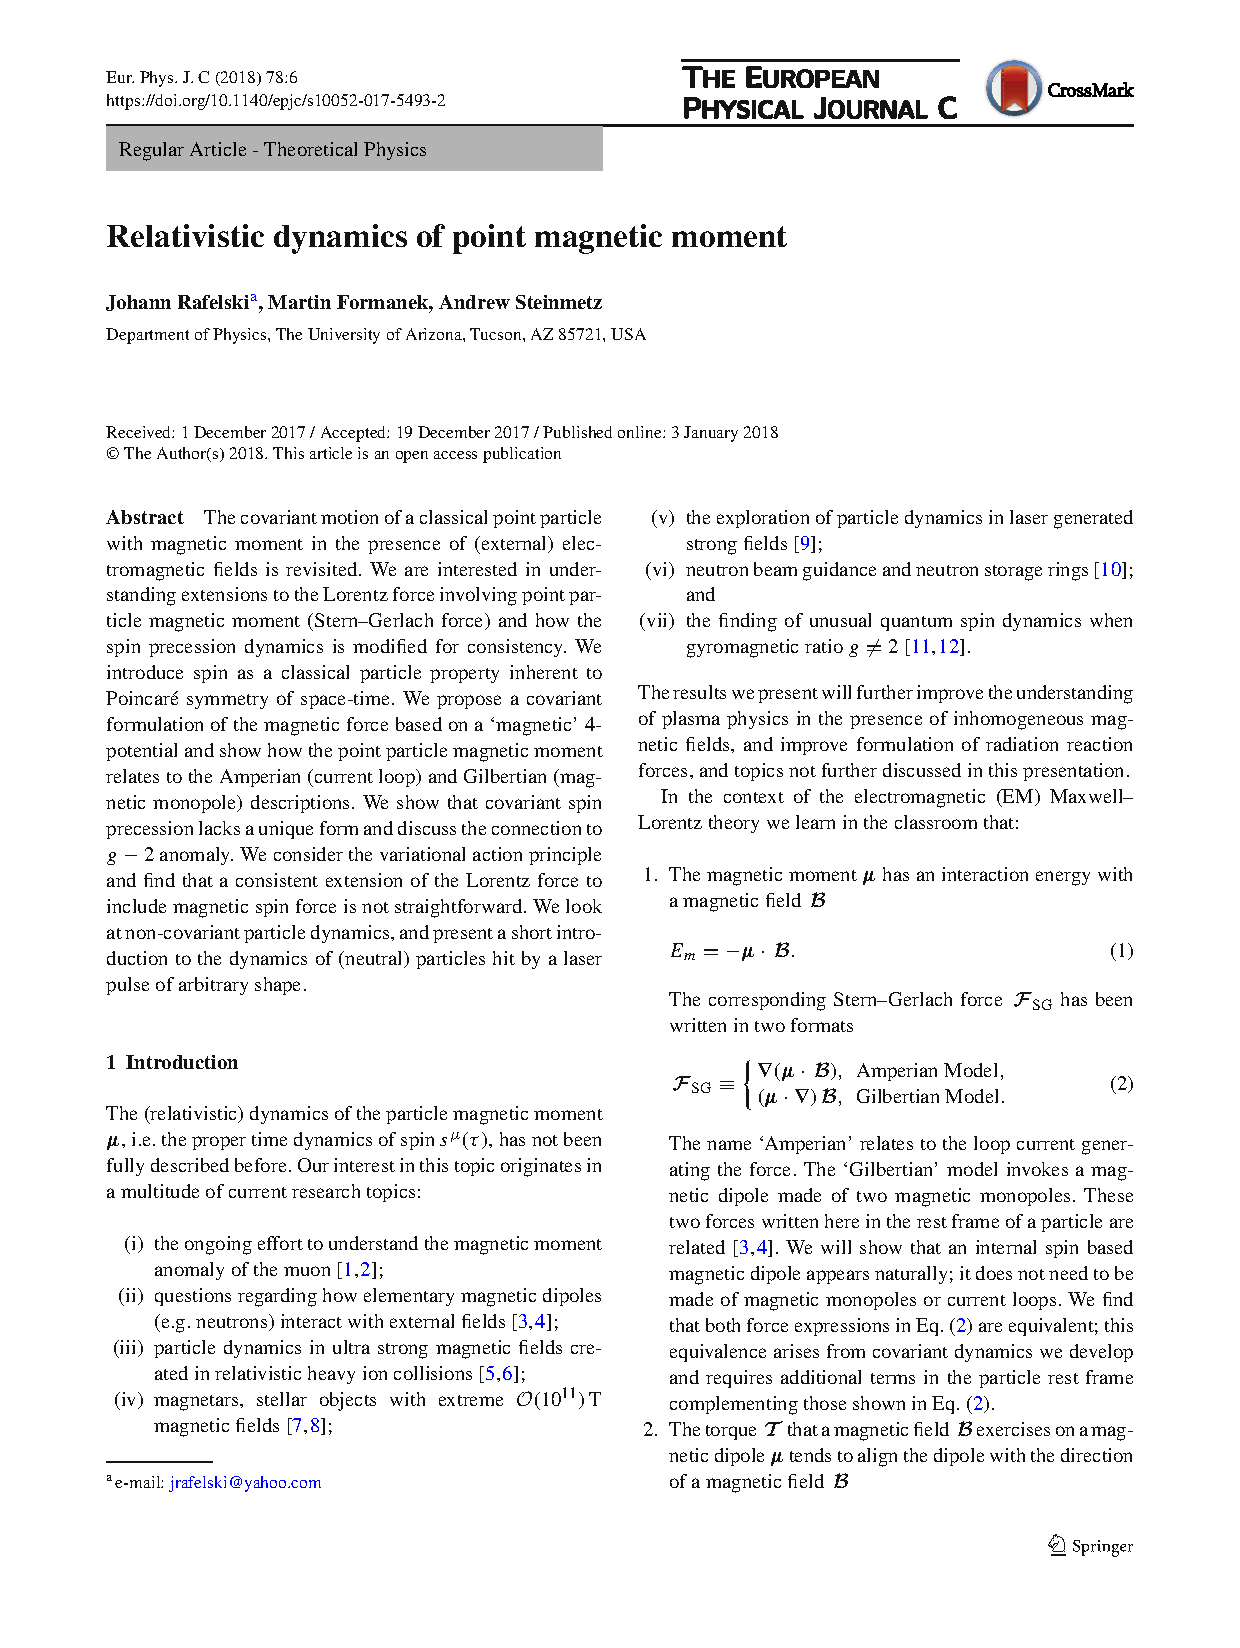
\includepdf[pages=-,pagecommand={},nup=1x2,landscape=true,width=5 in]{publications/rafelski2018relativistic.pdf}

%%%%%%%%%%%%%%%%%%%%%%%%%%%%%%%%%%%%%%%
%\chapter{Radiation reaction friction: Resistive material medium}
%%%%%%%%%%%%%%%%%%%%%%%%%%%%%%%%%%%%%%%
%\begin{center}
%Formanek, Martin, Andrew Steinmetz, and Johann Rafelski. "Radiation reaction friction: Resistive material medium." Physical Review D 102.5 (2020): 056015.

%doi: \href{10.1103/PhysRevD.102.056015}{10.1103/PhysRevD.102.056015}

%.

%Copyright (2020) by the American Physical Society

%This article is an open access article distributed under the terms and conditions of the Creative Commons Attribution %\href{https://creativecommons.org/licenses/by/4.0/}{(CC BY 4.0)} license.
%\end{center}
%\includepdf[pages=-,pagecommand={},nup=1x2,landscape=true,width=5 in]{publications/formanek2020relativistic.pdf}

%%%%%%%%%%%%%%%%%%%%%%%%%%%%%%%%%%%%%%%
\chapter{A Short Survey of Matter-Antimatter Evolution in the Primordial Universe}
\label{appendixD}
%%%%%%%%%%%%%%%%%%%%%%%%%%%%%%%%%%%%%%%
\begin{center}
Rafelski, J.; Birrell, J.; Steinmetz, A.; Yang, C.T. A Short Survey of Matter-Antimatter Evolution in the Primordial Universe. Universe 2023, 9, 309.
doi: \href{https://doi.org/10.3390/universe9070309}{10.3390/universe9070309}

.

Copyright (2023) by the authors. Licensee MDPI, Basel, Switzerland.

This article is an open access article distributed under the terms and conditions of the Creative Commons Attribution \href{https://creativecommons.org/licenses/by/4.0/}{(CC BY 4.0)} license.

\end{center}
\includepdf[pages=-,pagecommand={},nup=1x2,landscape=true,width=5 in]{publications/rafelski2023shortsurvey.pdf}


% Create the References list
\bibliographystyle{uabibnat}
\bibliography{bibs/chap01intro-refs,bibs/chap02moment-refs,bibs/chap03neutrino-refs,bibs/chap04cosmo-refs,bibs/chap06future-refs}

\end{document}
